% =============================================================================
%  Návod k softwaru HeatBattery
%  PDF zdroj odpovídající README_NAVOD.md.
%
%  Doporučený překladač:  xelatex  (kvůli UTF-8 / českým znakům)
%  Alternativa:           lualatex (totéž, jen jiný engine)
%
%  Sestavení (z této složky):
%      latexmk -xelatex navod.tex
%  nebo:
%      xelatex navod.tex && xelatex navod.tex
% =============================================================================

\documentclass[a4paper,11pt]{article}

% --- Stránka --------------------------------------------------------------
\usepackage[a4paper, margin=2.4cm, headheight=14pt]{geometry}
\usepackage{microtype}
\usepackage{parskip}

% --- Fonty a jazyk (xelatex / lualatex) -----------------------------------
\usepackage{fontspec}
\usepackage{polyglossia}
\setdefaultlanguage{czech}
% Vyber fontů – pokud nemáš nainstalované, smaž tyhle 3 řádky a TeX použije default.
\setmainfont{TeX Gyre Termes}
\setsansfont{TeX Gyre Heros}
\setmonofont{TeX Gyre Cursor}[Scale=0.92]

% --- Matematika -----------------------------------------------------------
\usepackage{amsmath, amssymb, mathtools}

% --- Tabulky --------------------------------------------------------------
\usepackage{booktabs}
\usepackage{longtable}
\usepackage{tabularx}
\usepackage{array}
\newcolumntype{L}[1]{>{\raggedright\arraybackslash}p{#1}}
\usepackage{needspace}

% --- Barvy a odkazy -------------------------------------------------------
\usepackage{xcolor}
\definecolor{cBg}{HTML}{F7F7F7}
\definecolor{cKw}{HTML}{0B5394}
\definecolor{cStr}{HTML}{B45F06}
\definecolor{cCmt}{HTML}{6A737D}
\definecolor{cFrame}{HTML}{D0D7DE}
\definecolor{cRule}{HTML}{1F77B4}

\usepackage[colorlinks=true,
            linkcolor=cRule,
            urlcolor=cRule,
            citecolor=cRule,
            bookmarksnumbered=true,
            pdftitle={Návod k softwaru HeatBattery},
            pdfauthor={HeatBattery}]{hyperref}
\usepackage{xurl}

% Odkaz na geometry.py z Example_01 (GitHub; větev master)
\newcommand{\GitHubExOneGeometryURL}{https://github.com/LiborKudela/heat-battery/blob/master/examples/Example_01/geometry.py}
\newcommand{\GitHubExOneGeometry}{\href{\GitHubExOneGeometryURL}{\texttt{geometry.py}}}
\newcommand{\GitHubExOneUnsteadyCSVURL}{https://github.com/LiborKudela/heat-battery/blob/master/examples/Example_01/results/unsteady.csv}
\newcommand{\GitHubExOneUnsteadyCSV}{\href{\GitHubExOneUnsteadyCSVURL}{\texttt{examples/Example\_01/results/unsteady.csv}}}
\newcommand{\GitHubExTwoDirURL}{https://github.com/LiborKudela/heat-battery/tree/master/examples/Example_02}
\newcommand{\GitHubExTwoDir}{\href{\GitHubExTwoDirURL}{\texttt{Example\_02}}}
\newcommand{\GitHubExFourDirURL}{https://github.com/LiborKudela/heat-battery/tree/master/examples/Example_04}
\newcommand{\GitHubExFourDir}{\href{\GitHubExFourDirURL}{\texttt{Example\_04}}}
\newcommand{\GitHubExFiveDirURL}{https://github.com/LiborKudela/heat-battery/tree/master/examples/Example_05}
\newcommand{\GitHubExFiveRunSize}{\href{\GitHubExFiveDirURL}{\texttt{examples/Example\_05/run\_example\_size5.py}}}
\newcommand{\GitHubProbingURL}{https://github.com/LiborKudela/heat-battery/blob/master/heat_battery/simulations/probing.py}
\newcommand{\GitHubProbing}{\href{\GitHubProbingURL}{\texttt{heat\_battery/simulations/probing.py}}}

% --- Seznamy a obsah ------------------------------------------------------
\usepackage{enumitem}
\setlist{itemsep=2pt, topsep=2pt}

% --- Code listings --------------------------------------------------------
\usepackage{listings}
\lstset{
  basicstyle=\ttfamily\small,
  keywordstyle=\color{cKw}\bfseries,
  stringstyle=\color{cStr},
  commentstyle=\color{cCmt}\itshape,
  backgroundcolor=\color{cBg},
  frame=single,
  rulecolor=\color{cFrame},
  framesep=4pt,
  xleftmargin=6pt,
  xrightmargin=6pt,
  breaklines=true,
  breakatwhitespace=false,
  breakindent=0pt,
  postbreak=\mbox{\textcolor{cCmt}{\ensuremath{\hookrightarrow}}\space},
  showstringspaces=false,
  columns=fullflexible,
  keepspaces=true,
  upquote=true,
  literate=%
    {á}{{\'a}}1 {č}{{\v c}}1 {ď}{{\v d}}1 {é}{{\'e}}1 {ě}{{\v e}}1
    {í}{{\'\i}}1 {ň}{{\v n}}1 {ó}{{\'o}}1 {ř}{{\v r}}1 {š}{{\v s}}1
    {ť}{{\v t}}1 {ú}{{\'u}}1 {ů}{{\r u}}1 {ý}{{\'y}}1 {ž}{{\v z}}1
    {Á}{{\'A}}1 {Č}{{\v C}}1 {Ď}{{\v D}}1 {É}{{\'E}}1 {Ě}{{\v E}}1
    {Í}{{\'I}}1 {Ň}{{\v N}}1 {Ó}{{\'O}}1 {Ř}{{\v R}}1 {Š}{{\v S}}1
    {Ť}{{\v T}}1 {Ú}{{\'U}}1 {Ů}{{\r U}}1 {Ý}{{\'Y}}1 {Ž}{{\v Z}}1
}

\lstdefinelanguage{Yaml}{
  morekeywords={true,false,null,~},
  morecomment=[l]{\#},
  morestring=[b]",
}

\lstdefinestyle{bash}{language=bash, keywords={mpirun,python,python3,bash,git,clone,cd,pip,sudo,apt,export,source}}
\lstdefinestyle{py}{language=Python}
\lstdefinestyle{yaml}{language=Yaml}
\lstdefinestyle{plain}{language=}

% Cele lstlisting bloky na jedné stránce (minipage se neláme mezi stránkami).
\usepackage{etoolbox}
\BeforeBeginEnvironment{lstlisting}{%
  \par\nointerlineskip
  \begin{minipage}[t]{\linewidth}%
}
\AfterEndEnvironment{lstlisting}{%
  \end{minipage}%
  \par
}

% --- Obrázky --------------------------------------------------------------
\usepackage{graphicx}
\usepackage{caption}
\usepackage{float}

% --- TikZ pro diagramy ----------------------------------------------------
\usepackage{tikz}
\usetikzlibrary{positioning, arrows.meta, fit, backgrounds, shapes.geometric}

% --- Vizuální placeholder pro chybějící obrázky ---------------------------
% Použití:  \figplaceholder[výška]{popis, který se objeví uvnitř rámečku}
\newcommand{\figplaceholder}[2][6cm]{%
  \begin{center}
  \fbox{%
    \begin{minipage}[c][#1][c]{0.92\linewidth}
      \centering
      \footnotesize\itshape\color{cCmt}
      [\,placeholder pro obrázek\,]\par\medskip
      #2
    \end{minipage}%
  }
  \end{center}
}

% --- Boxy pro poznámky / citace -------------------------------------------
\usepackage[most]{tcolorbox}
\newtcolorbox{noteblock}[1][]{%
  colback=cBg, colframe=cRule!60!black, boxrule=0.4pt,
  left=8pt, right=8pt, top=4pt, bottom=4pt, arc=2pt,
  enhanced, breakable, #1
}

% --- Drobnosti ------------------------------------------------------------
\renewcommand{\arraystretch}{1.15}

\title{\textbf{Návod k softwaru HeatBattery}\\[0.3em]
       \large simulace tepelných akumulátorů}
\author{Tým HeatBattery}
\date{\today}

% =============================================================================
\begin{document}
\maketitle

\noindent
Tento dokument je český průvodce balíčkem softwaru \textbf{HiTepOptim} \ (\texttt{heat\_battery}). Stručný
anglický přehled najdete v kořenovém souboru
\href{../../README.md}{\texttt{README.md}}; tento návod jde více do hloubky
a popisuje, jak se kód v repozitáři skládá a jak se používá v praxi.

\begin{noteblock}
\textbf{Průběžná dokumentace v kódu.}
Většina tříd, metod a funkcí v softwaru má vlastní docstring. Moderní IDE
(například VS Code / Cursor, PyCharm nebo Spyder) tyto docstringy načítá přímo při psaní kódu,
zobrazuje je v našeptávání a dovoluje rychle přejít na definici daného objektu.
Pro konkrétní argumenty funkcí, návratové hodnoty a aktuální chování API je to
často nejpřesnější zdroj dokumentace v daném okamžiku.
\end{noteblock}

\begin{center}
\makebox[\linewidth][c]{%
  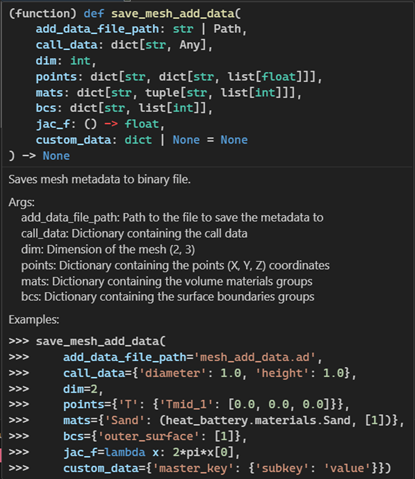
\includegraphics[width=0.46\linewidth]{images/vscode-docstring.png}%
}
\par\smallskip
\small\emph{Docstring jako kontextová nápověda přímo při práci s kódem.}
\end{center}

\hrulefill

\tableofcontents

\hrulefill

% =============================================================================
\section{Účel a architektura}\label{sec:ucel}

\subsection*{Představení softwaru}

Nástroj \textbf{HiTepOptim} (v repozitáři jako balíček
\texttt{heat\_battery}) je soubor navazujících softwarových komponent pro
definici, simulaci, systematické studie a vizualizaci výsledků systémů
využívajících vysokoteplotní akumulaci tepla ve formě \textbf{citelného tepla}.
Jeho základem je přednastavený MKP řešič vedení tepla, který umožňuje sledovat
detailní prostorové rozložení teploty v akumulátoru.

Akumulátor obvykle nevystupuje jako izolovaný objekt, ale jako část většího
energetického systému. S okolním modelem, často popsaným jednodušším 1D
přístupem, si vyměňuje energii přes okrajové podmínky (například předávání
tepla povrchem) nebo přes objemové zdrojové členy (například elektrický odporový
ohřev topnými patronami). Geometrie akumulátoru proto ovlivňuje nejen celkovou
kapacitu, ale i dynamiku maximálního nabíjecího a vybíjecího výkonu. Nevhodné
uspořádání může omezit výkon i tehdy, když je akumulátor z hlediska celkové
energie nabitý, nebo může vést k lokálnímu přehřívání topidel.

Simulace několikaletého provozu vytvářejí velké objemy dat, zejména časové řady
sond s jemným časovým krokem. U parametrických studií tento objem dále roste.
Součástí nástroje je proto i databázové zázemí a webové rozhraní pro
interaktivní prohlížení výsledků v grafech. Cílem není skrýt fyzikální podstatu
modelu, ale omezit množství rutinních kroků spojených se sestavením, stabilizací
a vyhodnocením MKP výpočtu.

Software obsahuje několik příkladů, které slouží k ověření instalace i jako
vzor pro vlastní úpravy. Současná verze pracuje s omezeným výběrem materiálů a
komponent navazujícího systému (například FVE, budova nebo PID řízení), ale
způsob zadávání zůstává flexibilní díky Pythonu a připravenému vysokoúrovňovému
rozhraní. Do budoucna se počítá s rozšířením komponent i vlastností
teplonosných médií, například vzduchu a vody.

Hlavním účelem softwaru je poskytnout cestu k odbornému zhodnocení systémů
akumulace energie ve formě citelného tepla v různých aplikačních kontextech
(domácnosti, sídliště, průmysl nebo energetika). Nástroj je určený pro uživatele,
kteří jsou schopni správně definovat fyzikální systém, ale nemají se při každé
studii zabývat všemi technickými detaily MKP implementace. Není zamýšlen jako
aplikace pro širokou veřejnost. Je sestaven výhradně z open-source komponent a
instalační skript je připraven pro Ubuntu, včetně použití přes WSL na počítačích
s Windows.

\subsection*{Modelový přístup}

Model popisuje chování tepelného akumulátoru jako součásti širšího energetického
systému. Uživatel zadává zejména geometrii akumulátoru, materiály, zdroje tepla,
okrajové podmínky a vazby na zbytek systému. Software se skládá z několika
částí:

\begin{itemize}
  \item simulačního jádra pro ko-simulaci akumulátoru (MKP) se zbytkem systému
        a pro numericky stabilní řízení časového výpočtu,
  \item sestavení MKP úlohy akumulátoru a jejích objemových i okrajových členů
        podle zadané geometrie,
  \item databázové vrstvy pro ukládání výsledků jednotlivých simulací a
        parametrických studií,
  \item webového rozhraní pro práci s databází, především pro vizualizaci
        výsledků.
\end{itemize}

\subsection*{Model akumulátoru}

Výpočtový model akumulátoru je implementován jako Python knihovna. Jeho hlavním
vstupem je geometrie, která může vznikat parametricky z Python funkce a následně
se předává simulační třídě. Geometrická metadata obvykle obsahují:

\begin{itemize}
  \item síť ve formátu Gmsh \texttt{.msh} s fyzikálními skupinami pro objemy a
        části hranice,
  \item argumenty funkce, která geometrii vygenerovala,
  \item dimenzionalitu úlohy, zpravidla 2D nebo 3D,
  \item body pro sondy, například pro záznam teplot,
  \item přiřazení materiálů k objemovým podoblastem,
  \item pojmenované části hranice pro okrajové podmínky,
  \item Jakobián pro symetrie nebo jinou úpravu integrační míry,
  \item další údaje vzniklé při generování geometrie, například délky nebo počty
        kanálů.
\end{itemize}

Schéma níže ukazuje zjednodušený tok dat od vstupů přes výpočetní jádro až
k výstupům.

\begin{center}
\begin{tikzpicture}[
    box/.style    = {draw, rounded corners=2pt, align=center,
                     minimum height=0.85cm, minimum width=3.4cm,
                     inner sep=4pt, font=\small, fill=cBg},
    arr/.style    = {-{Stealth[length=2.2mm]}, thick, color=cRule},
    darr/.style   = {-{Stealth[length=2.2mm]}, dashed, color=cRule!70}
]
% --- Sloupce: x souradnice -----------------------------------------------
\def\xIn{0}
\def\xCore{5.0}
\def\xOut{10.0}

% --- Vstupy (vlevo) ------------------------------------------------------
\node[box] (gmsh)  at (\xIn, 2.6)  {Gmsh síť \texttt{.msh + .ad}};
\node[box] (mat)   at (\xIn, 1.4)  {Materiály};
\node[box] (meteo) at (\xIn, 0.2)  {PVGIS / měření};

% --- Jadro (uprostred) -- bezi v MPI prostredi ---------------------------
\node[box] (sim)   at (\xCore, 1.4)  {\texttt{Simulation} + Termy};
\node[box] (sol)   at (\xCore, 0.2)  {SNES (Newton) + KSP};

% MPI prostredi - obal jadra (Sim + Sol); inner sep = vzduch uvnitr ohraniceni
\node[draw=cRule!70!black, dashed, rounded corners=5pt, line width=0.55pt,
      inner sep=16pt, inner xsep=18pt,
      fit=(sim)(sol),
      label={[font=\scriptsize\bfseries, color=cRule!70!black,
              anchor=south west, xshift=10pt, yshift=2pt]north west:%
             MPI prostředí (\texttt{mpirun -n N})}] (mpi) {};

% --- Vystupy (vpravo): XDMF nahore, Checkpointy uprostred, Sondy dole ------
% (o jeden radek nize nez prvni dva sloupce: krok 1.2)
\node[box] (xd)    at (\xOut, 1.4)  {XDMF \texttt{.xdmf + .h5}};
\node[box] (cp)    at (\xOut, 0.2)  {Checkpointy};
\node[box] (pr)    at (\xOut,-1.0)  {Sondy: paměť / CSV / DB};

% --- Orchestrace (dole, vystredeno pod MPI) -----------------------------
\node[box] (pg)    at (\xCore, -2.4)  {PostgreSQL Project};
% Webove rozhrani (nad daty z projektu) -----------------------------------
\node[box, align=center, minimum width=3.6cm] (web) at (\xOut, -2.4)
  {Webové rozhraní\\[-0.12em]{\scriptsize vizualizace (Dash / Plotly)}};

% --- Hrany: vstupy -> jadro (proniknou do MPI ramecku, rozprostrene cile) ---
\draw[arr] (gmsh.east)  -- ([yshift= 2.8mm]sim.west);
\draw[arr] (mat.east)   -- (sim.west);
\draw[arr] (meteo.east) -- ([yshift=-2.8mm]sim.west);

% Sim <-> SNES (uvnitr MPI prostredi)
\draw[arr] (sim.south)  -- (sol.north);

% --- Hrany: jadro -> vystupy (vsechny tri sikmo z SNES) -------------------
\coordinate (soli) at ([yshift= 2.8mm]sol.east);
\coordinate (solm) at (sol.east);
\coordinate (sols) at ([yshift=-2.8mm]sol.east);
\draw[arr] (soli) -- ([yshift= 2.0mm]xd.west);
\draw[arr] (solm) -- (cp.west);
\draw[arr] (sols) -- ([yshift=-2.0mm]pr.west);

% --- Orchestrace: smycka MPI <-> PostgreSQL -----------------------------
% parametrizace (dolu, dashed): MPI -> PG, posunuto vlevo
\draw[darr] ([xshift=-1.0cm]mpi.south)
  -- node[left, font=\scriptsize] {parametrizace}
     ([xshift=-1.0cm]pg.north);
% uloha (nahoru, solid): PG -> MPI, posunuto vpravo
\draw[arr]  ([xshift= 1.0cm]pg.north)
  -- node[right, font=\scriptsize] {úloha}
     ([xshift= 1.0cm]mpi.south);
% PostgreSQL -> webove rozhrani (prehled vysledku z DB)
\draw[arr] (pg.east) -- node[above, font=\scriptsize, align=center]
  {sondy /\\ stav úloh} (web.west);
\end{tikzpicture}
\end{center}

\noindent\textbf{Cílová skupina:} výzkumní pracovníci a studenti, kteří mají
základní zkušenost s Pythonem a prostředím \textbf{Linux} (doporučené jsou
Ubuntu 22.04 nebo 24.04). U distribuovaných studií se navíc předpokládá
\textbf{PostgreSQL}, dostupné \textbf{MPI} v clusteru a síťový přístup
k databázi z výpočetních uzlů.

% =============================================================================
\section{Požadavky a instalace}\label{sec:install}

\subsection*{Systém a závislosti}

\begin{itemize}
  \item \textbf{Operační systém:} Linux. Ve Windows použijte
        \textbf{WSL} s distribucí Ubuntu; další kroky jsou stejné jako
        v nativním Linuxu (viz odkazy v \texttt{README.md}).
  \item \textbf{Software:} Python 3.8 nebo novější, \textbf{DOLFINx / FEniCSx},
        \textbf{PETSc}, \textbf{MPI}; pro generování sítě typicky \textbf{Gmsh}.
        Kompletní závislosti jsou uvedeny v \texttt{pyproject.toml}.
  \item \textbf{Volitelně:} \textbf{ParaView} pro prostorovou vizualizaci výstupů
        ve formátu XDMF.
\end{itemize}

\subsection*{Postup instalace}

\begin{lstlisting}[style=bash]
git clone https://github.com/LiborKudela/heat-battery.git
cd heat-battery
bash install_scripts/install_ubuntu.sh --help
\end{lstlisting}

Nejčastější varianty:

\Needspace{14\baselineskip}%
\begin{minipage}{\linewidth}
{\small\emph{Výpočetní worker bez lokální databáze:}}%
\nopagebreak

\begin{lstlisting}[style=bash]
bash install_scripts/install_ubuntu.sh -y
\end{lstlisting}
\end{minipage}

\medskip
\Needspace{16\baselineskip}%
\begin{minipage}{\linewidth}
{\small\emph{Worker včetně PostgreSQL (v clusteru stačí jeden tento uzel):}}%
\nopagebreak

\begin{lstlisting}[style=bash]
bash install_scripts/install_ubuntu.sh -y -p --ppass HESLO --ppassc HESLO
\end{lstlisting}
\end{minipage}

Heslo si zvolte a zapište je do lokálního souboru \texttt{config.yaml}
(podrobnosti v~\autoref{sec:config}). Tento soubor pak umístěte do pravocní
složky jednotlivých pracovních uzlů clusteru (databázový uzel může být zároveň
pracovním uzlem, ale nikoliv naopak). Pokud chcete nainstalovat software na OS 
Windows (10/11)  - je jediným prověřeným způsobem cesta přes Windows Subsystem
for Linux (WSL). Ideální je nainstalovat distribuci Ubuntu ve které pak proběhne
instalace stejně jako na standardním Ubuntu systému.

\subsection*{Ověření instalace}

\begin{lstlisting}[style=bash]
python3 -c "import heat_battery; heat_battery.test_package()"
\end{lstlisting}

Tento příkaz otestuje několik předefinovaných testů a
odsimuluje velmi krátké simulace. Následně reportuje úspěšné dokončení nebo 
selhání těchto testů.

% =============================================================================
\section{Rychlý start}\label{sec:start}

Následují tři běžné způsoby práce podle toho, co chcete spustit.

\subsection*{A. Rychlá lokální simulace (jeden případ bez databáze)}

Nejjednodušší varianta spouští \texttt{solve\_unsteady} přímo, ukládá sondy
do lokálních CSV souborů a případně zapisuje XDMF. Fronta úloh v PostgreSQL se
v tomto režimu nepoužívá. Můžeme tak spustit například přiloženou ukázku:

\begin{lstlisting}[style=bash]
mpirun -n 4 python3 -m examples.Example_05.run_example_size5
\end{lstlisting}

Skript \GitHubExFiveRunSize{} ukazuje načtení
geometrie (s mezipamětí přes \texttt{CachedGeometryBuilder}), nastavení
checkpointů do lokálního adresáře a spuštění jednoho samostatného výpočtu.

\subsection*{B. Rozsáhlá parametrická studie na clusteru (PostgreSQL a worker procesy)}

Parametrická studie, fronta úloh a výpočetní workery vyžadují platný lokální
soubor \texttt{config.yaml}. Obvykle stačí doplnit údaje pro připojení
k PostgreSQL; ostatní parametry mají použitelné výchozí hodnoty v souboru
\texttt{heat\_battery/base\_config.yaml}. Podrobnosti jsou v~\autoref{sec:config},
zejména v~\hyperref[sec:config-minimal]{bloku o minimálním nastavení}.

\begin{enumerate}
  \item \textbf{Naplnit frontu úloh v databázi} (na jednom z worker uzlů)
\begin{lstlisting}[style=bash]
python3 -m examples.Example_05.run_example
\end{lstlisting}
  \item \textbf{Spustit pracovní smyčku na jednom nebo více uzlech}
\begin{lstlisting}[style=bash]
mpirun -n 4 python3 worker.py --num-jobs 5 --project project_example_05
\end{lstlisting}
\begin{noteblock}
\textbf{Poznámka k příkazu.}
\texttt{-n 4} spustí čtyři MPI procesy. Hodnotu \texttt{-n} volte podle
počtu fyzických CPU jader dostupných na daném uzlu. Pro běh jedné simulace přes
více uzlů je potřeba nastavit MPI spouštění přes seznam hostů (např.\
\href{https://docs.open-mpi.org/en/v5.0.6/launching-apps/scheduling.html}{Open MPI hostfile})
a zajistit sdílené úložiště dostupné ze všech uzlů (např.\
\href{https://documentation.ubuntu.com/server/how-to/networking/install-nfs/index.html}{NFS na Ubuntu Serveru}).
Je však potřeba zohlednit overhead způsobený síťovou komunikací mezi uzly (někdy může být méně více).
\end{noteblock}
  \item \textbf{Sledovat průběh přes webový dashboard}
\begin{lstlisting}[style=bash]
python3 examples/Example_05/view_project.py
\end{lstlisting}
\end{enumerate}



% =============================================================================
\section{Konfigurace (\texttt{config.yaml})}\label{sec:config}

Modul \texttt{heat\_battery/config.py} skládá konfiguraci ze dvou zdrojů:

\begin{enumerate}
  \item \textbf{Globální šablonu} ze souboru \texttt{heat\_battery/base\_config.yaml}.
  \item \textbf{Lokální doplněk} \texttt{config.yaml} z aktuálního pracovního
        adresáře, pokud soubor existuje (konstanta \path{LOCAL_CONFIG_FILE_PATH}).
\end{enumerate}

Hodnoty z lokálního souboru \textbf{přepisují} globální šablonu. Pokud lokální
soubor obsahuje klíč, který v šabloně neexistuje, slučování konfigurace skončí
chybou (\texttt{merge\_configs}). Je to záměrná kontrola proti překlepům. Pro
nestandardní umístění konfiguračních souborů slouží
\texttt{setup\_global\_config\_path} a \texttt{setup\_local\_config\_path}.

\phantomsection\label{sec:config-minimal}
\begin{noteblock}
\textbf{Minimální lokální konfigurace bez databáze}

Globální šablona \texttt{heat\_battery/base\_config.yaml} už obsahuje většinu
nastavení a jedná se funční tovární výchoxí nastavení. Výpočty nevyžadující 
PostgreSQL databázi si s tímto továrním nastavením bohatě vystačí (např.\ \texttt{run\_example\_size5} a většina
\texttt{examples/Example\_01--04}).

\textbf{Minimální lokální konfigurace s PostgreSQL databází}

Tovární nastavení je nutné rozšířit minimálně o přístupové údaje do PostgreSQL
databáze a doporučuje se nastavit i uživatelské jméno pro snadnější určení
vlastnictví zadání simulací v databázi. Níže jsou uvedenty parametry,
kterých se tyto změny týkají.
\end{noteblock}

\phantomsection\label{sec:config-important}
\subsection*{Důležité položky \texttt{base\_config.yaml}}

\begin{itemize}
  \item \texttt{user} (kořen konfigurace, nikoli \texttt{database.postgres.user}) ---
        metadata o autorovi. I při hodnotách \texttt{null} lze úlohy do fronty
        zařazovat; údaj se ukládá ve sloupci \texttt{created\_by}. Pro přehled
        a dohledatelnost autora ve webovém rozhraní jej doporučujeme vyplnit,
        (zejména pokud do jednoho projektu vkládá zadaní více uživatelů).
        Údaje není potřeaba vyplnit všechny.
  \item \texttt{local\_temp\_dir} (výchozí \texttt{heat\_battery\_temp}, který 
        se umístí do cwd worker procesu) ---
        adresář, do kterého worker na výpočetním uzlu rozbalí zdrojové soubory
        úlohy stažené z databáze. Na daném uzlu musí být zapisovatelný a musí
        mít dostatek volného místa.
  \item \texttt{database.use\_engine} --- musí zůstat \texttt{postgresql};
        jiné databázové rozhraní není v tomto repozitáři implementováno.
  \item \phantomsection\label{sec:config-postgres}%
        \texttt{database.postgres} --- parametry připojení knihovny \texttt{psycopg2}.

        \begin{itemize}
          \item \texttt{db\_name} --- název databáze PostgreSQL, v níž aplikace
                ukládá svá data (např.\ \path{heat_battery}).
          \item \texttt{user} --- obvykle \texttt{postgres}, pokud instalaci provedl
                dodávaný instalační skript; jinak účet přidělený správcem databázového
                serveru.
          \item \texttt{password} --- heslo zvolené při instalaci skriptem nebo heslo
                od správce serveru.
          \item \texttt{host} --- typicky veřejná IP adresa počítače, na němž je
                PostgreSQL nainstalován a zpřístupněn; při běhu na témže stroji
                často \texttt{localhost}.
          \item \texttt{port} --- číslo TCP portu (celé číslo); standardní instalace
                používá \texttt{5432}. Při nestandardním čísle portu uveďte např.\
                \texttt{5433}.
        \end{itemize}

\end{itemize}

\subsection*{Úplný obsah \texttt{heat\_battery/base\_config.yaml}}

Níže je kompletní obsah globální šablony z repozitáře. Lokální
\texttt{config.yaml} k ní přidává pouze přepsání vybraných klíčů.

\begin{minipage}[t]{\linewidth}
\lstinputlisting[style=yaml]{../../heat_battery/base_config.yaml}
\end{minipage}

% =============================================================================
\section{Matematický model a slabá formulace}\label{sec:math}

Model řeší \textbf{MKP úlohu vedení tepla} na neuspořádané síti: geometrie
a fyzikální skupiny vznikají v Gmsh, vlastní výpočet běží v DOLFINx. Časová
diskretizace používá \textbf{$\theta$-schéma}; při výchozí hodnotě
\texttt{theta = 0.5} odpovídá metodě \textbf{Crank--Nicolson}. Nelineární část
každého časového kroku řeší \textbf{SNES} z PETSc, lineární podsystémy pak
\textbf{KSP}.

\subsection*{Slabá formulace (v souladu s implementací)}

Nechť \(T\) je teplotní pole na nové časové hladině, \(T_n\) pole z předchozího
kroku, \(v\) libovolná testovací funkce a \(J\) Jakobián souřadnic
(v kódu \texttt{self.jac}). Sumy probíhají přes materiálové podoblasti
\(\Omega_j\) a pojmenované části hranice \(\Gamma\). Pro \(\theta = 0.5\) platí:

\begin{equation*}
\begin{aligned}
\mathcal{R}(T;v)\;=\;
&\sum_{j}\!\int_{\Omega_j}\!\Bigl[\rho(T)\,c_p(T)\,T-\rho(T_n)\,c_p(T_n)\,T_n\Bigr]\,v\,J\,\mathrm{d}x\\
&+\theta\,\Delta t\sum_{j}\!\int_{\Omega_j}\!\Bigl[k(T)\,\nabla T\!\cdot\!\nabla v - q_{\mathrm{vol}}(T,\mathbf{x},t)\,v\Bigr]\,J\,\mathrm{d}x\\
&+(1-\theta)\,\Delta t\sum_{j}\!\int_{\Omega_j}\!\Bigl[k(T_n)\,\nabla T_n\!\cdot\!\nabla v - q_{\mathrm{vol}}(T_n,\mathbf{x},t_n)\,v\Bigr]\,J\,\mathrm{d}x\\
&+\theta\,\Delta t\sum_{\Gamma}\!\int_{\Gamma} g_{\mathrm{bc}}(T,\mathbf{x},t)\,v\,J\,\mathrm{d}s\\
&+(1-\theta)\,\Delta t\sum_{\Gamma}\!\int_{\Gamma} g_{\mathrm{bc}}(T_n,\mathbf{x},t_n)\,v\,J\,\mathrm{d}s\;=\;0\quad\forall v.
\end{aligned}
\end{equation*}

Slovně: reziduum kombinuje časovou změnu tepelného stavu, přibližně daného
entalpií \(\rho c_p T\), s \(\theta\)-váženým příspěvkem nelineární
\textbf{difuze} \(k(T)\nabla T\), \textbf{objemových zdrojů}
\(q_{\mathrm{vol}}\) a \textbf{okrajových toků} \(g_{\mathrm{bc}}\). Objemové
zdroje přicházejí přes termy \texttt{q\_source} a ve slabé formulaci vystupují
se znaménkem~\(-\); okrajové členy přicházejí přes \texttt{bcs\_terms}
se znaménkem~\(+\).

\begin{noteblock}
\textbf{Poznámka.}
V budoucí verzi bude v časovém členu slabé formulace použita přímo
\textbf{entalpie} místo současného modelování skrze výraz \(\rho\,c_p\,T\).
\end{noteblock}

Nastavení tolerancí, časové integrace, výstupů a doplňkových voleb numerického
řešiče (včetně režimu \texttt{solve\_steady}) je popsáno v~\autoref{sec:sim}.

% =============================================================================
\section{Práce se simulací (\texttt{Simulation})}\label{sec:sim}

\texttt{Simulation} je základní třída pro vlastní model akumulátoru. V běžném
použití ji uživatel neinstancuje přímo, ale vytvoří z ní odvozenou třídu, která
popíše konkrétní fyziku dané úlohy: zdroje tepla, okrajové podmínky, sondy a
uživatelsky pohodlné rozhraní pro spuštění výpočtu. Příklady v repozitáři tuto
strukturu používají důsledně; typicky stačí převzít jeden z nich a upravit
geometrii, materiály a několik metod modelové třídy.

Z praktického pohledu jsou při práci se simulací důležité čtyři kroky:

\begin{enumerate}
  \item \textbf{Připravit geometrii a metadata} -- adresář \texttt{geometry\_dir}
        musí obsahovat síť \texttt{.msh} a odpovídající \texttt{.ad} soubor.
        Název modelu v \texttt{model\_name} musí odpovídat názvu těchto souborů
        bez přípony.
  \item \textbf{Odvodit modelovou třídu ze \texttt{Simulation}} -- v ní se
        napojí termy na pojmenované objemy a části hranice a nadefinují se sondy.
  \item \textbf{Rozhodnout, co se má počítat} -- pro rovnovážný stav slouží
        \texttt{solve\_steady}, pro časový průběh \texttt{solve\_unsteady}.
  \item \textbf{Nastavit výstupy} -- podle potřeby se zapínají CSV/DB sondy,
        XDMF pole pro ParaView a checkpointy pro pokračování přerušeného běhu.
\end{enumerate}

\begin{center}
\begin{tikzpicture}[
    stepbox/.style={draw, rounded corners=2pt, align=center, fill=cBg,
                    minimum width=3.0cm, minimum height=0.95cm,
                    inner sep=4pt, font=\small},
    arr/.style={-{Stealth[length=2.2mm]}, thick, color=cRule},
    node distance=0.78cm and 0.9cm
]
\node[stepbox] (geo) {Geometrie\\\texttt{.msh + .ad}};
\node[stepbox, right=of geo] (load) {\texttt{load\_geometry}\\tagy, materiály};
\node[stepbox, right=of load] (terms) {Termy a sondy\\v odvozené třídě};
\node[stepbox, below=of terms] (solve) {\texttt{solve\_steady}\\nebo \texttt{solve\_unsteady}};
\node[stepbox, left=of solve] (solver) {SNES / KSP\\časový krok};
\node[stepbox, left=of solver] (out) {Výstupy\\sondy, XDMF, checkpoint};

\draw[arr] (geo) -- (load);
\draw[arr] (load) -- (terms);
\draw[arr] (terms) -- (solve);
\draw[arr] (solve) -- (solver);
\draw[arr] (solver) -- (out);
\end{tikzpicture}
\par\smallskip
\small\emph{Zjednodušený životní cyklus modelu od geometrie po výstupy.}
\end{center}

\subsection*{Životní cyklus konstruktoru}

Při vytvoření objektu modelu proběhne většina technické přípravy automaticky.
Uživatel obvykle potřebuje vědět hlavně to, že názvy použité v kódu musí sedět
na názvy fyzikálních skupin uložené v geometrii. Po zadání \texttt{geometry\_dir}
a \texttt{model\_name} konstruktor:

\begin{enumerate}
  \item \texttt{load\_geometry} načte \texttt{.msh} a \texttt{.ad} metadata
        a vytvoří \texttt{domain}, \texttt{cell\_tags}, \texttt{facet\_tags},
        materiálové objekty a mapy názvů podoblastí.
  \item Vytvoří integrační míry (\texttt{dx}, \texttt{ds}, \texttt{dS}),
        funkční prostory a teplotní pole potřebná pro MKP výpočet.
  \item Spočítá objemy materiálových podoblastí a plochy hraničních částí.
        Tyto hodnoty se používají například při normalizaci zdrojů a sond.
  \item Zavolá \texttt{define\_form\_subdomain\_terms}, kde odvozený model
        připojí zdroje a okrajové podmínky přes \texttt{set\_source\_term} a
        \texttt{set\_bc\_term}.
  \item Podle nastavení argumentu \texttt{build\_solvers} sestaví potřebné řešiče. Pokud víte, že
        budete spouštět pouze časový výpočet, není nutné sestavovat všechny
        varianty.
\end{enumerate}

\subsection*{Co se typicky přepisuje}

V jednoduchém modelu obvykle stačí přepsat dvě až čtyři metody:

\begin{itemize}
  \item \texttt{define\_form\_subdomain\_terms} -- přiřadí zdroje a okrajové
        podmínky k pojmenovaným částem geometrie.
  \item \texttt{create\_common\_probes} -- zaregistruje veličiny, které chcete
        sledovat v čase, například teploty v bodech nebo celkovou energii.
  \item \texttt{solve\_steady} -- volitelný obal pro stacionární výpočet. Hodí
        se, pokud chcete uživateli nabídnout několik pojmenovaných parametrů
        místo ručního nastavování konstant v termech.
  \item \texttt{solve\_unsteady} -- obdobný obal pro časový výpočet. Typicky
        převádí funkce času z run-skriptu na aktualizační callbacky termů.
\end{itemize}

Podrobnější ukázka těchto přepisů je v tutoriálu Example\_01 v následující
kapitole. Při tvorbě nového modelu je praktické nejprve zprovoznit minimální
stacionární nebo krátký nestacionární výpočet, teprve potom přidávat checkpointy,
XDMF výstupy a delší časové horizonty.

\subsection*{Volby numerického řešiče}

Slabá formulace se při běhu sestaví a předá nelineárnímu řešiči SNES a
lineárnímu řešiči KSP z PETSc. V praxi se k numerickým volbám sahá hlavně ve
chvíli, kdy výpočet konverguje pomalu, časový krok se příliš zmenšuje nebo se
model chová výrazně nelineárně. Úplný seznam provozních parametrů, včetně
časových kroků a výstupů, je v docstringách metod a v tabulce
v~\hyperref[pars:solve-unsteady]{následující podsekci}.

\subsubsection*{Tolerance SNES a KSP}
Parametry \texttt{atol}, \texttt{rtol}, \texttt{stol} a volitelně
\texttt{ksp\_rtol} určují kritéria ukončení iterací SNES a přidruženého KSP.
Používají se u stacionárního i nestacionárního řešení. Při prvních pokusech je
vhodné začít s výchozími hodnotami a měnit je až ve chvíli, kdy solver opakovaně
selhává nebo je zbytečně pomalý.

\subsubsection*{Vnější iterace nad Termy}
Některé objekty \texttt{Term} mohou při ko-simulaci potřebovat uvnitř jednoho
časového kroku dodatečné vnější iterace. Parametr \texttt{max\_term\_its}
nastavuje jejich horní mez. Přepínač \texttt{force\_explicit\_terms} tuto smyčku
vypne; příslušné termy se pak vyhodnotí pouze jednou na začátku kroku. Takový
režim je vhodný jen tam, kde to dává fyzikální smysl a kde nevadí explicitní
vazba mezi akumulátorem a okolním systémem (to je tam kde termy ovlivňují 
akumulátor, ale akumulátor neovlivňuje termy).

\subsubsection*{Projekce teploty v čase}
Volba \texttt{use\_time\_projection} zapíná lineární extrapolaci pole \(T\) z
předchozích časových hladin jako počáteční odhad pro Newtonovu metodu; typicky
snižuje počet nelineárních iterací. U prudkých změn řízení nebo okrajových
podmínek je ale vhodné sledovat, zda projekce nezhoršuje počáteční odhad.

\begin{noteblock}
\textbf{Poznámka k dalšímu vývoji.}
Budoucí verze bude mít pokročilejší systém explicitního odhadu řešení pro nový
časový krok, například extrapolaci vyššího řádu (kubickou apod.).
\end{noteblock}

\subsubsection*{Stacionární režim}
Metoda \texttt{solve\_steady} řeší stejnou rodinu Termů bez časové diskretizace
a slouží k výpočtu rovnovážného teplotního pole. Prakticky se hodí pro kontrolu
geometrie, materiálů a znamének okrajových podmínek před spuštěním dlouhé
časové simulace.

\subsection*{\texttt{solve\_unsteady} -- parametry pro běžné použití}
\phantomsection\label{pars:solve-unsteady}

Čas je v sekundách \textbf{simulovaného modelu} (ne reálného běhu). Pro první
ověření modelu volte krátký \texttt{t\_max}, častější výpis sond a raději
menší \texttt{dt\_max}; pro produkční běh pak nastavte výstupy tak, aby objem
dat odpovídal tomu, co opravdu potřebujete vyhodnocovat.

\begin{longtable}{@{}L{5.6cm} L{9.5cm}@{}}
\toprule
\textbf{Parametr} & \textbf{Význam} \\
\midrule
\endhead
\texttt{T0}, \texttt{T\_guess}, \texttt{h0\_T\_ref}
  & Počáteční teplota / Newtonův odhad / referenční teplota pro entalpii. \\
\texttt{t\_max}
  & Konec simulace v simulovaném čase. \\
\texttt{dt\_start}, \texttt{dt\_min}, \texttt{dt\_max}
  & Počáteční krok a jeho meze; určují kompromis mezi stabilitou a rychlostí. \\
\texttt{dt\_xdmf}
  & Jak často zapsat plné pole \(T\) do XDMF; malé hodnoty rychle zvětšují data. \\
\texttt{dt\_ctrl\_interval}
  & Pásmo (dolní, horní) pro řízení kroku podle \(\max|\Delta T|\). \\
\texttt{atol}, \texttt{rtol}, \texttt{stol}, \texttt{ksp\_rtol}
  & Tolerance SNES / KSP. \\
\texttt{verbose}
  & Detailní výpis průběhu; při dlouhých bězích bývá praktičtější stručný režim. \\
\texttt{xdmf\_file}, \texttt{result\_dir}
  & Prostorový výstup (oba musí být zadané společně). \\
\texttt{probe\_destinations}, \texttt{probes\_callbacks}
  & Kam streamovat skalární sondy (paměť / CSV / DB) a callback po
    každém vyhodnocení. \\
\texttt{checkpoint\_dir}, \texttt{checkpoint\_dt},
\texttt{checkpoint\_callbacks}
  & Periodické uložení stavu pro pokračování po přerušení výpočtu. \\
\texttt{load\_initial\_checkpoint}
  & Cesta k existujícímu checkpoint adresáři pro pokračování. \\
\texttt{datetime\_start}
  & Kotva časové značky sond (\texttt{'YYYY-MM-DD HH:MM:SS.s'}, UTC). \\
\texttt{call\_backs}, \texttt{call\_back\_each\_t},
\texttt{call\_back\_each\_step}
  & Periodicita uživatelských callbacků (čas / krok). \\
\bottomrule
\end{longtable}

Úplný seznam argumentů a aktuální komentáře jsou v \textbf{docstringu
\texttt{solve\_unsteady}} přímo v kódu.

\subsection*{MPI}

Kód předpokládá \textbf{distribuovanou síť} a používá \texttt{MPI.COMM\_WORLD}.
I lokální výpočet je proto vhodné spouštět přes \texttt{mpirun}. Počet procesů
volte podle velikosti sítě, dostupné paměti a počtu fyzických jader. Příliš mnoho
procesů nemusí výpočet zrychlit, protože roste režie komunikace mezi ranky.
Textové výpisy směrujte přes \texttt{Simulation.print\_r0} nebo
\texttt{print\_rank\_0}; obě varianty vypisují pouze z ranku 0.

Lokální spuštění může vypadat například takto:

\begin{lstlisting}[style=bash]
mpirun -n 8 python3 vas_skript.py
\end{lstlisting}

% =============================================================================
\section{Termy, ko-simulace a řízení}\label{sec:terms}

\textbf{Term} (\texttt{heat\_battery.simulations.terms}) je stavební prvek,
kterým se do modelu přidává zdroj tepla, okrajová podmínka nebo řízená vazba na
okolní systém. Při rozšiřování modelu je nejpraktičtější nejprve použít některý
z existujících termů a pouze ho připojit k pojmenované části geometrie. Vlastní
term má smysl psát až tehdy, když v knihovně chybí požadovaný fyzikální vztah,
regulace nebo vazba na externí model.

Term se k modelu připojuje jedním ze dvou způsobů:

\begin{itemize}
  \item \textbf{objemový člen} registrovaný přes
        \texttt{set\_source\_term(term, "název\_oblasti")},
  \item \textbf{okrajovou podmínku} registrovanou přes
        \texttt{set\_bc\_term(term, "název\_okraje")}.
\end{itemize}

{\sloppy
\begingroup
\urlstyle{tt}%
Pro běžné použití jsou nejdůležitější vstupy, které term dostává z run-skriptu:
například výkon patrony, teplota okolí, součinitel přestupu tepla nebo signál
regulátoru. Mohou to být konstanty i časově proměnné funkce. Simulace si
callbacky termů vyhledá automaticky přes metody z rodiny
\url{resolve_form_terms_*_callbacks} (viz \url{simulation_base.py}). Většina
callbacků je vnitřní mechanismus knihovny a uživatel je běžně nemění. Prakticky
důležité jsou hlavně tyto dva:
\endgroup

\begin{itemize}
  \item \textbf{\url{converged}} -- vrací, zda je pro aktuální krok (resp.\
        vnitřní iteraci kroku) splněna podmínka konvergence termu. U regulátorů
        nebo jiných implicitních vazeb tím určíte, kdy už je vazba mezi termem,
        teplotním polem a případnou ko-simulací dostatečně konzistentní.
  \item \textbf{\url{adaptation}} -- vrací \emph{faktor} na úpravu časového kroku
        $\Delta t$. Běhová logika vezme minimum přes všechny registrované adaptace,
        takže prudká změna například na výstupu regulátoru může automaticky
        zmenšit časový krok. Prakticky tím simulace přizpůsobí krok
        nejcitlivější části propojeného systému.
\end{itemize}
\par}

\textbf{Ko-simulace} zde znamená, že akumulátor neběží izolovaně. Například
model budovy, FVE nebo regulátor mění vstupy termů v čase. Metoda
\texttt{solve\_unsteady} drží společnou časovou osu a podle potřeby spouští
\textbf{vnější iterace} uvnitř jednoho kroku (\texttt{max\_term\_its}). Pokud je
vazba jednosměrná, například předem známý výkon zdroje, obvykle stačí jednoduché
časové funkce nastavené přes \texttt{set\_update}; v takovém případě může být
vhodné použít \texttt{force\_explicit\_terms}. Pokud term reaguje na aktuální
teplotu akumulátoru, je třeba sledovat konvergenci a případně zmenšovat časový
krok.

% -----------------------------------------------------------------------------
\subsection{Tutoriál: Example\_01 krok za krokem}\label{sec:tutorial}

Example\_01 je nejmenší kompletní simulace v repozitáři a dobře poslouží jako
výchozí šablona pro vlastní model. Popisuje \textbf{topný element ve válci
s pískem}, uzavřený v izolované nádobě a ochlazovaný konvekcí po obvodu. Ukazuje
celý minimální postup: vytvoření geometrie, odvození třídy \texttt{Simulation},
připojení termů, registraci sond a spuštění výpočtu bez databáze. Celý příklad
se vejde do tří souborů:

\begin{lstlisting}[style=plain]
examples/Example_01/
|-- geometry.py     # Gmsh skript -> .msh + .ad metadata
|-- model.py        # odvozena trida Simulation: Termy, sondy, spusteni
|-- run_example.py  # vygeneruje sit, instancuje model, spusti solve_unsteady
\end{lstlisting}

\subsubsection*{Krok 1: Geometrie a metadata}

Geometrie Example\_01 odpovídá laboratornímu uspořádání: válec s pískem, ocelové
stěny, izolace a topná patrona. Pro další práci je podstatné, aby geometrie měla
pojmenované materiálové oblasti a pojmenované části hranice. Stejnými názvy se
potom odkazujete na oblasti v modelové třídě. V Gmsh ji skládá skript
\GitHubExOneGeometry{} a ukládá dva výstupy:

\begin{itemize}
  \item \texttt{mesh\_2d.msh} -- síť s \textbf{pojmenovanými fyzikálními
        skupinami} pro jednotlivé materiály (\texttt{'sand'},
        \texttt{'insulation'}, \texttt{'heated cartridge'}, \dots) a pro
        okrajovou část \texttt{'outer\_surface'}.
  \item \texttt{mesh\_2d.ad} -- binární „metadata“ slovník, který
        \texttt{Simulation.load\_geometry} načítá automaticky:
\end{itemize}

API Gmsh tento návod nerozebírá. Pokud potřebujete geometrii v Gmsh stavět nebo
upravit detailněji, použijte
\href{https://gmsh.info/doc/texinfo/gmsh.html}{dokumentaci Gmsh}. Pro HeatBattery
je důležité hlavně to, co má být ve výstupním \texttt{.msh} souboru
(pojmenované skupiny, angl.\ \emph{Physical Groups}) a co má obsahovat slovník
\texttt{add\_data} (angl.\ \emph{additional data}).

\begin{lstlisting}[style=py]
add_data = {
    'dim': 2,                      # dimenzionalita geometrie
    'materials': mats,             # {jmeno: (Material_trida, [tagy_bunek])}
    'boundaries': bcs,             # {jmeno: [tagy_okraje]}
    'jac_f': lambda x: 2*pi*x[0],  # faktor integrace podle objemu (Jakobian)
    'points': {'T': {...}},        # body pro probe sampler
    'custom_data': {...},          # libovolny balik vlastnich hodnot
}
\end{lstlisting}

Následují ilustrační příklady jednotlivých klíčů slovníku \texttt{add\_data}:

\begin{itemize}
  \item \texttt{'dim'} -- dimenze úlohy v~HeatBattery smyslu, např.\ \texttt{2}
        u~2D axisymetrického řezu v~rovině $(r,z)$.

\begin{lstlisting}[style=py]
'dim': 2,
\end{lstlisting}

  \item \texttt{'materials'} -- mapa z názvu fyzikální skupiny v Gmsh na dvojici
        „třída materiálu + tagy buněk“ (viz ukázka níže). Klíče musí přesně
        odpovídat názvům \texttt{Physical Group} pro objem.

\begin{lstlisting}[style=py]
'materials': {
    'sand': (materials.SandTheory, [7]),
    'insulation': (materials.Standard_insulation, [2]),
    'heated cartridge': (materials.Cartridge_heated, [4]),
},
\end{lstlisting}

  \item \texttt{'boundaries'} -- mapa názvu okrajové části $\rightarrow$ seznam
        tagů křivek nebo ploch (\texttt{Physical Group} pro \texttt{dim-1});
        stejné názvy se potom používají v \texttt{set\_bc\_term(\ldots)}.

\begin{lstlisting}[style=py]
'boundaries': {
    'outer_surface': [13, 14, 15, 16, 17, 18, 33, 34],
},
\end{lstlisting}

  \item \texttt{'jac\_f'} -- funkce souřadnice bodu \texttt{x} vracející faktor
        Jakobiánu (objemový element). Příklad: při \emph{axisymetrii podél osy $y$}
        v~řezu, kde radiální souřadnice odpovídá \texttt{x[0]}, je častá volba
        $2\pi r$. Pro jinou volbu os sítě musí být \texttt{jac\_f} konzistentní
        s~integrací v~kódu.

\begin{lstlisting}[style=py]
'jac_f': lambda x: 2*pi*x[0],  # r = x[0]; axisym. podle osy y
\end{lstlisting}

  \item \texttt{'points'} -- vnořený slovník: skupina sond (např.\ teplota
        \texttt{'T'}) a pod ní jméno $\rightarrow$ souřadnice ve stejném systému jako
        po zpracování v~\GitHubExOneGeometry{} (viz \texttt{create\_common\_probes}).

\begin{lstlisting}[style=py]
'points': {
    'T': {
        'teplota v topidle': [0.022, 0.15, 0.0],
        'teplota ve stredu': [0.0, 0.0, 0.0],
    },
},
\end{lstlisting}

  \item \texttt{'custom\_data'} -- libovolný vlastní slovník; hodnoty čtete v~modelu
        přes \texttt{self.geo\_meta} (případně i jiné klíče, pokud je
        \texttt{load\_geometry} propíše).

\begin{lstlisting}[style=py]
'custom_data': {
    'vlastni udaj': 'toto je ukazka',
    'hodnota z gmsh CADu': gmsh.model.getValue('physical_name', tag),
},
\end{lstlisting}

\end{itemize}

\noindent
\texttt{materials} a \texttt{boundaries} se předají třídě \texttt{Simulation}.
Klíče těchto slovníků jsou pracovní názvy, které potom používáte v modelové
třídě. Pokud se název v \texttt{set\_source\_term} nebo \texttt{set\_bc\_term}
neshoduje s metadaty geometrie, model nelze správně sestavit.


\begin{noteblock}
Vlastní geometrie ve formátu \texttt{.step} / \texttt{.stl} se obvykle připojuje
v~\texttt{build\_geometry}. Podobný postup je uveden v příkladech
\GitHubExTwoDir{} a \GitHubExFourDir{}, z nichž lze při úpravách vycházet.
\end{noteblock}

\subsubsection*{Krok 2: Modelová třída -- \texttt{Experiment\_v1}}

\begin{lstlisting}[style=py]
# examples/Example_01/model.py
from heat_battery.simulations.simulation_base import MPI, Simulation, fem
from heat_battery.simulations.probing import FunctionSampler
from heat_battery.simulations import terms

class Experiment_v1(Simulation):

    def define_form_subdomain_terms(self):
        # objemovy zdroj v patrone
        self.set_source_term(terms.UniformHeatSource(self), "heated cartridge")
        # konvekce na vnejsim povrchu uloziste
        self.set_bc_term(terms.AmbientCooling(self), "outer_surface")

    def create_common_probes(self, probes):
        # body z metadat -> sondy teploty
        coords = list(self.geo_meta["points"]["T"].values())
        sampler = FunctionSampler(coords, self.domain)

        @probes.register_probe("T", unit="degC")
        def Tc_probe():
            return sampler.eval(self.T)

        # sonda celkoveho tepla v domene
        h_form = sum(mat.h(self.T)*mat.rho(self.T)*self.jac*self.dx(i)
                     for i, mat in enumerate(self.mats, 1))
        H_form = fem.form(h_form)

        @probes.register_probe("heat", "J")
        def H_probe():
            H = fem.assemble_scalar(H_form)
            return self.domain.comm.allreduce(H, op=MPI.SUM)

    def solve_steady(self, Qc=10, T_amb=20, alpha=6.3, **kwargs):
        self.get_source_term("heated cartridge").set_steady_state_value('Qc', Qc)
        obj = self.get_bc_term("outer_surface")
        obj.set_steady_state_value('T_amb', T_amb)
        obj.set_steady_state_value('alpha', alpha)
        return super().solve_steady(**kwargs)

    def solve_unsteady(self,
            Qc_t=lambda t: 100,
            T_amb_t=lambda t: 10.0,
            alpha_t=lambda t: 6.3,
            **kwargs):
        # nastavit uzivatelske funkce do Termu
        self.get_source_term("heated cartridge").set_update('Qc', Qc_t)
        self.get_bc_term("outer_surface").set_update('T_amb', T_amb_t)
        self.get_bc_term("outer_surface").set_update('alpha', alpha_t)
        return super().solve_unsteady(**kwargs)
\end{lstlisting}

V \texttt{Experiment\_v1} jsou proti základní třídě \texttt{Simulation} přepsané
právě ty části, které se při vlastním modelování obvykle mění. Základní třída
dál řeší sestavení MKP problému, časovou integraci a výstupy:

\textbf{\texttt{define\_form\_subdomain\_terms}} -- V této metodě se fyzika modelu
propojí s geometrií. Vyberou se termy a přiřadí se ke konkrétním názvům oblastí
nebo částí hranice. Základní třída metodu zavolá po načtení sítě, kdy už zná
materiálové oblasti i pojmenované části hranice. V tomto příkladu se zdroj tepla
přiřadí objemu \texttt{"heated cartridge"} a konvektivní chlazení okrajové části
\texttt{"outer\_surface"}. Názvy musí odpovídat fyzikálním skupinám v~\texttt{.msh};
konkrétní matematický tvar příspěvku určuje použitá třída termu.

\textbf{\texttt{create\_common\_probes}} -- Tady se rozhoduje, co má výpočet
průběžně ukládat. Do sond patří hlavně veličiny, podle kterých budete později
hodnotit chování systému: teploty ve vybraných bodech, celková energie, výkon
nebo diagnostika solveru. Díky tomu zůstává postprocessing součástí modelu a
stejné sondy lze použít ve stacionárním i nestacionárním běhu.
V tomto příkladu se z metadat geometrie načtou body teplotních sond.
\texttt{FunctionSampler} v nich vyhodnocuje MKP řešení teplotního pole.
Registrace sondy \texttt{"T"} vytvoří časové řady odpovídající jednotlivým
bodům teplotních sond ve stupních Celsia (\texttt{degC}). Druhá sonda integruje
přes materiálové díly výraz $h(T)\,\rho(T)$ s objemovým faktorem \texttt{jac}
(Jakobián). Fyzikálně jde o energii uloženou v úložišti, tedy o \emph{citelné
teplo} vázané na teplotu materiálu. Příspěvky z jednotlivých MPI procesů se
sečtou přes \texttt{allreduce} s~\texttt{MPI.SUM}, protože každý proces integruje
jen svou část výpočetní sítě.

\textbf{\texttt{solve\_steady}} -- Tato metoda je praktické uživatelské rozhraní
pro rovnovážný výpočet. Nejprve převezme vstupní argumenty z run-skriptu a
přiřadí je příslušným termům, tedy zdrojovým členům a okrajovým podmínkám.
Teprve potom spustí stacionární solver ze základní třídy \texttt{Simulation}.
V tomto příkladu přijímá skalární hodnoty \texttt{Qc}, \texttt{T\_amb} a
\texttt{alpha}; před Newtonovou iterací je zapíše do příslušných termů přes
\texttt{set\_steady\_state\_value}. Ostatní argumenty, například adresáře
výsledků nebo nastavení sond, předá základnímu řešiči beze změny.
Formát těchto uživatelských argumentů není pevně daný knihovnou. Volí jej autor
odvozeného modelu podle toho, jak chce model ovládat z run-skriptu.

\textbf{\texttt{solve\_unsteady}} -- Tato metoda plní stejnou roli pro časový
výpočet. Nejprve převezme časově závislé vstupy z run-skriptu a přiřadí je
příslušným termům, tedy zdrojovým členům a okrajovým podmínkám. Potom spustí
nestacionární solver ze základní třídy \texttt{Simulation}, který už řídí
časovou integraci, adaptaci kroku, sondy, XDMF výstupy a checkpointy. V tomto
příkladu se funkce \texttt{Qc\_t}, \texttt{T\_amb\_t} a \texttt{alpha\_t}
(výchozí lambdy v podpisu metody nebo funkce předané z run-skriptu) připojí ke
konstantám přes \texttt{set\_update}. Argumenty \texttt{**kwargs}, například
\texttt{t\_max}, výstupy sond, XDMF nebo checkpointy, se beze změny předávají do
\texttt{super().solve\_unsteady(**kwargs)}. Také zde si tvar dodatečných
argumentů, například názvy funkcí času a jejich výchozí hodnoty, určuje uživatel
při rozšiřování vlastní modelové třídy.

\subsubsection*{Krok 3: Run-skript}

Run-skript je nejvyšší vrstva konkrétní simulace. Připraví pracovní adresáře,
vygeneruje nebo načte geometrii, vytvoří instanci modelové třídy a spustí
zvolený režim výpočtu. Právě zde se zadávají uživatelské parametry běhu: časový
horizont, průběhy výkonu nebo teploty okolí, umístění výsledků a nastavení sond.
Díky tomu zůstává modelová třída opakovaně použitelná a jednotlivé scénáře se
liší hlavně obsahem run-skriptu.

\begin{lstlisting}[style=py]
# examples/Example_01/run_example.py
from .geometry import build_geometry
from .model import Experiment_v1
import math, os

example_dir = os.path.dirname(__file__)
g_dir = os.path.join(example_dir, 'meshes')
r_dir = os.path.join(example_dir, 'results')

build_geometry(dim=2, dir=g_dir)            # vygeneruje mesh_2d.msh + .ad

sim = Experiment_v1(geometry_dir=g_dir, model_name='mesh_2d')

sim.solve_unsteady(
    verbose=True,
    t_max=100.0,
    Qc_t=lambda t: 100 + 10*math.sin(2*math.pi*0.01*t),
    T_amb_t=lambda t: 10.0,
    result_dir=r_dir,
    probe_destinations=[{
        'type': 'csv',
        'file_name': 'unsteady.csv',
        'result_dir': r_dir,
        'flush': True,
    }],
)
\end{lstlisting}

Spuštění bez PostgreSQL:

\begin{lstlisting}[style=bash]
mpirun -n 4 python3 -m examples.Example_01.run_example
\end{lstlisting}

Soubor \GitHubExOneUnsteadyCSV{} obsahuje časový průběh
všech sond, například \texttt{T[0]}--\texttt{T[14]}, \texttt{heat} a čítače typu
\texttt{NLS\_iter}.

% -----------------------------------------------------------------------------
\subsection{Termy zevnitř -- jak fungují \texttt{UniformHeatSource} a \texttt{AmbientCooling}}\label{sec:terms-inside}

Při běžném použití většinou stačí existující term nastavit aktualizační funkcí
nebo stacionární hodnotou. Pokud ale potřebujete nový typ zdroje, okrajové
podmínky nebo regulace, je užitečné vědět, co term uvnitř dělá. Term není jen
funkce vracející člen slabé formy. Je to objekt, který drží reference na hodnoty
ovlivňující slabou formulaci v MKP, typicky přes \textbf{FEM konstanty}
(\texttt{fem.Constant}). Díky tomu lze hodnoty ve formulaci měnit mezi časovými
kroky bez opětovného sestavení celé formy. Ke každé takové hodnotě může term
držet aktualizační funkci (\texttt{update}), kterou lze nastavit na libovolnou
funkci času.

\subsubsection*{Anatomie Termu}

\begin{lstlisting}[style=py]
# heat_battery/simulations/terms.py
class UniformHeatSource(Term):
    def define_terms(self):
        # [W], merny objemovy zdroj
        self.new_constant('Qc', 0.0)
        # vychozi callback, ktery muzete prepsat
        self.set_update('Qc', lambda t: 0.0)
        # automaticky integrovany citac
        self.new_integral('Q_cumulative', 0.0, 'Qc')

    def __call__(self, T, x, t=None, domain=None):
        i = self.sim.subdomain_map[domain]
        Vc = self.sim.V_subdomain[i]
        # UFL vyraz, jednotky: [W/m^3]
        return self.get_constant('Qc', t) / Vc
\end{lstlisting}

Pro vlastní úpravy jsou v ukázce podstatné hlavně tyto části:

\begin{itemize}
  \item \texttt{new\_constant('Qc', 0.0)} vytvoří veličinu, která může být použita
        ve výrazu rovnice vstupující do MKP. Interně alokuje \texttt{fem.Constant}
        se \textbf{dvěma sloty}: \texttt{value[0]} pro nový čas
        \(t_{n+1}\), \texttt{value[1]} pro starý čas \(t_n\). Díky tomu může
        term přispět do \textbf{Crank--Nicolsonova} schématu na obou koncích
        časového kroku.
  \item \texttt{set\_update('Qc', f)} nastaví časový průběh dané veličiny.
        Před řešením kroku se zavolá \(f(t)\) a výsledek se uloží do správného
        slotu konstanty. \(f\) je běžná funkce času zapsaná v Pythonu; může být
        konstanta, interpolace dat, regulátor nebo vazba na jiný model. Někdy je
        výchozí \texttt{update} nastaven přímo uvnitř termu, jindy ho přepíše až
        odvozená metoda typu \texttt{solve\_steady} nebo \texttt{solve\_unsteady}.
  \item \texttt{\_\_call\_\_} určuje vlastní matematický příspěvek termu. Vrací
        \textbf{UFL výraz}, který se použije při sestavení příspěvku v samotné
        simulaci. Podle toho, zda je term registrovaný jako objemový nebo
        okrajový, se integruje přes \texttt{dx(i)} nebo \texttt{ds(i)}. Term se
        zároveň může odkazovat na svou instanci \texttt{Simulation} přes
        \texttt{self.sim}; tím lze využít například mapy podoblastí, objemy,
        plochy, materiály nebo jiné informace připravené základní třídou.
        V tomto případě vrací objemovou hustotu výkonu (\(\mathrm{W/m^3}\)), takže
        \(\int_{\Omega_j} q\,v\,J\,\mathrm{d}x\) dává W $\to$ J/s $\to$
        správný rozměr pro tepelnou rovnici.
  \item \texttt{converged()} je volitelný callback pro termy s implicitní vazbou
        na řešené teplotní pole. Základní \texttt{Term} ho nemá; pokud ho term
        nedefinuje, simulace předpokládá, že term neklade žádnou dodatečnou
        podmínku konvergence.
  \item \texttt{adaptation()} je volitelný callback pro úpravu časového kroku.
        Základní \texttt{Term} ho také nemá; pokud není definován, term časový
        krok nijak neomezuje. Používá se hlavně u regulátorů nebo členů, kde
        prudká změna vstupu vyžaduje jemnější časové rozlišení.
\end{itemize}

\texttt{AmbientCooling} je příklad okrajového termu. Z uživatelského pohledu
jsou důležité hlavně dvě nastavitelné veličiny: teplota okolí \texttt{T\_amb} a
součinitel přestupu tepla \texttt{alpha}. Tělo termu je jednoduché:

\begin{lstlisting}[style=py]
class AmbientCooling(Term):
    def define_terms(self):
        self.new_constant('T_amb', 20.0)
        self.set_update('T_amb', lambda t: 20.0)
        self.new_constant('alpha', 6.3)
        self.set_update('alpha', lambda t: 6.3)

    def __call__(self, T, x, t=None, domain=None):
        return self.get_constant('alpha', t)*(T - self.get_constant('T_amb', t))
\end{lstlisting}

Jde o běžné \textbf{Newtonovo ochlazování}
\(g = \alpha (T - T_\infty)\), které se v slabé formě integruje přes
\texttt{ds(i)} na dané části hranice. Vlastní model pak už jen rozhodne, ke které
pojmenované části hranice se tento term připojí. O vložení UFL výrazu do MKP
formulace se postará třída \texttt{Simulation}.

\subsubsection*{Co se děje v jednom časovém kroku}

Tento detail není nutné řešit při každém spuštění simulace, ale pomáhá při
ladění regulátorů a vlastních termů. V jednom kroku se typicky děje:

\begin{center}
\begin{tikzpicture}[
    stepbox/.style={draw, rounded corners=2pt, align=center, fill=cBg,
                    minimum width=2.65cm, minimum height=0.85cm,
                    inner sep=3pt, font=\small},
    decision/.style={draw, diamond, aspect=2.3, align=center, fill=cBg,
                     inner sep=1.5pt, font=\small},
    arr/.style={-{Stealth[length=2.2mm]}, thick, color=cRule},
    darr/.style={-{Stealth[length=2.2mm]}, dashed, thick, color=cRule!75},
    node distance=0.78cm and 0.72cm
]
\node[stepbox] (old) {stav z minulého\\kroku \(T_n\), \texttt{value[1]}};
\node[stepbox, right=of old] (update) {\texttt{update(t)}\\nové vstupy Termů};
\node[stepbox, right=of update] (solve) {reziduum + Jakobián\\SNES / KSP};
\node[decision, below=of solve] (conv) {\texttt{converged()}\\všechny Termy?};
\node[stepbox, left=of conv] (next) {\texttt{next\_step()}\\přijetí kroku};
\node[stepbox, right=of conv] (adapt) {\texttt{adaptation()}\\další iterace / menší krok};

\draw[arr] (old) -- (update);
\draw[arr] (update) -- (solve);
\draw[arr] (solve) -- (conv);
\draw[arr] (conv) -- node[above, font=\scriptsize] {ano} (next);
\draw[darr] (conv) -- node[above, font=\scriptsize] {ne} (adapt);
\draw[darr] (adapt.north) -- ++(0,0.88) -| (update.south);
\end{tikzpicture}
\par\smallskip
\small\emph{Vnější iterace nad Termy v jednom časovém kroku.}
\end{center}

\begin{enumerate}[leftmargin=*]
  \item Na začátku kroku už slot \texttt{value[1]} obsahuje hodnotu z předchozí
        přijaté časové hladiny. Tu do něj po minulém kroku přesunulo
        \texttt{next\_step()}.
  \item \texttt{Simulation} nastaví nový čas \texttt{sim.t} a zavolá aktualizace
        termů pro nový čas:
        \texttt{update(t = sim.t)} \quad ($f(t) \to$ \texttt{value[0]}).
  \item \texttt{Simulation} sestaví reziduum a Jakobián a spustí SNES / KSP.
  \item Po vyřešení nelineární úlohy je v objektu \texttt{Simulation} k dispozici
        nové teplotní pole \(T\).
  \item Simulace se zeptá termů přes \texttt{converged()}, zda jsou jejich
        interní vazby s novým teplotním polem dostatečně konzistentní.
  \item Pokud všechny termy konvergují, simulace zavolá \texttt{next\_step()}.
        Tím se aktuální hodnota \texttt{value[0]} přesune do starého slotu
        \texttt{value[1]}.
  \item Pokud některý term nekonverguje, následuje další vnější iterace téhož
        časového kroku, nejvýše do limitu \texttt{max\_term\_its}.
\end{enumerate}

Praktická pravidla:

\begin{itemize}
  \item \textbf{Stacionární režim} používá oddělenou jednoslotovou konstantu
        (\texttt{fem\_consts\_steady[name]}), kterou nastavíte přes
        \texttt{set\_steady\_state\_value(name, value)}. Ta se nemíchá
        s časovou variantou; proto lze mít pro stejný term jiné hodnoty ve
        stacionárním a nestacionárním běhu.
  \item \texttt{new\_integral('Q\_cumulative', 0, 'Qc')} automaticky vytvoří
        další konstantu, která v každém kroku integruje vybranou veličinu přes
        \(\Delta t\) v Crank--Nicolsonově schématu. Hodí se pro sondy typu
        „celková dodaná energie“.
  \item \texttt{prevent\_override=True} u \texttt{set\_update} chrání interní
        callback termu před přepsáním zvenčí. Hodí se u termů, které si hodnotu
        řídí samy, typicky u PID regulátoru.
\end{itemize}

\subsubsection*{Vlastní jednoduchý Term}

Vlastní term pište tehdy, když požadovaný vztah nejde pohodlně vyjádřit pomocí
existujících tříd. Minimální postup je jednoduchý: vytvořit třídu odvozenou od
\texttt{Term}, v \texttt{define\_terms} založit nastavitelné konstanty a v
\texttt{\_\_call\_\_} vrátit UFL výraz. Příklad níže představuje konstantní
tepelný tok na ploše po dobu \(t < 60\,\text{s}\):

\begin{lstlisting}[style=py]
from heat_battery.simulations.terms_base import Term

class PulseHeatFlux(Term):
    def define_terms(self):
        self.new_constant('q', 0.0)
        self.set_update('q', lambda t: 1000.0 if t < 60.0 else 0.0)

    def __call__(self, T, x, t=None, domain=None):
        return -self.get_constant('q', t)   # vstupuje s minus -> chladi povrch
\end{lstlisting}

A v modelu:

\begin{lstlisting}[style=py]
self.set_bc_term(PulseHeatFlux(self), "outer_surface")
\end{lstlisting}

Tím do slabé formy přidáte \textbf{Neumannovu okrajovou podmínku}
\(-q\,v\,\mathrm{d}s\), aniž by bylo nutné zasahovat do jádra knihovny. Stejný
vzor lze použít pro krátké pulzy, předpisy podle naměřených dat nebo jednoduché
vazby na externí model.

\begin{noteblock}
Pro napojení \textbf{PID regulátoru} slouží \texttt{PIDTerm}
(\texttt{terms\_base.py}). Použijte ho tehdy, když akční zásah závisí na teplotě,
která se teprve v daném kroku počítá. Term proto přidává callbacky
\texttt{converged()} a \texttt{adaptation()}, aby se implicitní vazba mezi
řízením a výslednou teplotou mohla iterovat a podle potřeby zmenšit časový krok
(viz Example\_06).
\end{noteblock}

% =============================================================================
\section{Sondy, checkpointy a výstupy}\label{sec:probes}

\subsection*{Sondy -- \texttt{Probe\_writer}}

Sondy jsou pojmenované skalární veličiny vyhodnocované během výpočtu. Typicky
jde o teploty ve vybraných bodech, celkové uložené teplo, výkon, čítače iterací
nebo jiné diagnostické hodnoty. Slouží pro rychlé vyhodnocení průběhu simulace,
protože není nutné kvůli každému grafu načítat celé prostorové pole. Kam se mají
sondy ukládat, určuje seznam slovníků v argumentu \texttt{probe\_destinations}:

\begin{center}
\begin{tikzpicture}[
    box/.style={draw, rounded corners=2pt, align=center, fill=cBg,
                minimum width=2.85cm, minimum height=0.9cm,
                inner sep=4pt, font=\small},
    smallbox/.style={draw, rounded corners=2pt, align=center, fill=white,
                     minimum width=2.35cm, minimum height=0.68cm,
                     inner sep=3pt, font=\scriptsize},
    arr/.style={-{Stealth[length=2.2mm]}, thick, color=cRule}
]
\node[box] (sim) at (0,0) {Běh simulace\\\texttt{solve\_unsteady}};
\node[box] (probes) at (3.7,1.85) {\texttt{Probe\_writer}\\skalární sondy};
\node[box] (xdmf) at (3.7,0) {XDMF\\plná pole \(T\)};
\node[box] (chk) at (3.7,-1.85) {Checkpoint\\stav pro restart};

\node[smallbox] (mem) at (7.0,2.55) {\texttt{memory}};
\node[smallbox] (csv) at (7.0,1.85) {CSV};
\node[smallbox] (db) at (7.0,1.15) {PostgreSQL};
\node[smallbox] (pv) at (7.0,0) {\texttt{.xdmf + .h5}\\ParaView};
\node[smallbox] (restart) at (7.0,-1.85) {ADIOS + pickle\\pokračování běhu};

\draw[arr] (sim) -- (probes);
\draw[arr] (sim) -- (xdmf);
\draw[arr] (sim) -- (chk);
\draw[arr] (probes) -- (mem);
\draw[arr] (probes) -- (csv);
\draw[arr] (probes) -- (db);
\draw[arr] (xdmf) -- (pv);
\draw[arr] (chk) -- (restart);
\end{tikzpicture}
\par\smallskip
\small\emph{Tři různé typy výstupů: rychlé skalární sondy, prostorová pole a restartovací stav.}
\end{center}

\begin{longtable}{@{}L{2.6cm} L{12.5cm}@{}}
\toprule
\texttt{type} & \textbf{Kam zapisuje} \\
\midrule
\endhead
\texttt{'memory'}    & Pandas DataFrame pouze v RAM. Nejde o trvalý záznam po
                       ukončení procesu; hodí se hlavně pro testy a malé úlohy. \\
\texttt{'csv'}       & Lokální CSV soubor. Používá se pro samostatné běhy bez
                       databáze; cestu určují \texttt{result\_dir} a
                       \texttt{file\_name}. \\
\texttt{'database'}  & Uložení časových řad do PostgreSQL projektu. Hodí se pro
                       delší běhy, porovnávání variant a parametrické studie
                       (\texttt{result\_database}, \texttt{project\_name},
                       \texttt{table\_name}). \\
\bottomrule
\end{longtable}

Implementace je v \GitHubProbing{}.

\subsection*{Ukázka definice sond v modelu}

Sondy se obvykle definují v metodě \texttt{create\_common\_probes}. Tato metoda
dostane objekt \texttt{probes}; pomocí dekorátoru
\texttt{register\_probe(...)} do něj přidáte funkce, které vracejí aktuální
hodnotu sondy. V Example\_01 jsou použité dva typické případy: bodové teploty a
integrální veličina přes celou doménu.

\begin{lstlisting}[style=py]
def create_common_probes(self, probes):
    # body z metadat geometrie -> sondy teploty
    coords = list(self.geo_meta["points"]["T"].values())
    sampler = FunctionSampler(coords, self.domain)

    @probes.register_probe("T", unit="degC")
    def T_probe():
        return sampler.eval(self.T)

    # integralni sonda celkove energie v ulozisti
    h_form = sum(mat.h(self.T)*mat.rho(self.T)*self.jac*self.dx(i)
                 for i, mat in enumerate(self.mats, 1))
    H_form = fem.form(h_form)

    @probes.register_probe("heat", "J")
    def H_probe():
        H = fem.assemble_scalar(H_form)
        return self.domain.comm.allreduce(H, op=MPI.SUM)
\end{lstlisting}

První sonda používá \texttt{FunctionSampler}. Souřadnice bodů se vezmou z
metadat geometrie a při vyhodnocení sondy se v těchto bodech odečte aktuální
teplotní pole \texttt{self.T}. Protože je sonda registrovaná pod názvem
\texttt{"T"}, ve výstupním CSV vzniknou sloupce pro jednotlivé body teplotních
sond, například \texttt{T[0]}, \texttt{T[1]}, \ldots

Druhá sonda ukazuje integrální veličinu. Nejprve se sestaví forma pro energii
uloženou v materiálových částech domény a převede se na \texttt{fem.form}. Při
každém vyhodnocení se lokální integrál spočítá přes \texttt{fem.assemble\_scalar}
a přes \texttt{allreduce} se sečtou příspěvky ze všech MPI procesů. Výsledkem je
jedna skalární hodnota v joulech.

\subsection*{XDMF (plná pole)}

XDMF výstup ukládá celé prostorové pole teploty \(T\), tedy data vhodná pro
ParaView a kontrolu rozložení teploty v akumulátoru. Zapíná se nastavením
\texttt{xdmf\_file} společně s \texttt{result\_dir}. Při nestacionárním běhu se
pole zapisuje každých \texttt{dt\_xdmf} sekund simulovaného času; hodnoty se na
požadované časy zápisu interpolují. Síť se zapíše pouze jednou na začátku.

XDMF je výrazně objemnější než sondy. Pro dlouhé výpočty proto ukládejte plná
pole jen tak často, jak je skutečně potřebujete pro vizualizaci nebo kontrolu
modelu. Pro běžné grafy časových průběhů jsou vhodnější sondy.

\subsection*{Checkpointy}

Checkpoint slouží k pokračování přerušeného výpočtu. Hodí se u dlouhých běhů,
výpočtů na clusteru a parametrických studií. Zapíná se nastavením
\texttt{checkpoint\_dt} a \texttt{checkpoint\_dir}. V každé checkpointové značce
se uloží:

\begin{itemize}
  \item \textbf{konstanty času a entalpie} (\texttt{constants.pickle}),
  \item \textbf{funkce \(T,\,T_n\)} přes adios4dolfinx (\texttt{functions/}),
  \item \textbf{stavy termů} (\texttt{terms.pickle}),
  \item \textbf{stav cílů sond} (\texttt{probes.pickle}) -- u CSV např.\ velikost souboru,
  \item \textbf{lokální proměnné cyklu} (\texttt{local\_data.pickle}),
  \item \textbf{JSON metadata} (\texttt{metadata.json}),
  \item \textbf{Snapshot XDMF} dvojice \texttt{.xdmf} + \texttt{.h5}
        (pokud je XDMF zapnut) v podadresáři \texttt{xdmf/}.
\end{itemize}

Při spuštění s \texttt{load\_initial\_checkpoint=<dir>} se obnoví stav simulace
z daného adresáře. Kromě teplotního pole se obnoví také interní stav termů,
časové proměnné a stav výstupů. Prakticky to znamená mimo jiné:

\begin{itemize}
  \item \textbf{CSV sondy} se zkrátí na uloženou délku, aby navazující zápis
        neponechal v souboru data z neplatné části přerušeného běhu,
  \item \textbf{XDMF dvojice} se zkopíruje zpět a otevře se v režimu
        \texttt{"a"} (append) -- pokud byl XDMF v původním běhu zapnut,
        animace v ParaView pokračuje plynule.
\end{itemize}

\begin{noteblock}
Nejbezpečnější je navazovat na checkpoint se stejným počtem MPI procesů, s jakým
byl vytvořen. Stav teplotních polí se ale ukládá přes \texttt{adios4dolfinx} na
původní síti, takže při nezměněné geometrii a dostupném sdíleném úložišti lze
obvykle pokračovat i s jiným počtem procesů.

Výjimkou je navázání do stejného XDMF/HDF5 výstupu s celou historií prostorových
polí. Při restartu se tato dvojice souborů obnoví ze snapshotu a otevře se v
režimu append; kvůli paralelnímu HDF5 je proto prakticky nejbezpečnější zachovat
stejný počet MPI procesů jako v původním běhu. Pokud počet procesů změnit
potřebujete, pokračujte z checkpointu výpočtového stavu, ale založte nový XDMF
výstup (nebo XDMF při pokračování vypněte). Stejný počet procesů zachovejte také
při problémech se čtením checkpointu, při lokálních nesdílených adresářích na
uzlech nebo při nejisté kompatibilitě prostředí.

Pokud změníte geometrii, síť, materiály nebo podstatné nastavení simulace,
checkpoint adresář \textbf{smažte}. Jinak se nový běh může pokusit navázat na
stav, který už neodpovídá aktuálním parametrům.
\end{noteblock}

% =============================================================================
\section{Meteorologie a měření}\label{sec:meteo}

\subsection*{PVGIS a cache}

Meteorologická data se v simulacích používají hlavně jako časové vstupy termů:
typicky teplota okolí, dostupný výkon FVE nebo příznaky topné sezóny. Praktický
postup je vždy podobný: data načíst, zkontrolovat časovou osu a vybraný sloupec
převést na funkci \(f(t)\), kterou potom předáte do \texttt{solve\_unsteady}
například jako \texttt{T\_amb\_t}.

Modul \path{heat_battery/data/meteodata.py} k tomu poskytuje
\texttt{CachedMeteoDataLoader}. Ten umí stáhnout hodinová data přes PVGIS a
uložit je do cache, aby se stejný dotaz při opakovaném běhu nestahoval znovu.

\begin{itemize}
  \item Cache adresář se nastavuje argumentem \texttt{cache\_dir}; pro stejné
        argumenty volání se použije stejný hash a data se načtou z lokální cache.
  \item V paralelním běhu data stahuje pouze rank 0 a výsledek se rozešle
        ostatním procesům, takže každý MPI rank neposílá vlastní REST dotaz.
  \item Výsledný DataFrame obsahuje sloupce pro teplotu okolí, dostupný výkon
        PV, čas a pomocné příznaky pro topnou sezónu a pauzy.
  \item Předdefinované lokality jsou ve slovníku \texttt{locations}
        (např.\ \texttt{'Brno-FME'}). Vlastní lokalitu lze doplnit stejným
        formátem \texttt{(latitude, longitude, altitude)}.
\end{itemize}

\subsection*{Převod sloupce na funkci \(f(t)\)}

\begin{lstlisting}[style=py]
from heat_battery.data import meteodata
loader = meteodata.CachedMeteoDataLoader('wheather')
df = loader.fetch_hourly(meteodata.locations['Brno-FME'])[0]
T_amb_t = meteodata.to_function(df, 'temp_air',
                                offset_date='2007-06-01 00:00:00')
\end{lstlisting}

\texttt{offset\_date} určuje, kterému datu v datech odpovídá simulovaný čas
\(t=0\). Funkce \texttt{to\_function} vrací rychlou Python funkci \(f(t)\) s
lineární interpolací (volitelně i bez interpolace). Takto připravenou funkci lze
předat přímo do modelu:

\begin{lstlisting}[style=py]
sim.solve_unsteady(
    T_amb_t=T_amb_t,
    # dalsi parametry behu...
)
\end{lstlisting}

% =============================================================================
\section{Parametrické studie (\texttt{ParameterGrid})}\label{sec:sweep}

Parametrická studie je vhodná tehdy, když chcete porovnat více variant geometrie,
materiálů, okrajových podmínek nebo řídicích parametrů. Místo ručního spouštění
jednotlivých skriptů popíšete prostor variant pomocí \texttt{ParameterGrid} a
z něj se vygenerují jednotlivé úlohy.

Základní stavební prvky jsou v modulu \texttt{heat\_battery/simulations/sweep.py}:

\begin{longtable}{@{}L{5.2cm} L{9.8cm}@{}}
\toprule
\textbf{Třída / pojem} & \textbf{Popis} \\
\midrule
\endhead
\texttt{ParameterList}
  & Jedna osa studie -- seznam hodnot jednoho parametru. \\
\texttt{ParameterGrid}
  & Slovník parametrů pro jednu úlohu nebo celou mřížku. Hodnoty mohou být
    konstanty, \texttt{ParameterList}, vnořený \texttt{ParameterGrid} nebo
    \texttt{ParameterEvaluation}. \\
\texttt{ParameterEvaluation}
  & Odložený výraz vyhodnocený až nad konkrétní sadou parametrů. Hodí se pro
    veličiny odvozené z jiných parametrů (proměnná \texttt{SELF}). \\
\texttt{NoNumericalEffect}
  & Parametr bez vlivu na numerický výsledek, například úroveň výpisu.
    \textbf{Nepřispívá do hashe}, takže jeho změna nezneplatní již spočtená data. \\
\bottomrule
\end{longtable}

Při praktickém použití bývá vhodné oddělit parametry geometrie od parametrů
simulace. Parametry geometrie určují síť; parametry simulace určují spuštění
\texttt{solve\_steady} nebo \texttt{solve\_unsteady}. Generátor kombinací
nastavuje \texttt{PRIORITY} tak, aby se nejdříve počítaly body s větším
rozptylem v prostoru parametrů a teprve potom jemnější varianty. Podrobnosti
jsou v docstringu \path{ParameterGrid.kde_indexes}.

Každá kombinace dostane \texttt{SIGNATURE}: hash SHA256 nad parametrickou sadou
a kontextem řešicí třídy. Stejný podpis znamená stejnou úlohu. Díky tomu lze
poznat duplicity a zbytečně nevkládat nebo nepřepočítávat variantu, která už v
projektu existuje.

% =============================================================================
\section{PostgreSQL projekt, fronta úloh a worker}\label{sec:pg}

\subsection*{Základní tok}

PostgreSQL vrstva slouží pro rozsáhlejší studie, kde je potřeba úlohy ukládat,
sdílet mezi více výpočetními uzly a průběžně sledovat jejich stav. Typický tok
je: připravit parametrickou mřížku, vygenerovat z ní úlohy, uložit je do projektu
a potom spustit jeden nebo více workerů, kteří si úlohy berou z fronty.

\begin{enumerate}
  \item Definuje se \texttt{ParameterGrid}, typicky zvlášť pro geometrii
        (\texttt{mesh\_p}) a pro parametry simulace (\texttt{sim\_p}). Příklad
        je v \path{examples/Example_05/run_example.py}.
  \item Generátor úloh vytvoří iterátor objektů \texttt{Job}:

\begin{lstlisting}[style=py]
new_jobs_generator(
    sim_class, mesh_builder,
    runner='solve_unsteady',
    p_grid=p_grid,
    group_name=group_name,
    group_priority=group_priority,
)
\end{lstlisting}

        Řetězec \texttt{runner} je název metody na instanci simulace. V ukázce
        se spouští \texttt{solve\_unsteady}; pojmenované argumenty se doplní z
        \texttt{p\_grid}.
  \item Projekt úlohy uloží do databáze:

\begin{lstlisting}[style=py]
project = Project('nazev', if_exists='override')
project.add_jobs(jobs_gen)
\end{lstlisting}
\end{enumerate}

\subsection*{Stav úloh a výběr z fronty}

Každá úloha má v databázi svůj stav. Worker si nevybírá libovolný řádek, ale
volá metodu \path{Project.get_next_scheduled_job}. Do výběru vstupují úlohy ve
stavech:

\begin{itemize}
  \item \texttt{SCHEDULED},
  \item \texttt{FAILED*} (libovolný řetězec začínající \texttt{FAILED}),
  \item \texttt{INTERRUPTED},
\end{itemize}

Výběr se řadí podle \texttt{ORDER BY priority ASC LIMIT 1}, takže nejnižší číslo
priority jde na řadu první. To umožňuje spouštět nejdříve hrubší nebo důležitější
body studie a až potom jemnější varianty.

\subsection*{Worker}

Worker je proces, který v cyklu bere úlohy z databáze a spouští
\texttt{job.run()}. V tomto repozitáři jej představuje skript
\texttt{worker\_test.py}. Spouští se přes MPI, protože samotná simulace může být
paralelní:

\begin{lstlisting}[style=bash]
mpirun -n 4 python3 worker_test.py --num-jobs 5 --project project_example_05
\end{lstlisting}

\begin{longtable}{@{}L{4.5cm} L{10.5cm}@{}}
\toprule
\textbf{Argument} & \textbf{Smysl} \\
\midrule
\endhead
\texttt{-{}-num-jobs}, \texttt{-n}
  & Maximum úloh zpracovaných jedním spuštěním workeru (výchozí \texttt{1}). \\
\texttt{-{}-project}, \texttt{-p}
  & Název projektu v databázi, ze kterého se mají úlohy vybírat
    (výchozí \texttt{project\_example\_05}). \\
\bottomrule
\end{longtable}

Pokud fronta nevrátí žádnou úlohu, worker se ukončí. Při dlouhodobém provozu je
proto vhodné spouštět ho pod dohledem systemd, cronu nebo jiného supervisoru,
který ho podle potřeby znovu spustí.

Samostatný \textbf{dohledový skript} (např.\
\texttt{examples/Example\_05/run\_example.py}) obvykle úlohy do projektu přidává
a průběžně kontroluje jejich stav. Podle potřeby volá
\path{mark_interrupted_jobs()}, aby vrátil přerušené úlohy zpět do fronty.

\begin{noteblock}
V budoucí verzi by se tato údržba fronty měla přesunout přímo do PostgreSQL
vrstvy. Cílem je, aby systém uměl podle stavů uložených v databázi automaticky
poznat přerušené nebo nedokončené úlohy a vrátit je do plánování bez zvláštního
dohledového skriptu. Přesný mechanismus zatím není pevně daný, ale databázový
stav úloh k tomu poskytuje přirozené místo.
\end{noteblock}

\subsection*{Export a přenos projektu}

Celý PostgreSQL projekt lze uložit do jednoho souboru a přenést na jiný server.
Metoda \path{Project.save_to_file(...)} vytvoří archiv \texttt{.tar.gz}, který
obsahuje databázové tabulky projektu, binární soubory výsledků a checkpointy.
Díky tomu se nepřenášejí jen dokončené simulace, ale i stav rozběhnutých nebo
nedokončených úloh, pokud už mají zapsaný stav v databázi a checkpoint.

\begin{lstlisting}[style=py]
project = Project("project_example_05")
project.save_to_file("project_example_05.tar.gz")
\end{lstlisting}

Na cílovém serveru se archiv načte do nového nebo existujícího názvu projektu:

\begin{lstlisting}[style=py]
project = Project("project_example_05_imported")
project.load_from_file("project_example_05.tar.gz")
\end{lstlisting}

Před exportem je nejbezpečnější zastavit workery nebo počkat na checkpoint, aby
se právě zapisované výsledky nepřenesly v neúplném stavu. Po importu lze
nedokončené úlohy znovu zařadit do fronty stejným dohledovým mechanismem jako
při běžném přerušení výpočtu.



% =============================================================================
\section{Vizualizace}\label{sec:vis}

Výstupy ze simulací mají dvě různé role. Pro kontrolu prostorového pole teploty
se používá ParaView a XDMF soubory. Pro průběžné sledování větší parametrické
studie je praktičtější webový dashboard nad PostgreSQL projektem.

\subsection*{Prostorová pole v ParaView}

Pokud má simulace zapnutý \texttt{xdmf\_file}, ukládá časovou řadu teplotního
pole do dvojice \texttt{.xdmf} a \texttt{.h5} v adresáři výsledků. Tento výstup
otevřete v ParaView a použijete jej hlavně pro kontrolu prostorového rozložení
teploty, lokálních extrémů, chování okrajových podmínek a návaznosti výpočtu po
restartu z checkpointu. XDMF je vhodné zapínat u běhů, kde opravdu potřebujete
vidět celé pole; u velkých parametrických studií může zabírat výrazně víc místa
než skalární sondy.

\begin{noteblock}
Budoucí verze webového nástroje by měla obsahovat také zobrazovač XDMF dat.
Cílem je, aby bylo možné přímo v prohlížeči kontrolovat nejen časové průběhy
sond, ale i tvar geometrie a prostorová pole, včetně zobrazení geometrie nebo
výsledků v řezu.
\end{noteblock}

\subsection*{Webový dashboard nad PostgreSQL projektem}

Webový nástroj v \path{heat_battery/visualization} je Dash aplikace, která čte
projekty uložené v PostgreSQL. Hodí se hlavně pro Example\_05 a podobné studie,
kde běží mnoho úloh a výsledky není praktické otevírat po jednotlivých CSV
souborech. Příklad nasazení je v \path{examples/Example_05/view_project.py}.

Typický postup je:

\begin{enumerate}
  \item Připravte PostgreSQL projekt a nechte do něj zapsat úlohy i výsledky
        sond. Dashboard zobrazuje to, co je uložené v databázi; bez dostupného
        projektu a výsledkových tabulek nemá co načíst.
  \item V souboru \path{view_project.py} nastavte objekty \texttt{Project} podle
        názvů projektů v databázi. Jeden dashboard může registrovat více
        projektů současně.
  \item Nastavte přístupové údaje v \texttt{credentials} a oprávnění v
        \texttt{user\_permissions}. Pro lokální test stačí jednoduchý uživatel;
        pro sdílený server nastavte proměnnou prostředí
        \texttt{FLASK\_SECRET\_KEY}.
  \item Upravte \texttt{initial\_figures\_templates}. Každá položka definuje
        výchozí graf: název, typ grafu, osu \(x\), seznam sloupců na ose \(y\)
        a případné nastavení os. Položka \texttt{y\_names} může obsahovat přesný
        název sloupce i regulární výraz, například \texttt{T\_.*}.
  \item Podle potřeby doplňte \texttt{variable\_descriptions}. Tyto popisy se
        používají jako kontextová nápověda k jednotlivým veličinám v grafech.
\end{enumerate}

\begin{lstlisting}[style=bash]
python3 examples/Example_05/view_project.py
\end{lstlisting}

V ukázkovém souboru se server spouští metodou
\texttt{debug\_mode(host=..., port=8050)}, což je vhodné hlavně pro vývoj a
rychlou lokální kontrolu. Pro běžné spuštění lze použít
\texttt{start\_app(host=..., port=8050)}. Po \texttt{build\_app()} je k dispozici
také Flask \texttt{server}, který lze předat WSGI serveru. Při lokálním použití
obvykle stačí \texttt{127.0.0.1}; při spuštění na výpočetním serveru musí být
zvolený host a port dostupný z počítače, ze kterého dashboard otevíráte v
prohlížeči.

\subsection*{Práce v aplikaci}

Dashboard má pro každý registrovaný projekt několik pohledů. \textbf{Jobs table}
slouží ke kontrole fronty: vidíte stav úloh, priority, podpisy parametrických
kombinací a případné chyby. Tento pohled je první místo, kde se vyplatí hledat,
pokud se výsledky v grafech neobjevují nebo některé úlohy zůstávají ve stavu
\texttt{FAILED}, \texttt{INTERRUPTED} nebo \texttt{RUNNING}.

\textbf{Result viewer} zobrazuje časové průběhy sond pro vybranou úlohu. Při
výběru úlohy se pracuje se signaturou dané parametrické kombinace. Tlačítko
\texttt{Refresh Data} znovu načte data z databáze; u běžící úlohy se data mohou
průběžně obnovovat automaticky. Přes \texttt{Add graph} lze přidat další časový
graf a přes \texttt{Data Transforms} připravit odvozené veličiny pro porovnání.

\textbf{Result comparator} slouží ke srovnání více úloh mezi sebou. Používejte
jej hlavně tehdy, když chcete rychle posoudit vliv parametrů na teploty, energie,
toky tepla nebo počty iterací řešiče. Pro dlouhé časové řady je vhodné držet
počet zobrazených veličin rozumný; grafy jsou interaktivní, ale přenos a
vykreslení velkého množství stop může být pomalé.

\begin{noteblock}
Webový dashboard nenahrazuje checkpointy ani XDMF výstupy. Čte hlavně stav úloh
a skalární výsledky sond uložené v PostgreSQL. Pro detailní kontrolu teplotního
pole používejte ParaView; pro rychlou kontrolu průběhu studie, porovnání variant
a sdílení výsledků používejte dashboard.
\end{noteblock}

% =============================================================================
\section{Přehled příkladů (\texttt{examples/})}\label{sec:examples}

Adresář \texttt{examples/} je nejlepší místo, kde začít při úpravě vlastního
modelu. Jednotlivé příklady ukazují různé úrovně složitosti: od jednoduchého
válcového úložiště přes měřicí experiment až po parametrickou studii s databází,
workerem a webovým dashboardem.

\subsection*{Example\_01 -- základní válcové úložiště}

Tento příklad je nejjednodušší šablona pro vlastní model. Geometrie obsahuje
válcové úložiště s pojmenovaným objemem topné patrony a s vnější hranicí pro
ochlazování do okolí.

\begin{itemize}
  \item \textbf{Termy:} \texttt{UniformHeatSource} přidává objemový zdroj tepla
        do oblasti \texttt{"heated cartridge"}. \texttt{AmbientCooling} přidává
        konvektivní okrajovou podmínku na \texttt{"outer\_surface"}.
  \item \textbf{Sondy:} \texttt{T} odečítá teploty v bodech definovaných v
        metadatech geometrie. \texttt{heat} integruje uloženou energii přes
        materiálové části domény. Prakticky tak vidíte lokální teploty i celkový
        stav nabití úložiště.
  \item \textbf{Jak číst kód:} začněte v \path{geometry.py}, kde se staví Gmsh
        model, fyzikální skupiny, materiály, okrajové části a body sond. V
        \path{model.py} je třída \texttt{Experiment\_v1}; její metody připojí
        Termy, zaregistrují sondy a nastaví vstupy pro stacionární i
        nestacionární běh. \path{run_example.py} potom připraví geometrii,
        založí simulaci a uloží výsledky.
\end{itemize}

Základní vazba mezi geometrií a rovnicí je v \path{model.py} velmi krátká:

\begin{lstlisting}[style=py]
def define_form_subdomain_terms(self):
    self.set_source_term(
        terms.UniformHeatSource(self),
        "heated cartridge",
    )
    self.set_bc_term(
        terms.AmbientCooling(self),
        "outer_surface",
    )
\end{lstlisting}

Názvy \texttt{"heated cartridge"} a \texttt{"outer\_surface"} nejsou libovolné
řetězce. Musí odpovídat metadatům geometrie. Díky tomu je fyzika modelu oddělená
od konstrukce sítě: geometrie říká, \emph{kde} je patrona a vnější hranice,
zatímco Term říká, \emph{jaký příspěvek} se na daném místě vloží do slabé
formulace.

Stejný princip platí pro sondy:

\begin{lstlisting}[style=py]
coords = list(self.geo_meta["points"]["T"].values())
sampler = FunctionSampler(coords, self.domain)

@probes.register_probe("T", unit="degC")
def T_probe():
    return sampler.eval(self.T)
\end{lstlisting}

Body sond jsou uložené v metadatech geometrie, ne natvrdo v metodě sond. Model
tak nemusíte měnit při každé změně polohy teplotních čidel; stačí upravit
\path{geometry.py}. Objekt \texttt{FunctionSampler} si připraví vyhodnocení
MKP funkce v daných bodech a sonda už jen vrací aktuální hodnoty teplotního pole.

\subsection*{Example\_02 -- stejný model s importovanou geometrií}

Example\_02 používá stejnou simulační strukturu jako Example\_01, ale ukazuje
práci s vlastní geometrií importovanou z CAD souboru. Je vhodný jako výchozí bod,
pokud už máte síť nebo tvar připravený mimo parametrický generátor.

\begin{itemize}
  \item \textbf{Termy:} zůstává \texttt{UniformHeatSource} na topné oblasti a
        \texttt{AmbientCooling} na vnější hranici. Důležité je, aby importovaná
        geometrie měla správně pojmenované fyzikální skupiny.
  \item \textbf{Sondy:} stejně jako v Example\_01 se zapisují bodové teploty
        \texttt{T} a integrované teplo \texttt{heat}. Tento příklad tedy ověřuje
        hlavně to, že se vlastní geometrie správně napojila na stejný model.
  \item \textbf{Jak číst kód:} \path{model.py} je téměř stejný jako v
        Example\_01, proto se soustřeďte hlavně na \path{geometry.py}. Tam je
        vidět import STEP geometrie, pojmenování objemů a hranic a doplnění
        metadat pro materiály a sondy. \path{run_example.py} ukazuje, že po
        načtení geometrie už se s modelem pracuje stejně jako s parametricky
        vytvořenou sítí.
\end{itemize}

Nejdůležitější kód je zde v \path{geometry.py}. Místo ručního skládání CAD
modelu se načte STEP soubor a k jeho tagům se doplní význam:

\begin{lstlisting}[style=py]
path = f"{stp_dir}/Experiment_v1.stp"
mats = {
    "sand": (materials.SandTheory, [4]),
    "heated cartridge": (materials.Cartridge_heated, [7]),
    "walls": (materials.Steel04, [1]),
}
bcs = {
    "outer_surface": [12, 20, 21, 22, 23, 24, 25, 26],
}

build_geometry_from_stepfile(
    path=path,
    dir=g_dir,
    name="inventor_v1",
    points=points,
    mats=mats,
    bcs=bcs,
    extract_axisymetry=True,
)
\end{lstlisting}

Tento úsek ukazuje, proč je u importované geometrie zásadní správné pojmenování.
Tagy z CAD/Gmsh se převádějí na materiálové oblasti a okrajové části, které pak
použije \path{model.py}. Poslední volba v ukázce říká, že se z importovaného
tvaru připraví osově symetrická výpočetní úloha.

\subsection*{Example\_03 -- transient hot-wire experiment}

Tento příklad modeluje měření typu transient hot wire. Dvě vodičové oblasti se
ohřívají elektrickým proudem a z teplotní odezvy a odporu vodičů se následně
vyhodnocují veličiny související s tepelnou vodivostí.

\begin{itemize}
  \item \textbf{Termy:} odporový Term pro dvojici vodičů počítá elektrický ohřev
        v dlouhém a krátkém vodiči podle proudu a teplotně závislého odporu.
        \texttt{AmbientCooling} uzavírá model na vnější hranici.
  \item \textbf{Sondy:} kromě bodových teplot \texttt{T} a celkového tepla
        \texttt{heat} se zapisují odpory dlouhého a krátkého vodiče, jejich
        rozdíl, proud, napětí, elektrické výkony a teploty odvozené z odporu.
        Sondy zde neslouží jen k monitoringu simulace, ale přímo k rekonstrukci
        měřené odezvy experimentu.
  \item \textbf{Jak číst kód:} v \path{geometry.py} jsou důležitá hlavně
        metadata vodičů, například jejich délky a průměry. \path{model.py}
        obsahuje třídu \texttt{THW\_twowire}; metoda
        \texttt{run\_experiment} nastaví proud tak, aby odpovídal zadanému
        výkonu, a potom spustí nestacionární výpočet. Metoda
        \texttt{calculate\_lmbd} je následné zpracování CSV výsledků, ne součást
        samotné slabé formulace.
\end{itemize}

Připojení Termů ukazuje, že jeden objekt Termu může obsluhovat více subdomén:

\begin{lstlisting}[style=py]
wire_heating = terms.SerialWiresResistiveHeating(self)
self.set_source_term(wire_heating, "long_wire")
self.set_source_term(wire_heating, "short_wire")
self.set_bc_term(terms.AmbientCooling(self), "outer_surface")
\end{lstlisting}

Je to záměrné: dlouhý i krátký vodič jsou součástí jednoho elektrického zapojení,
proto sdílejí stejný proud a stejnou logiku odporového ohřevu. Rozlišení, ve
které části domény se příspěvek integruje, se provede až názvem subdomény.

V metodě \texttt{run\_experiment} se nastavuje proud podle aktuálního odporu:

\begin{lstlisting}[style=py]
def constQ_update(t):
    R = self.unsteady_probes.get_value("R")
    return np.sqrt(P/R*1000)

self.get_source_term("long_wire").set_update(
    "current",
    constQ_update,
)
\end{lstlisting}

Tím se místo předepsaného proudu realizuje přibližně konstantní elektrický výkon.
Aktuální odpor \texttt{R} je sonda, takže řízení zdroje používá stejný mechanismus
jako běžné výstupy simulace. To je typický příklad vazby mezi Termem a sondami.

\subsection*{Example\_04 -- pasivní úložiště s PID řízením patrony}

Example\_04 rozšiřuje základní úložiště o řízení výkonu topné patrony. Model má
vnější povrch a samostatnou vnitřní okrajovou část reprezentující teplosměnný
povrch pro odběr tepla.

\begin{itemize}
  \item \textbf{Termy:} \texttt{PIDControlledHeatSource} řídí výkon v oblasti
        \texttt{"heated cartridge"} podle teplotní sondy. Dva Termy
        \texttt{AmbientCooling} popisují výměnu tepla na vnějším povrchu a na
        povrchu \texttt{"mebrane\_surface"}.
  \item \textbf{Sondy:} zapisují se bodové teploty \texttt{T}, uložené teplo
        \texttt{heat}, tepelné ztráty přes vnější povrch a membránový povrch,
        okamžitý výkon patrony \texttt{power} a průměrné teploty vybraných
        povrchů \texttt{Ts\_avg}, \texttt{Tm\_avg}, \texttt{Tc\_avg}. Sonda
        \texttt{PID} ukazuje aktuální stav regulátoru, takže lze kontrolovat,
        proč byl zvolený právě daný výkon.
  \item \textbf{Jak číst kód:} \path{geometry.py} připravuje importovanou
        geometrii, plochu patrony pro průměrnou teplotu a okrajové části pro
        ztráty. V \path{model.py} je klíčová metoda \texttt{solve\_unsteady}:
        nejprve nastaví PID regulátor, jeho referenci, limity výkonu a sondu
        \texttt{Tc\_avg}, podle které se regulátor rozhoduje. Teprve potom se
        spustí obecný nestacionární řešič.
\end{itemize}

V tomto příkladu je podstatné nastavení PID regulátoru před spuštěním výpočtu:

\begin{lstlisting}[style=py]
obj = self.get_source_term("heated cartridge")
obj.set_pid(*pid)
obj.set_output_limits(pid_power_lims)
obj.set_ctrl_interval(pid_ctrl_interval)
obj.set_reference(T_pid_input_control)
obj.set_probe(lambda t: self.unsteady_probes.get_value("Tc_avg"))
\end{lstlisting}

Term tedy nedostává výkon přímo. Dostane referenční teplotu, limity výkonu a
funkci, ze které si v každém kroku přečte regulovanou veličinu. Zde je to sonda
\texttt{Tc\_avg}, tedy průměrná teplota povrchu patrony. Takové uspořádání je
praktičtější než pevně zadrátovat konkrétní sondu do Termu: stejný regulátor lze
později napojit na jinou veličinu.

\subsection*{Example\_05 -- parametrická studie pasivního úložiště}

Example\_05 je hlavní ukázka většího pracovního postupu. Modeluje pískové
úložiště nabíjené z FVE, odběr tepla do haly C3, bivalentní zdroj a rozsáhlou
parametrickou studii nad geometrií i provozními parametry.

\begin{itemize}
  \item \textbf{Termy:} \texttt{TemperatureLimitedUniformHeatSource} převádí
        dostupný výkon FVE na teplo v patronách, ale hlídá teplotní limit a
        může výkon omezit. Vlastní Term \texttt{HallC3} reprezentuje budovu:
        počítá teplotu místnosti, ztrátu do okolí, odběr tepla z povrchu
        úložiště a z THP povrchů, bivalentní výkon, integrály energií a adaptaci
        časového kroku podle změny pokojové teploty.
  \item \textbf{Sondy:} kromě teplotních sond \texttt{T} a energie
        \texttt{H\_storage} se zapisují výkony \texttt{Q\_pv}, \texttt{Q\_c},
        \texttt{Q\_s}, \texttt{Q\_m}, \texttt{Q\_s2r\_total},
        \texttt{Q\_bivalent} a \texttt{Q\_amb}. Energetické sondy
        \texttt{H\_*} sledují, kolik energie prošlo FVE, patronami, úložištěm,
        místností a bivalentním zdrojem. Teplotní průměry
        \texttt{T\_avg\_sand}, \texttt{T\_avg\_m}, \texttt{T\_avg\_s} a
        \texttt{T\_avg\_room} popisují stav úložiště i místnosti. Sondy
        \texttt{Eff\_*} převádějí energetickou bilanci na účinnosti a podíly,
        které se dobře porovnávají mezi variantami.
  \item \textbf{Jak číst kód:} \path{geometry_v7.py} generuje variantní
        geometrii úložiště, patron a THP povrchů. V \path{model.py} čtěte
        nejdříve Term \texttt{HallC3}, protože popisuje vazbu na budovu,
        pokojovou teplotu, bivalentní zdroj, integrály energií a adaptaci
        časového kroku. Třída \texttt{C3\_passive} potom tento Term připojí na
        povrchy úložiště. Metoda \texttt{solve\_unsteady} načte meteorologická
        data, vytvoří časové funkce pro venkovní teplotu a FVE výkon a nastaví
        limity patron i parametry budovy.
\end{itemize}

Vlastní Term \texttt{HallC3} je zjednodušený model budovy. Definuje veličiny,
které se potom používají jak v okrajové podmínce, tak v sondách:

\begin{lstlisting}[style=py]
self.new_constant("T_amb", self.T_room_ref)
self.new_constant("Q_amb", 0.0)
self.set_update("Q_amb", self.Q_amb_update, prevent_override=True)

self.new_constant("Q_bivalent", 0.0)
self.set_update("Q_bivalent", self.Q_bivalent_update,
                prevent_override=True)
self.new_integral("Q_bivalent_cumulative", 0.0, "Q_bivalent")
\end{lstlisting}

Konstanty vstupují do slabé formulace nebo do výpočtu dalších veličin. Funkce
\texttt{set\_update} říká, jak se mají aktualizovat v čase. Integrál z
\texttt{Q\_bivalent} pak dává kumulovanou energii dodanou záložním zdrojem. Proto
se ve výsledcích objevují okamžité výkony \texttt{Q\_*} i energie \texttt{H\_*}.

Nestacionární běh propojí meteorologii, FVE a Termy:

\begin{lstlisting}[style=py]
meteo_loader = meteodata.CachedMeteoDataLoader("wheather")
meteo_data = meteo_loader.fetch_hourly(location)[0]

T_amb_t = meteodata.to_function(meteo_data, "temp_air",
                                offset_date=datetime_start)
P_pv_t = meteodata.to_function(meteo_data, "P",
                               offset_date=datetime_start)

obj_cartridge = self.get_source_term("Cartridge")
obj_cartridge.set_update("Q_in", lambda t: pv_peak/1000*P_pv_t(t))
obj_cartridge.set_T_limit(Tc_limit)
\end{lstlisting}

Tady je vidět, proč se meteorologická data převádějí na funkce času. Řešič
pracuje s časem \(t\), ne s tabulkou hodinových hodnot. Term topné patrony proto
v každém kroku dostane aktuální dostupný výkon FVE a zároveň hlídá teplotní limit
patrony.

\textbf{Praktické soubory v Example\_05:}

\begin{itemize}
  \item \texttt{run\_example.py} -- naplňuje frontu úloh do PostgreSQL a hlídá
        běžící úlohy. Při čtení se zaměřte na definici \texttt{ParameterGrid},
        generování úloh a práci s objektem \texttt{Project}.
  \item \path{run_example_size5.py} -- přímý lokální běh jednoho případu bez
        databáze, s checkpointy a XDMF výstupem. Je vhodný pro pochopení jednoho
        konkrétního běhu bez databázové vrstvy.
  \item \texttt{view\_project.py} -- webový dashboard pro sledování fronty,
        sond a porovnání výsledků. Zde se nastavují projekty, výchozí grafy,
        popisy veličin a přístupová práva.
\end{itemize}

Lokální běh jednoho případu obchází databázi a je vhodný pro ladění:

\begin{lstlisting}[style=py]
sim = C3_passive(
    geometry_dir=g_dir,
    model_name=model_name,
)
sim.solve_unsteady(
    result_dir=r_dir,
    xdmf_file="unsteady.xdmf",
    checkpoint_dir=checkpoint_dir,
)
\end{lstlisting}

Tento vzor je užitečný, když chcete nejdříve ověřit jednu konkrétní variantu
geometrie a nastavení. Teprve po takové kontrole dává smysl stejný model zapojit
do \texttt{ParameterGrid} a PostgreSQL fronty.

\subsection*{Example\_06 -- aktivní úložiště s řízeným odběrem}

Example\_06 používá podobnou logiku jako Example\_05, ale v jednodušší geometrii
s jedním membránovým povrchem. Je vhodný pro pochopení vazby mezi úložištěm,
řízeným odběrem tepla a zjednodušeným modelem vytápěné místnosti.

\begin{itemize}
  \item \textbf{Termy:} \texttt{TemperatureLimitedUniformHeatSource} znovu
        popisuje nabíjení patron z FVE s teplotním omezením. Term
        \texttt{HallC3} je připojený na \texttt{"Outer\_surface"} a
        \texttt{"Membrane\_surface"}; podle teploty místnosti, venkovní teploty
        a dostupného odběru nastavuje tok tepla z úložiště a případný bivalentní
        výkon.
  \item \textbf{Sondy:} sledují stejnou bilanci jako Example\_05, ale pro
        jednodušší členění povrchů: teploty \texttt{T}, \texttt{T\_avg\_sand},
        \texttt{T\_avg\_m}, \texttt{T\_avg\_s}, \texttt{T\_avg\_room}, výkony
        \texttt{Q\_*}, energie \texttt{H\_*}, příznak topné sezóny
        \texttt{Heating\_on} a účinnosti \texttt{Eff\_*}. Díky tomu lze rychle
        ověřit, zda řízení skutečně pokrývá poptávku po teple a kolik energie
        z FVE se využije.
  \item \textbf{Jak číst kód:} \path{geometry_v4.py} ukazuje zjednodušený
        geometrický model se symetrií a jedním agregovaným membránovým povrchem.
        V \path{model.py} je struktura podobná Example\_05, ale bez segmentace
        THP povrchů; proto se lépe čte při studiu samotné logiky řízení.
        \path{run_example.py} je vhodný pro kontrolu restartů a porovnání běhů
        uložených do různých CSV souborů.
\end{itemize}

Rozdíl proti Example\_05 je dobře vidět v připojení okrajových Termů:

\begin{lstlisting}[style=py]
hr_obj = HallC3(self)
self.set_bc_term(hr_obj, "Outer_surface")
self.set_bc_term(hr_obj, "Membrane_surface")
\end{lstlisting}

Místo mnoha segmentů THP povrchů je zde jeden agregovaný
\texttt{"Membrane\_surface"}. Kód je tím kratší a čitelnější, ale stále ukazuje
stejnou myšlenku: Term budovy je okrajová podmínka, která z teploty povrchu
úložiště počítá tok tepla do místnosti. Proto je Example\_06 vhodný, pokud chcete
nejdříve pochopit řízení a checkpointy bez celé geometrické složitosti Example\_05.

% =============================================================================
\section{Optimalizace a korektnost úlohy}\label{sec:opt}

\begin{noteblock}
\textbf{Pozn.\ terminologie:} V kódu se používá anglické \texttt{posedness}
(\path{get_optimization_problem_posedness}); v češtině jde o
\textbf{korektnost (podmíněnost) úlohy}.
\end{noteblock}

\subsection*{\texttt{SteadyStateComparer}}

\path{heat_battery/optimization/optimization.py} porovnává sadu
\textbf{stacionárních scénářů} (\texttt{inputs} jsou kwargs do
\texttt{solve\_steady}) s naměřenými \textbf{výstupy v sondách}
(\texttt{outputs}):

\begin{itemize}
  \item \path{generate_loss_gradient_for_material} -- adjoint gradient
        účelové funkce vůči koeficientům vodivosti \(k\) (po
        \texttt{batch\_size} scénářích).
  \item \path{generate_solution_jacobian} -- citlivost
        \(\partial u / \partial k\) (na sondu, nebo s
        \texttt{full\_domain=True} celá doména).
  \item \path{get_optimization_problem_posedness} -- \textbf{SVD} Jakobiánu.
        Výsledkem je \path{JacobianRankAssessment} se singulárními hodnotami,
        tvarem matice, efektivním rankem a použitým limitem \(\sigma\).
\end{itemize}

\subsection*{Jak číst výstup}

\begin{itemize}
  \item Singulární hodnoty blízko nuly označují směry v prostoru \(k\), které
        \textbf{téměř nemění predikci} modelu na sondě. To obvykle znamená
        slabě navržený experiment nebo redundantní data.
  \item Platí \(\texttt{effective\_rank\_*} \le \min(n_k, n_o)\) (\(n_k\)
        parametry, \(n_o\) počet měření \(\times\) scénáře). Pokud je
        efektivní rank výrazně menší než \(n_k\), úloha je \textbf{špatně
        podmíněná} a bez regularizace nebo bohatší sady experimentů (jiné
        výkony, teploty okolí\dots) se řešení nebude dát spolehlivě určit.
  \item Jde o \textbf{deterministickou} citlivost modelu v daném bodě \(k\)
        -- nenahrazuje statistiku šumu měření.
\end{itemize}

\subsection*{Optimalizátory}

Modul \path{heat_battery/optimization/optimizers.py} sdružuje gradientní,
Newtonovské i náhodné vyhledávací metody. Patří sem například
\texttt{ADAM}, \texttt{Newton}, \texttt{NewtonLineSearch},
\texttt{GaussNewtonDescent}, \texttt{GradientSearch}, \texttt{QuasiNewtonBFGS}
a \texttt{RandomDirectionSearch}. Všechny používají společné rozhraní
\texttt{optimise(...)} s tolerancemi a callbackem.

% =============================================================================
\section{Ověření funkčnosti softwaru}\label{sec:overeni}

Funkčnost softwaru se průběžně ověřuje na sadě příkladů v adresáři
\texttt{examples/}. Během vývoje sloužily jako regresní testy modelů, geometrie,
sond, checkpointů i ko-simulace; zároveň tvoří praktický tutoriál. Každý příklad
má vlastní \texttt{README.md} s popisem fyzikální úlohy, použitých materiálů,
okrajových podmínek, sledovaných veličin a způsobu spuštění.

\subsection*{Automatické testy v adresáři \texttt{test/}}

Kromě ruční kontroly příkladů obsahuje repozitář i sadu automatických testů
postavených na standardním Python modulu \texttt{unittest}. Spouštějí se jen
soubory odpovídající vzoru \texttt{test\_*.py}; pomocné nebo experimentální testy
pojmenované \texttt{no\_test\_*.py} do běžného testovacího běhu nepatří.

\begin{lstlisting}[style=bash]
python3 -m unittest discover -v -s ./test -p "test_*.py"
\end{lstlisting}

Testy nepokrývají pouze import balíčku, ale i numericky důležité části kódu:

\begin{itemize}[leftmargin=*]
  \item \textbf{Základní běh simulace} -- \path{test_simulation_solve.py} spouští
        stacionární i krátký nestacionární výpočet Example\_01 a porovnává vybrané
        hodnoty sond s referenčními čísly.
  \item \textbf{Příklady} -- \path{test_examples.py} postupně spouští Example\_01
        až Example\_04. Tím se kontroluje, že geometrii, modelovou třídu, termy
        a výstupy lze sestavit v běžném uživatelském režimu.
  \item \textbf{Geometrie a materiály} -- \path{test_experiment_geometry.py} a
        \path{test_materials.py} ověřují Gmsh/STEP workflow, mapování fyzikálních
        skupin a API pro materiálové vlastnosti.
  \item \textbf{Parametrické studie a databáze} -- \path{test_sweep.py} kontroluje
        chování \texttt{ParameterGrid}, zatímco \path{test_postgresql.py} ověřuje
        ukládání a ekvivalenci úloh v PostgreSQL projektu.
  \item \textbf{Optimalizace} -- testy \path{test_derivative.py},
        \path{test_steady_state_fitter.py} a \path{test_optimizer_*.py} kontrolují
        derivace, adjoint gradienty a chování optimalizačních metod na malém
        modelu Example\_01.
\end{itemize}

Tyto testy jsou hlavně regresní pojistka pro vývojáře. Pokud některý selže,
je potřeba nejdříve rozlišit, zda jde o fyzikální změnu modelu, numerickou změnu
řešiče, problém prostředí (například Gmsh, DOLFINx, MPI nebo PostgreSQL), nebo
jen změnu referenčních hodnot po vědomé úpravě implementace.

\subsection*{Přehled testovacích příkladů}

\begin{itemize}[leftmargin=*]
  \item \textbf{Example\_01} -- dynamický 2D-axisymetrický model malého
        laboratorního akumulátoru (válcová nádoba s pískem, jedna topná
        patrona, dvojitá ocelová stěna s minerální izolací). Geometrie je
        \textbf{generována procedurálně} v Gmsh, čímž lze snadno měnit
        rozměry a hustotu sítě. Slouží jako referenční minimální simulace
        (jeden zdroj, jedna konvektivní okrajová podmínka, 15 teplotních
        sond a sonda celkové entalpie). Součástí adresáře je také skript
        \path{trial_real_fitting_test.py}, který ukazuje napojení na reálná
        experimentální data: načte ustálené měření, porovná teplotní sondy se
        stacionárním výpočtem a pomocí \texttt{SteadyStateComparer} ladí
        materiálovou vodivost.

        Obrázek domény ukazuje 2D-axisymetrický řez výpočtovou oblastí.
        Barevně jsou odlišeny materiálové podoblasti z Gmsh Physical Groups:
        písek, topná a netopná část patrony, kontaktní vrstva, izolace a
        ocelové části nádoby.

        \begin{center}
          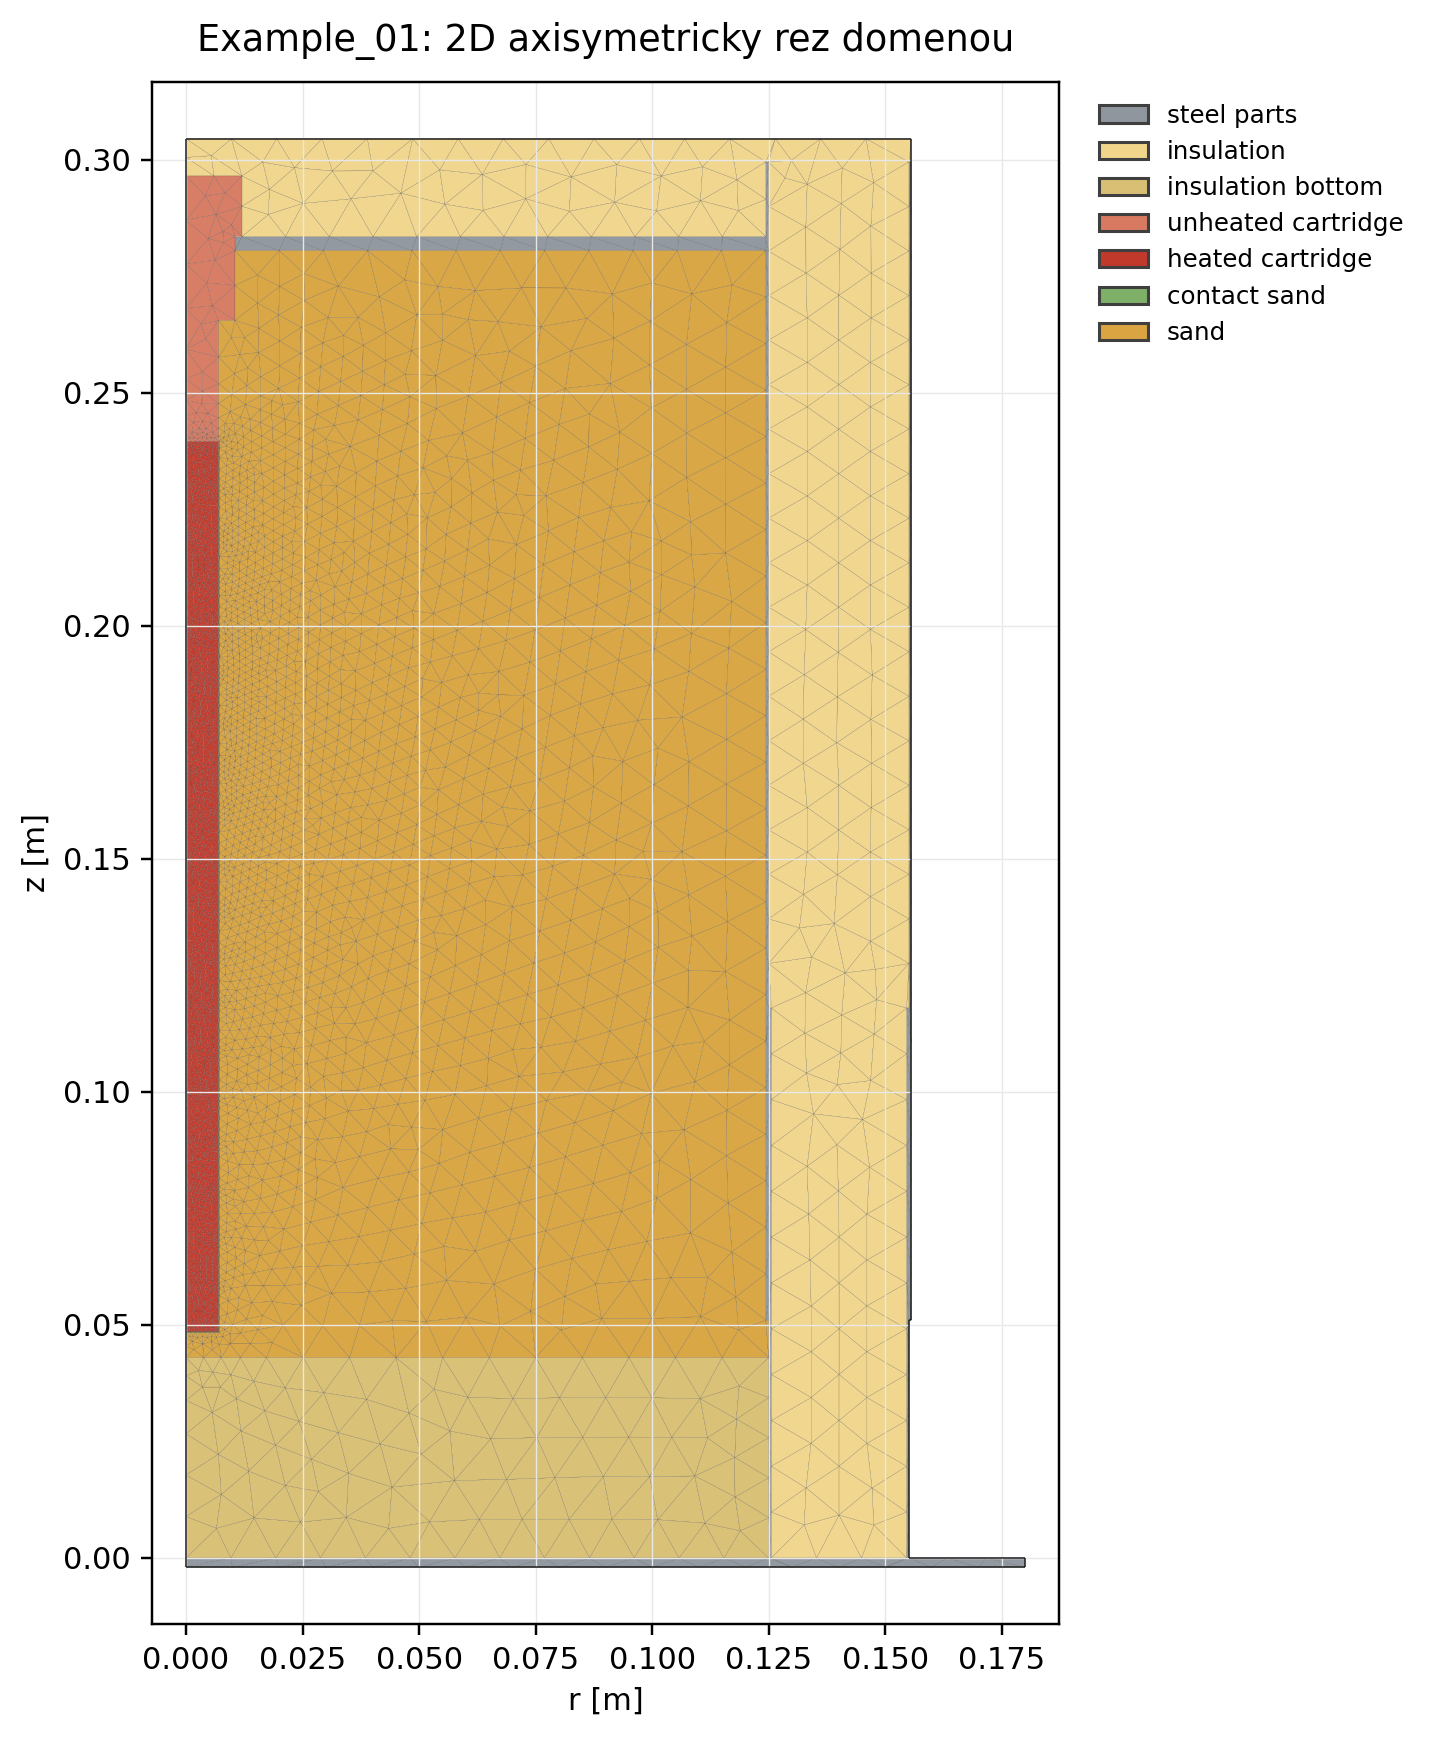
\includegraphics[width=0.82\linewidth]{images/example01-domain-paraview.png}
          \par\smallskip
          \small\emph{Example\_01: výpočtová doména a materiálové podoblasti.}
        \end{center}

        Stejný XDMF výstup lze otevřít v ParaView a zkontrolovat prostorové
        rozložení teploty v doméně. V řezu je dobře vidět lokální ohřev v okolí
        patrony a pomalejší šíření tepla do vzdálenějšího zásypu.

        \begin{center}
          {\setlength{\fboxsep}{0pt}\setlength{\fboxrule}{0.3pt}%
          \fbox{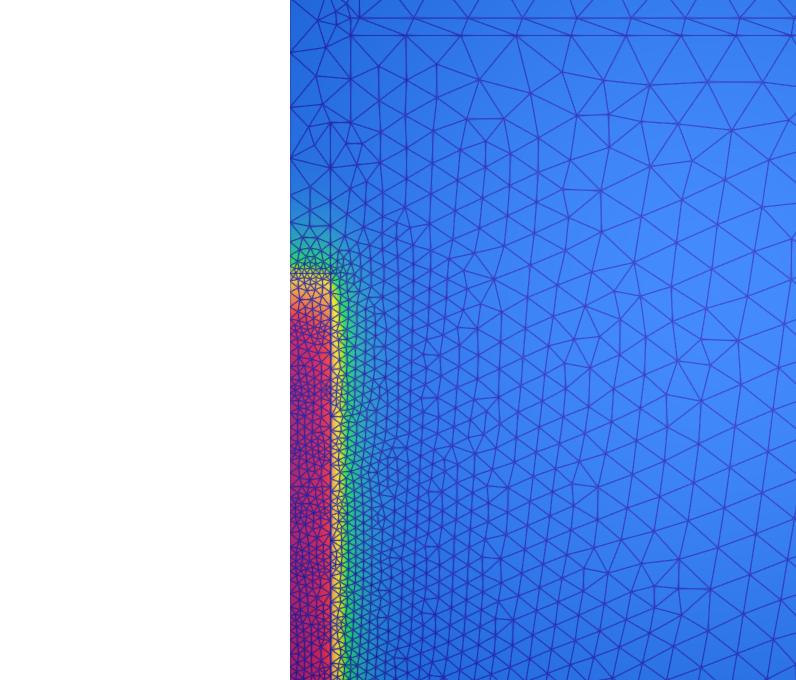
\includegraphics[width=0.82\linewidth]{images/example01-temperature-paraview.png}}}
          \par\smallskip
          \small\emph{Example\_01: teplotní pole z XDMF výstupu zobrazené v ParaView.}
        \end{center}

        Obrázek ukazuje základní odezvu modelu při krátkém nestacionárním běhu.
        Horní graf porovnává vybrané teplotní sondy, spodní graf ukazuje růst
        celkového uloženého tepla. Je na něm vidět, že nejrychleji reaguje
        oblast v okolí topné patrony, zatímco vzdálenější body zůstávají během
        krátkého běhu téměř na počáteční teplotě.

        \begin{center}
          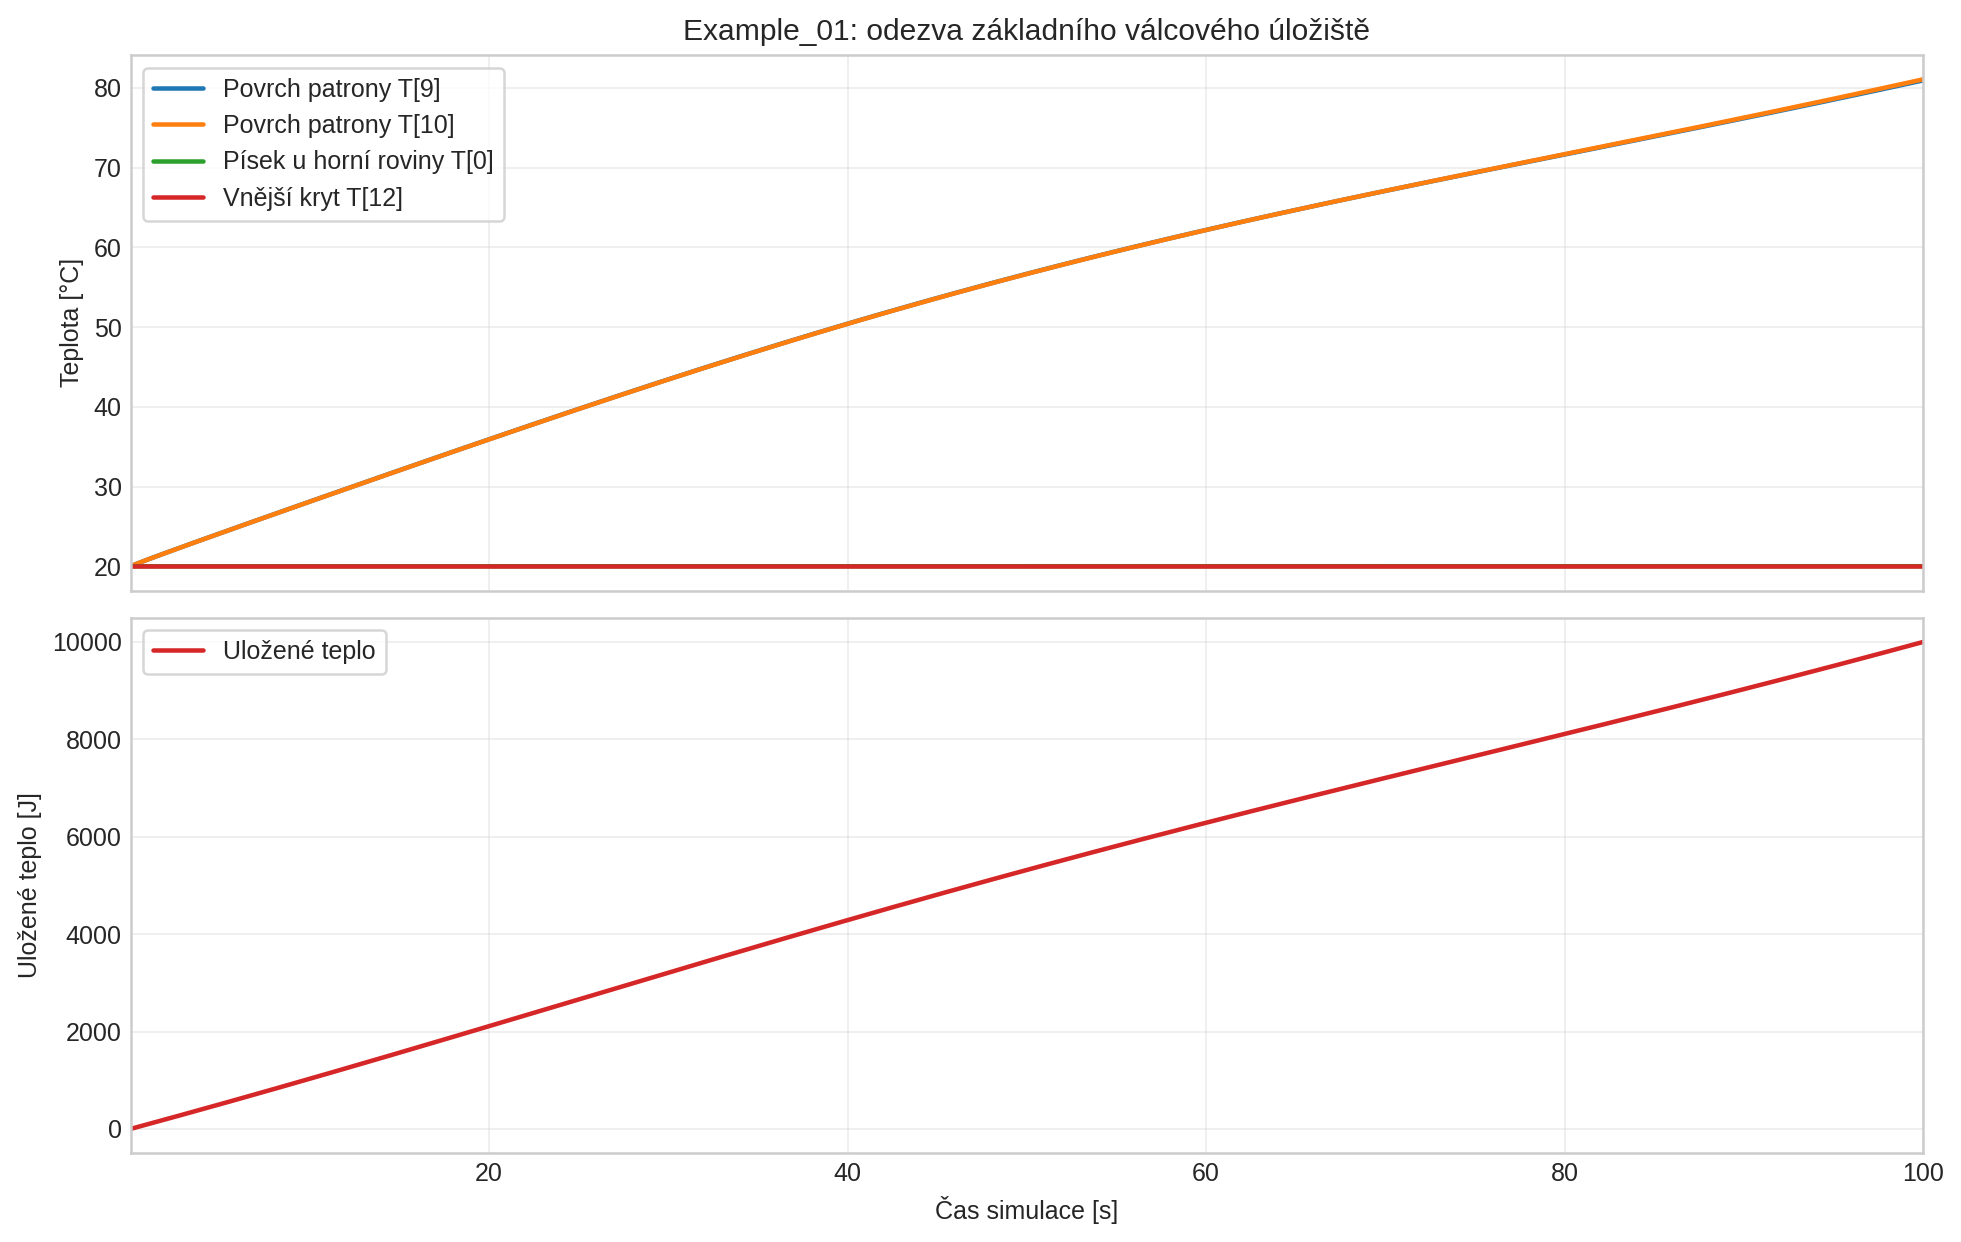
\includegraphics[width=0.92\linewidth]{images/example01-basic-response.png}
          \par\smallskip
          \small\emph{Example\_01: základní teplotní odezva a nárůst uloženého tepla.}
        \end{center}
  \item \textbf{Example\_02} -- fyzikálně shodný s Example\_01, ale
        \textbf{geometrie je importována ze STEP souboru} vytvořeného
        v CAD softwaru (Autodesk Inventor). Demonstruje cestu pro
        složitější geometrie, které není praktické skládat algoritmicky,
        a použití automatického \emph{extract\_axisymetry} z 3D modelu.
  \item \textbf{Example\_03} -- simulace metody \emph{transient hot wire}
        (THW) pro měření tepelné vodivosti zásypu. V geometrii dvoudrátové
        sondy se počítá časový vývoj odporu obou tantalových vláken
        (proudově buzených konstantním výkonem), z něhož se přes
        Wheatstoneův můstek dopočítává tepelná vodivost. Příklad pokrývá
        nelineární zdrojový člen závislý na teplotě a post-processing CSV
        výstupu.

        Obrázek ukazuje typický výstup z post-processingu tohoto příkladu.
        Horní graf zobrazuje nárůst teploty v čase. Teplota odvozená z odporu
        vodiče se prakticky překrývá s bodovou MKP sondou v místě vodiče; tím se
        ověřuje, že odporový Term, odečet teploty i následný post-processing
        dávají konzistentní výsledek. Spodní graf ukazuje odhad tepelné
        vodivosti
        \[
          \lambda = \frac{q_l}{4\pi\,\mathrm{d}T/\mathrm{d}\ln t},
        \]
        kde \(q_l\) je délkový tepelný výkon vodiče. Logaritmická osa času
        odpovídá způsobu, jakým se data z transient hot-wire měření obvykle
        vyhodnocují. Tepelná vodivost je vyčítána v okamžiku kde je průběh
        odporové sondy v logaritmickém měřítku lineární.
        \begin{center}
          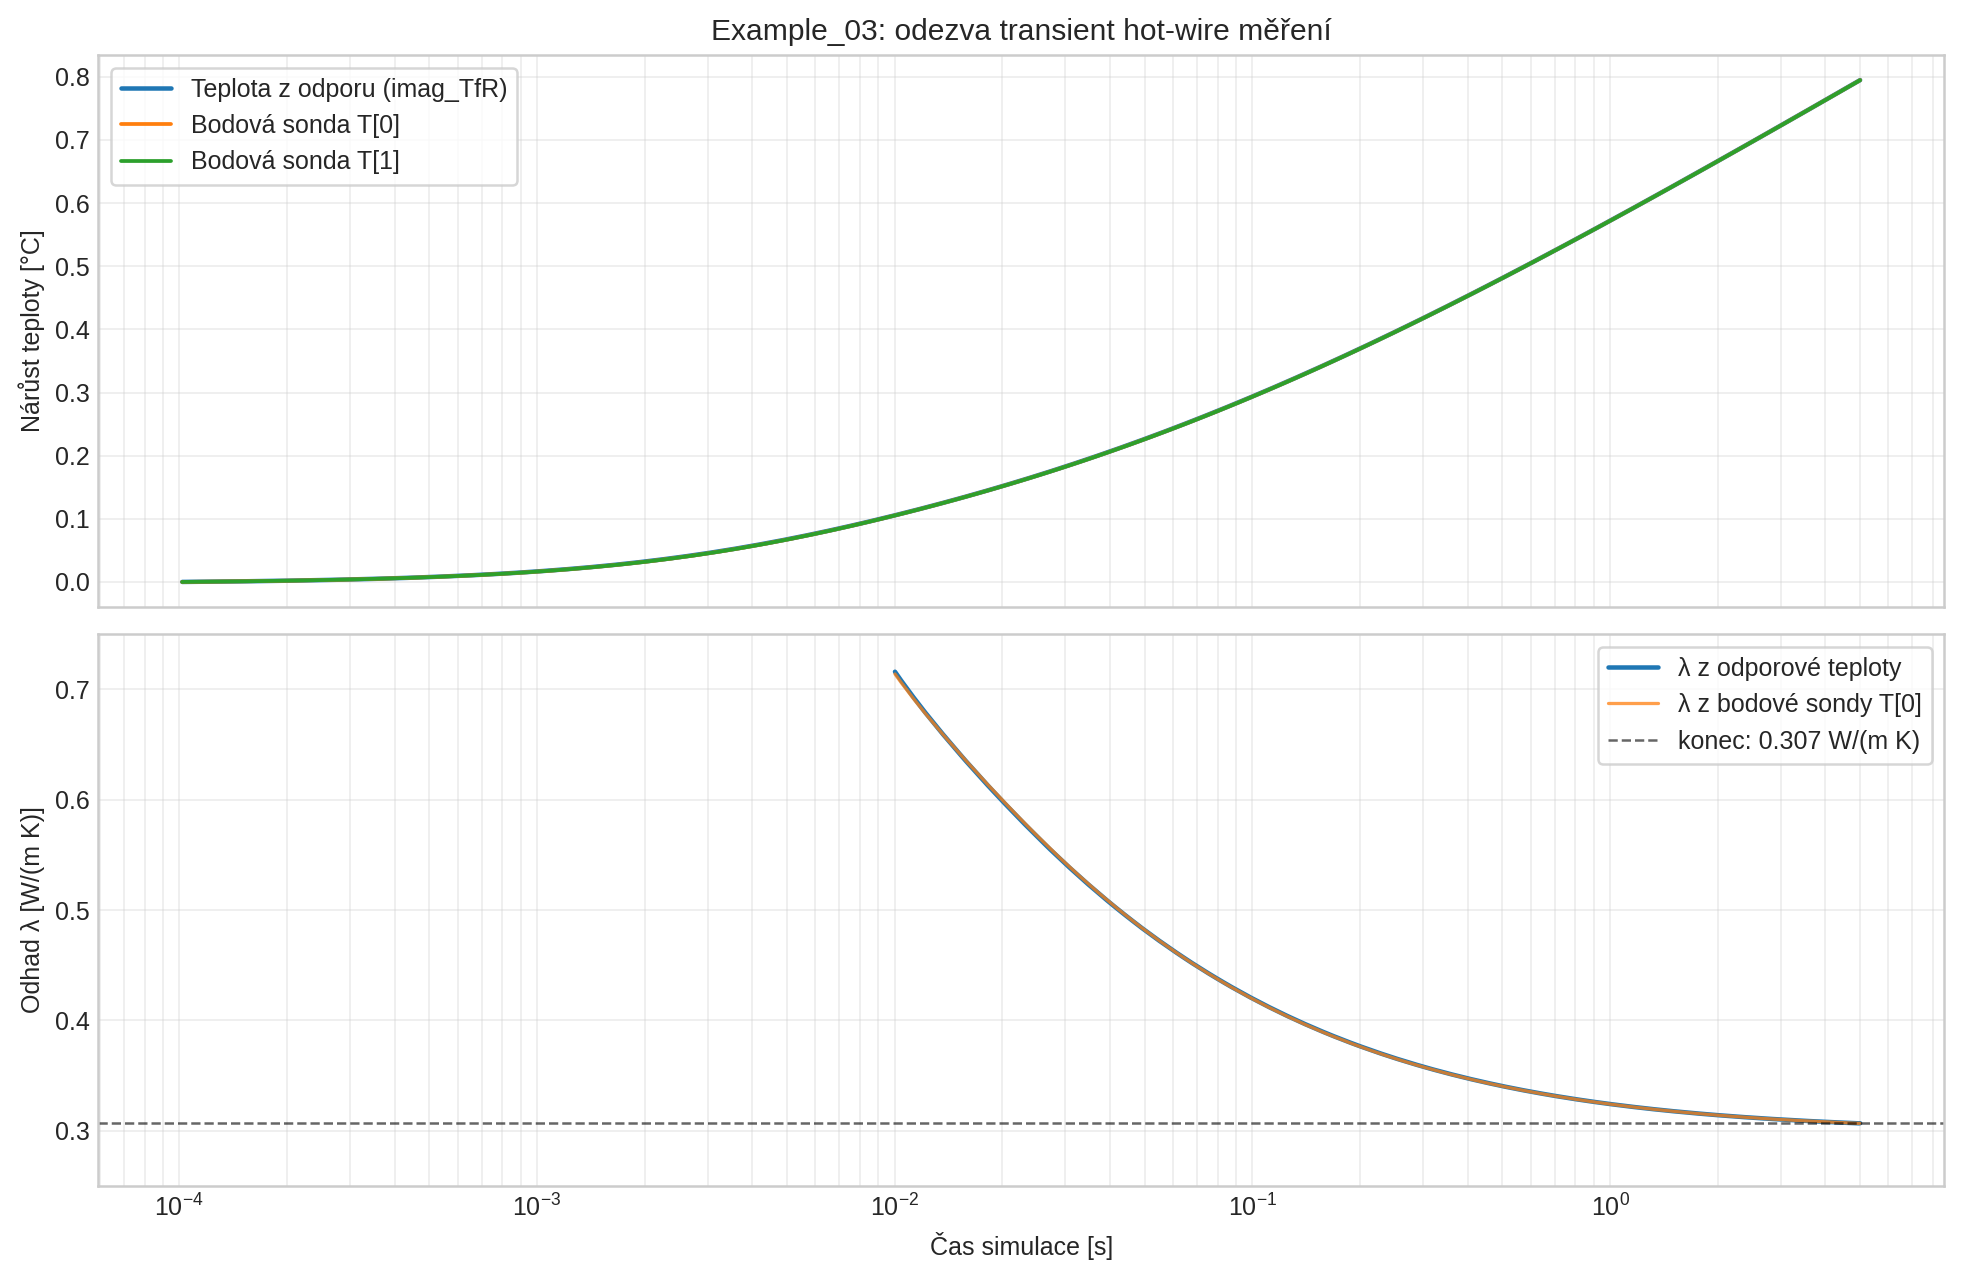
\includegraphics[width=0.92\linewidth]{images/example03-thw-response.png}
          \par\smallskip
          \small\emph{Example\_03: odezva transient hot-wire měření a odhad tepelné vodivosti.}
        \end{center}
  \item \textbf{Example\_04} -- pasivní úložiště s \textbf{PID-řízenou
        topnou patronou}. Geometrie je importována ze STEP
        (\texttt{Passive\_storage.stp}), regulátor řídí výkon patrony tak,
        aby průměrná teplota povrchu patrony sledovala zadanou referenci
        (výchozí hodnota \(400\,^\circ\mathrm{C}\)). Demonstruje použití termu
        \texttt{PIDControlled\allowbreak HeatSource}, který má vlastní vnější iterační
        smyčku (\texttt{converged} / \texttt{adaptation}) zajišťující
        implicitní vazbu mezi teplotou a akčním zásahem.

        Obrázek níže ukazuje detail prvních čtyř hodin běhu. Tento rozsah je
        zvolený proto, aby byl dobře vidět náběh PID regulace: průměrná teplota
        povrchu patrony \texttt{Tc\_avg} se rychle přiblíží k referenci
        \(400\,^\circ\mathrm{C}\), zatímco teploty v tělese úložiště a na
        okrajových površích se v tomto krátkém čase téměř nemění.

        \begin{center}
          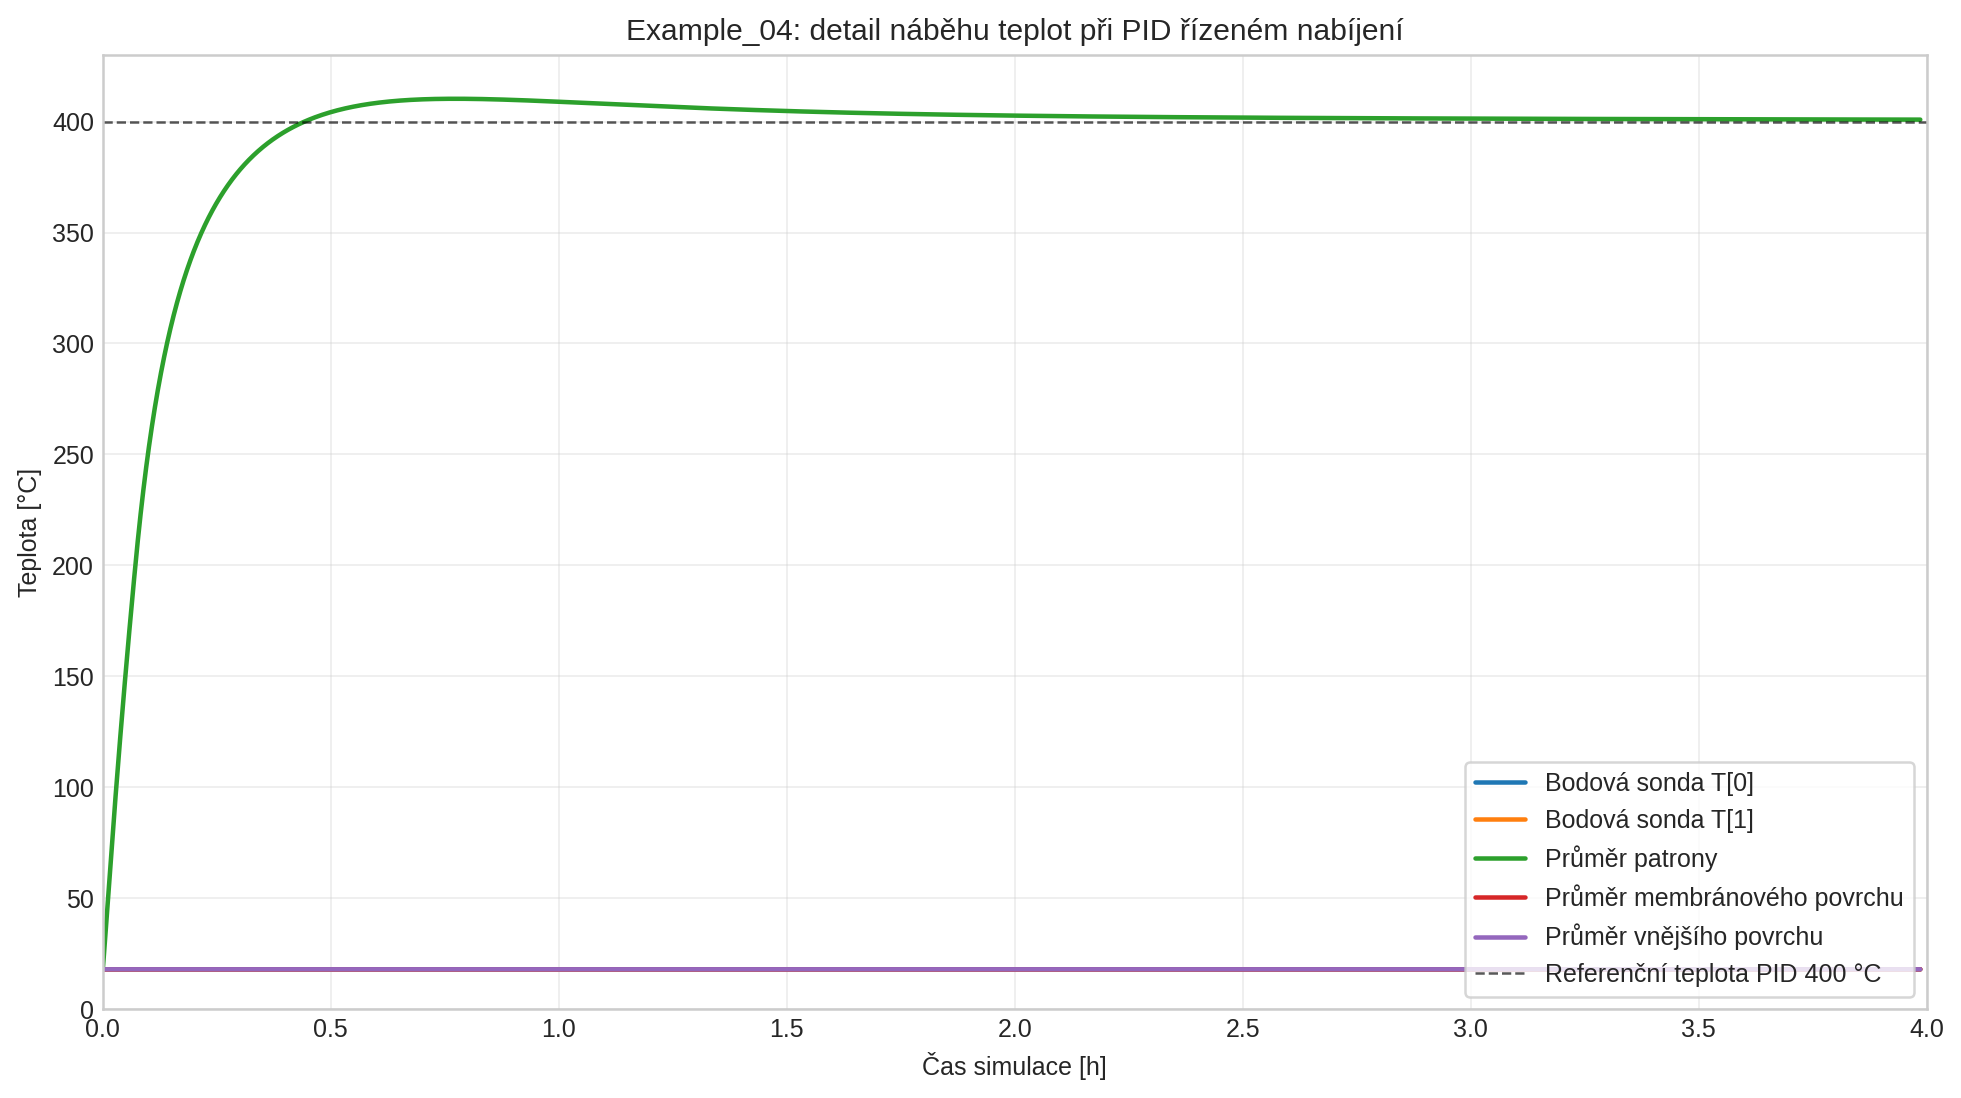
\includegraphics[width=0.92\linewidth]{images/example04-temperature-course.png}
          \par\smallskip
          \small\emph{Example\_04: detail náběhu teplot při PID řízeném nabíjení topné patrony.}
        \end{center}
  \item \textbf{Example\_05} -- simulace tepelného zásobníku nabíjeného
        z FVE, který dodává teplo do výrobní haly (Hala C3 FSI VUT Brno).
        Obsahuje plnohodnotnou \textbf{ko-simulaci se zjednodušeným modelem haly}
        (HallC3), čerpání meteorologických dat z PVGIS (NSRDB),
        ekvitermní regulaci a bivalentní záložní zdroj.
        \textbf{Parametrická studie} (\texttt{ParameterGrid}) prochází
        hlavní rozměry úložiště a topidel na dvou letech provozu;
        jednotlivé kombinace se distribuují přes PostgreSQL frontu a MPI workery.
        Jde o nejkomplexnější příklad v repozitáři: využívá téměř všechny hlavní
        moduly balíčku, od geometrie a meteorologických dat přes termy,
        ko-simulaci, sondy a databázový projekt až po webovou vizualizaci.
        Jeho výsledky, včetně obrázků webového rozhraní, jsou uvedeny
        v následující podkapitole.
  \item \textbf{Example\_06} -- jednodušší varianta Example\_05 použitá
        pro \textbf{validaci checkpoint mechanismu} (běh napřímo, bez
        databáze). Stejný model spustí třikrát: jednou souvisle, jednou
        s uloženým checkpointem v polovině a jednou pokračováním z toho
        checkpointu -- výsledné sondy \(Q_\mathrm{amb}\) musí být
        v rámci tolerance shodné, čímž se ověří úplnost serializace
        stavu (DoFs, konstanty termů, \(T_n\), délka CSV souboru, režim XDMF).
\end{itemize}

V každém adresáři \path{examples/Example_*/} jsou kromě README také soubory
\path{geometry*.py}, \texttt{model.py} a \path{run_example*.py}; dohromady tvoří
kompletní postup od geometrie a sítě až po výstupy. Většinu příkladů lze spustit
jedním příkazem, například:

\begin{lstlisting}[style=bash]
mpirun -n 4 python3 -m examples.Example_xx.run_example
\end{lstlisting}

\subsection*{Ukázky výsledků z Example\_05}

Následující obrázky jsou přímo z webového rozhraní nad PostgreSQL projektem
\textbf{Example\_05}. Ukazují, jak se výsledky parametrické studie čtou v praxi:
nejdříve se v tabulce vybere konkrétní úloha, potom se v prohlížeči výsledků
zobrazí časové průběhy sond. Pro ukázku jsou vybrány konfigurace s různou
velikostí akumulátoru a různým počtem topných patron, protože právě tyto
parametry výrazně ovlivňují schopnost systému přijmout výkon z FVE.

\begin{figure}[H]
  \centering
  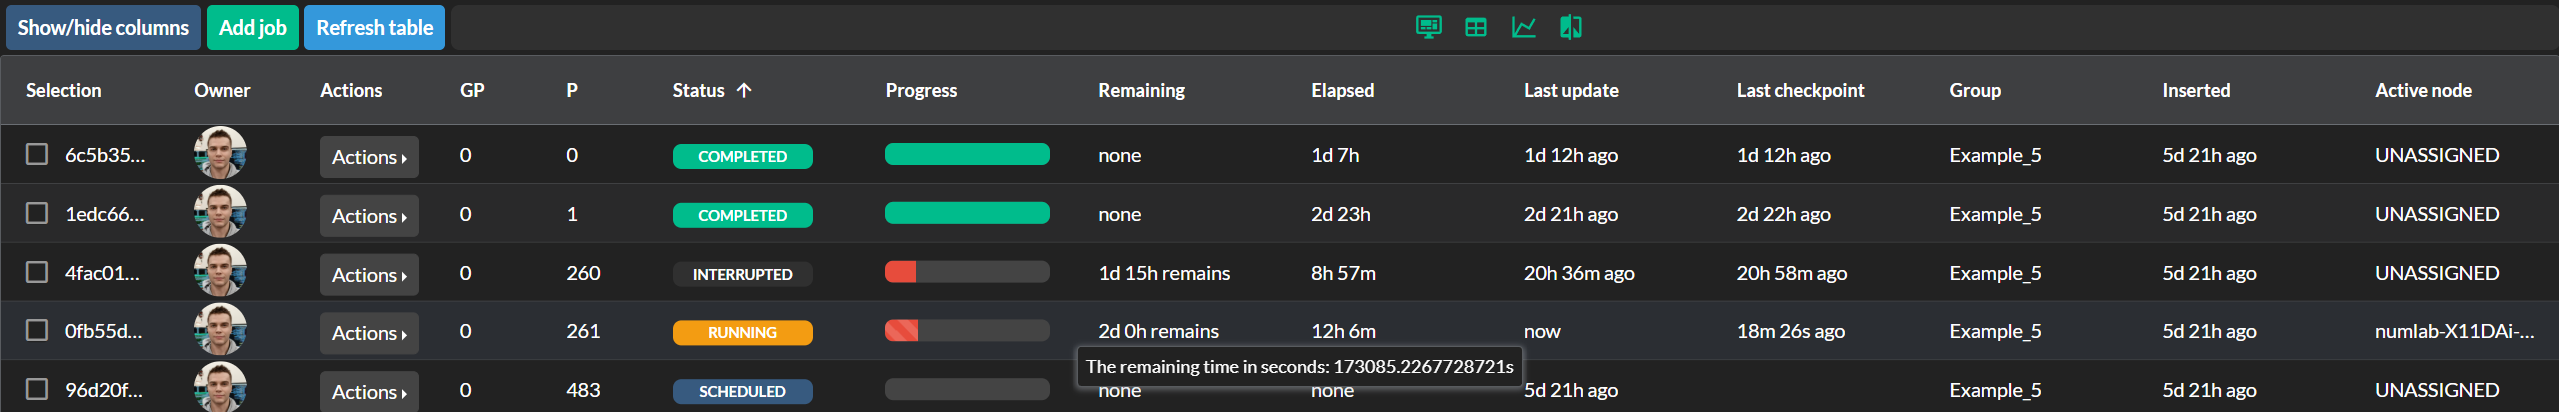
\includegraphics[width=0.98\linewidth]{example_5_result_images/table_detail.png}
  \caption{Tabulka úloh v dashboardu. Sloupce \texttt{P} a \texttt{Status}
           umožňují rychle najít dokončené, běžící nebo přerušené simulace;
           zvolenou úlohu lze otevřít v prohlížeči výsledků.}
  \label{fig:c3-table}
\end{figure}

Souhrnný pohled pro malý akumulátor o průměru a výšce přibližně
\(1 \times 1\,\mathrm{m}\) ukazuje všechny hlavní skupiny veličin najednou:
teploty v akumulátoru, tepelné toky, celkovou energii, účinnosti a chování
nelineárního řešiče. Takový přehled je vhodný pro první kontrolu, zda simulace
doběhla fyzikálně smysluplně, zda nedochází k přehřívání topidel a zda solver
nemá v některých obdobích výrazně vyšší počet iterací.

\begin{figure}[H]
  \centering
  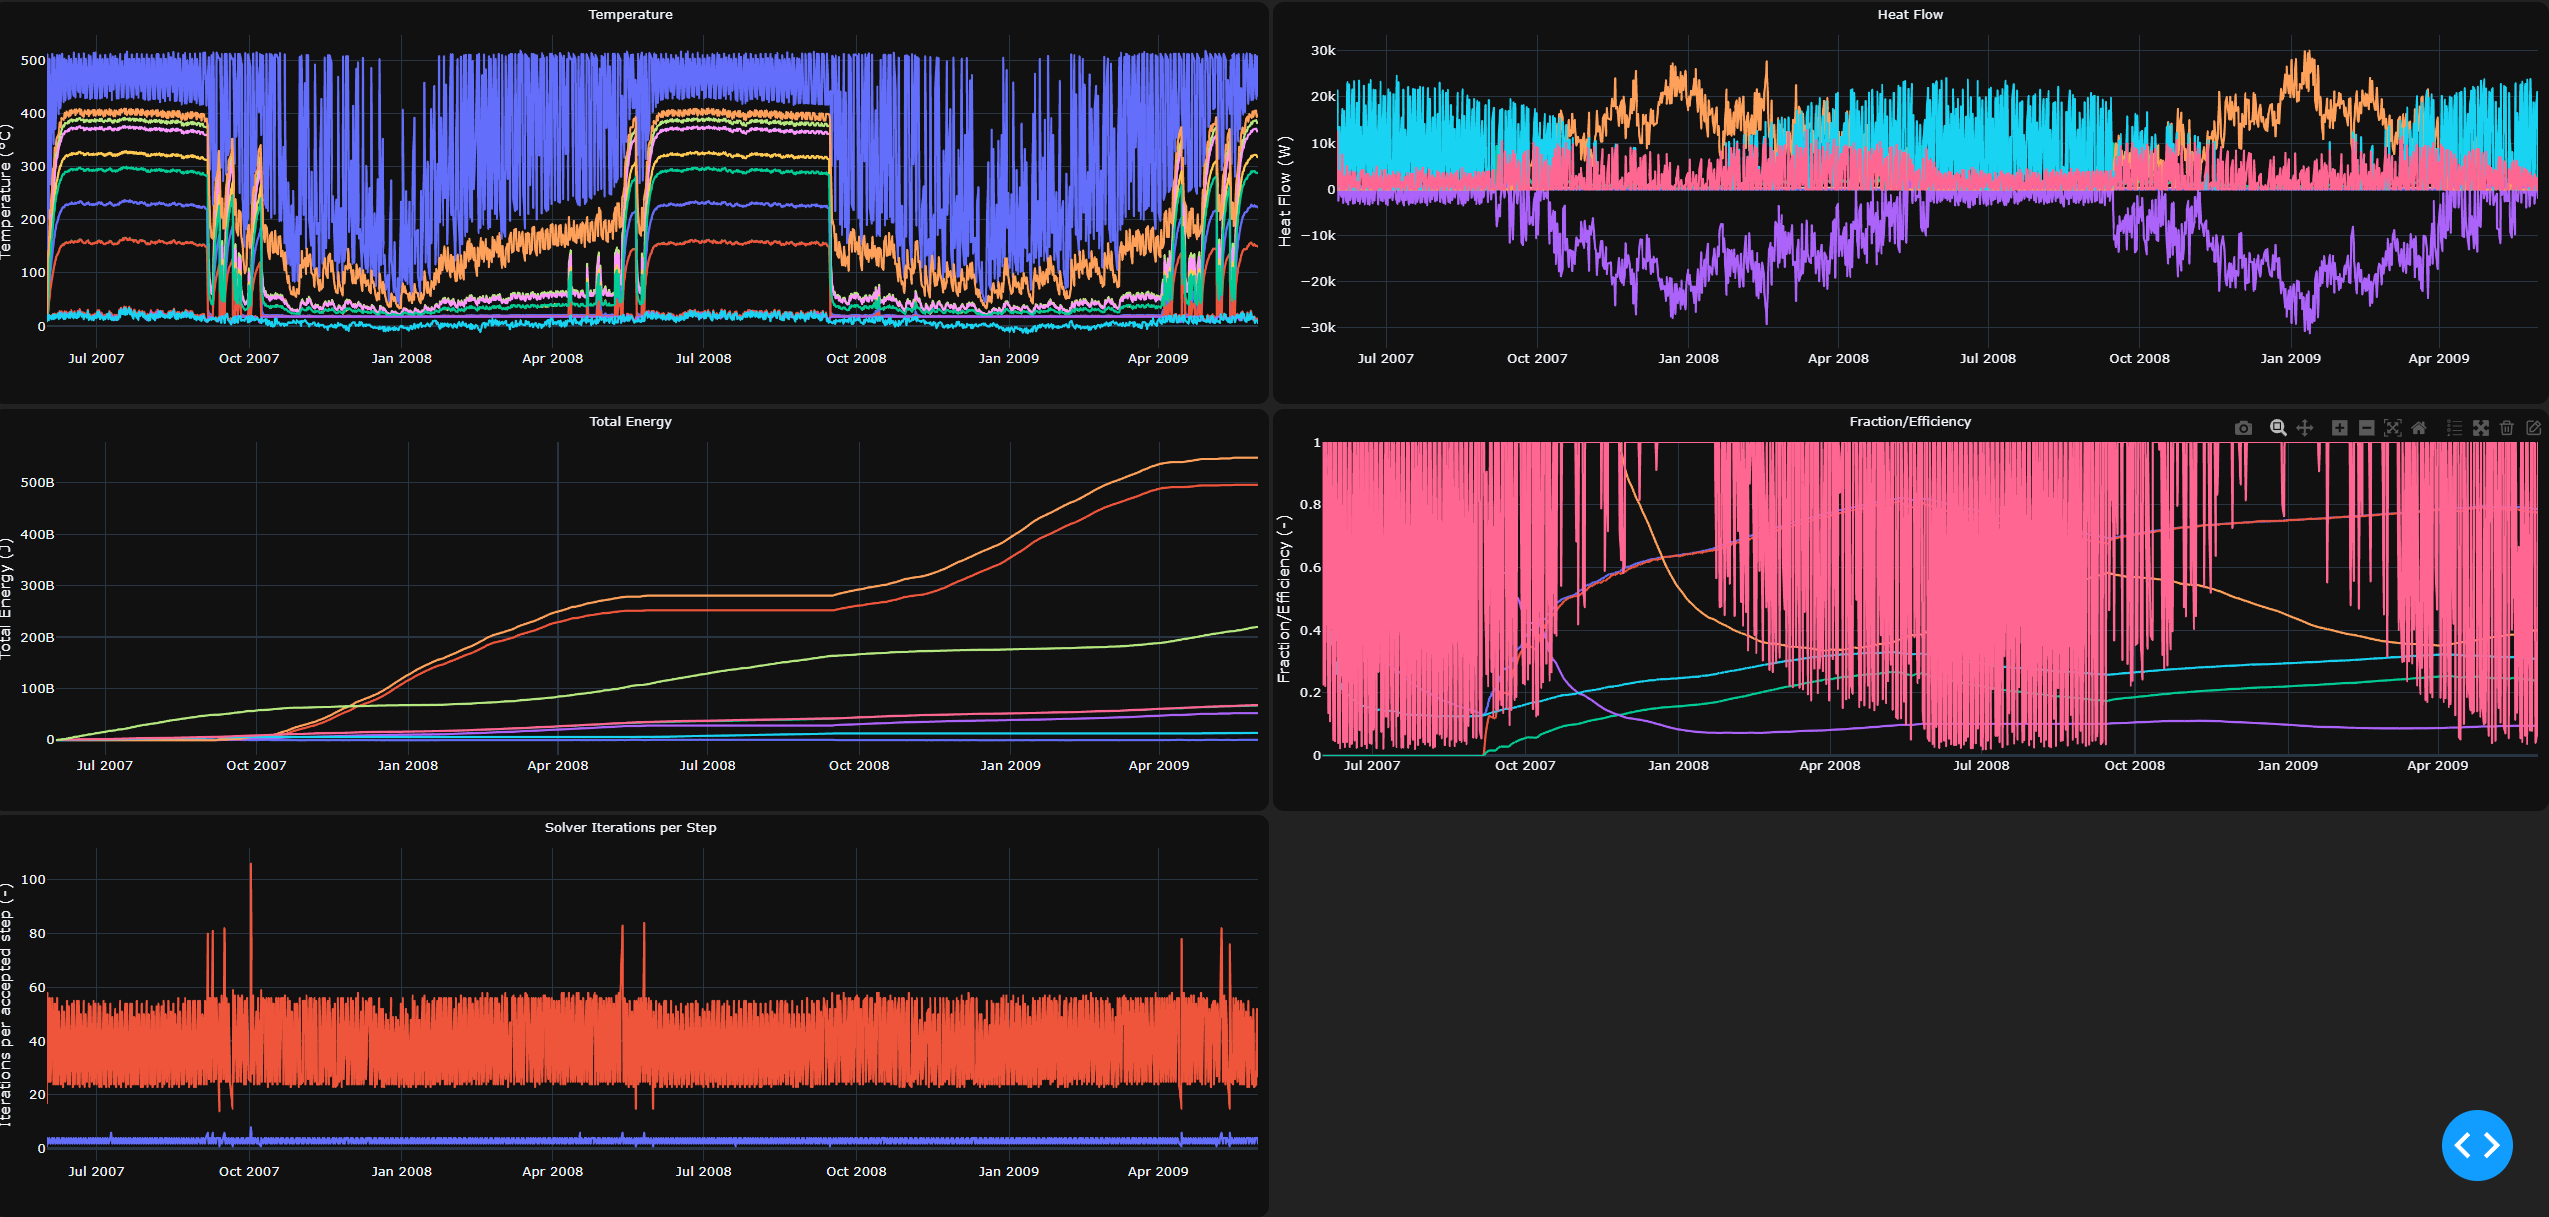
\includegraphics[width=0.98\linewidth]{example_5_result_images/size1-all_charts.png}
  \caption{Dashboard pro malý akumulátor \(1 \times 1\,\mathrm{m}\): teploty,
           toky, energie, účinnosti a iterace řešiče v jednom souhrnném pohledu.}
  \label{fig:c3-size1-all}
\end{figure}

Detail teplot pro malý akumulátor o průměru a výšce přibližně \(1 \times 1\,\mathrm{m}\)
se čtyřmi patronami ukazuje rychlý ohřev topných elementů až k hornímu
teplotnímu omezení. Vnitřní sondy reagují pozvolněji, protože teplo se ze zdrojů
šíří do zásypu postupně. Tento případ je vhodný pro kontrolu ochrany topidel
a vazby mezi dostupným výkonem z FVE, Termem topné patrony a teplotními sondami
v zásobníku.

\begin{figure}[H]
  \centering
  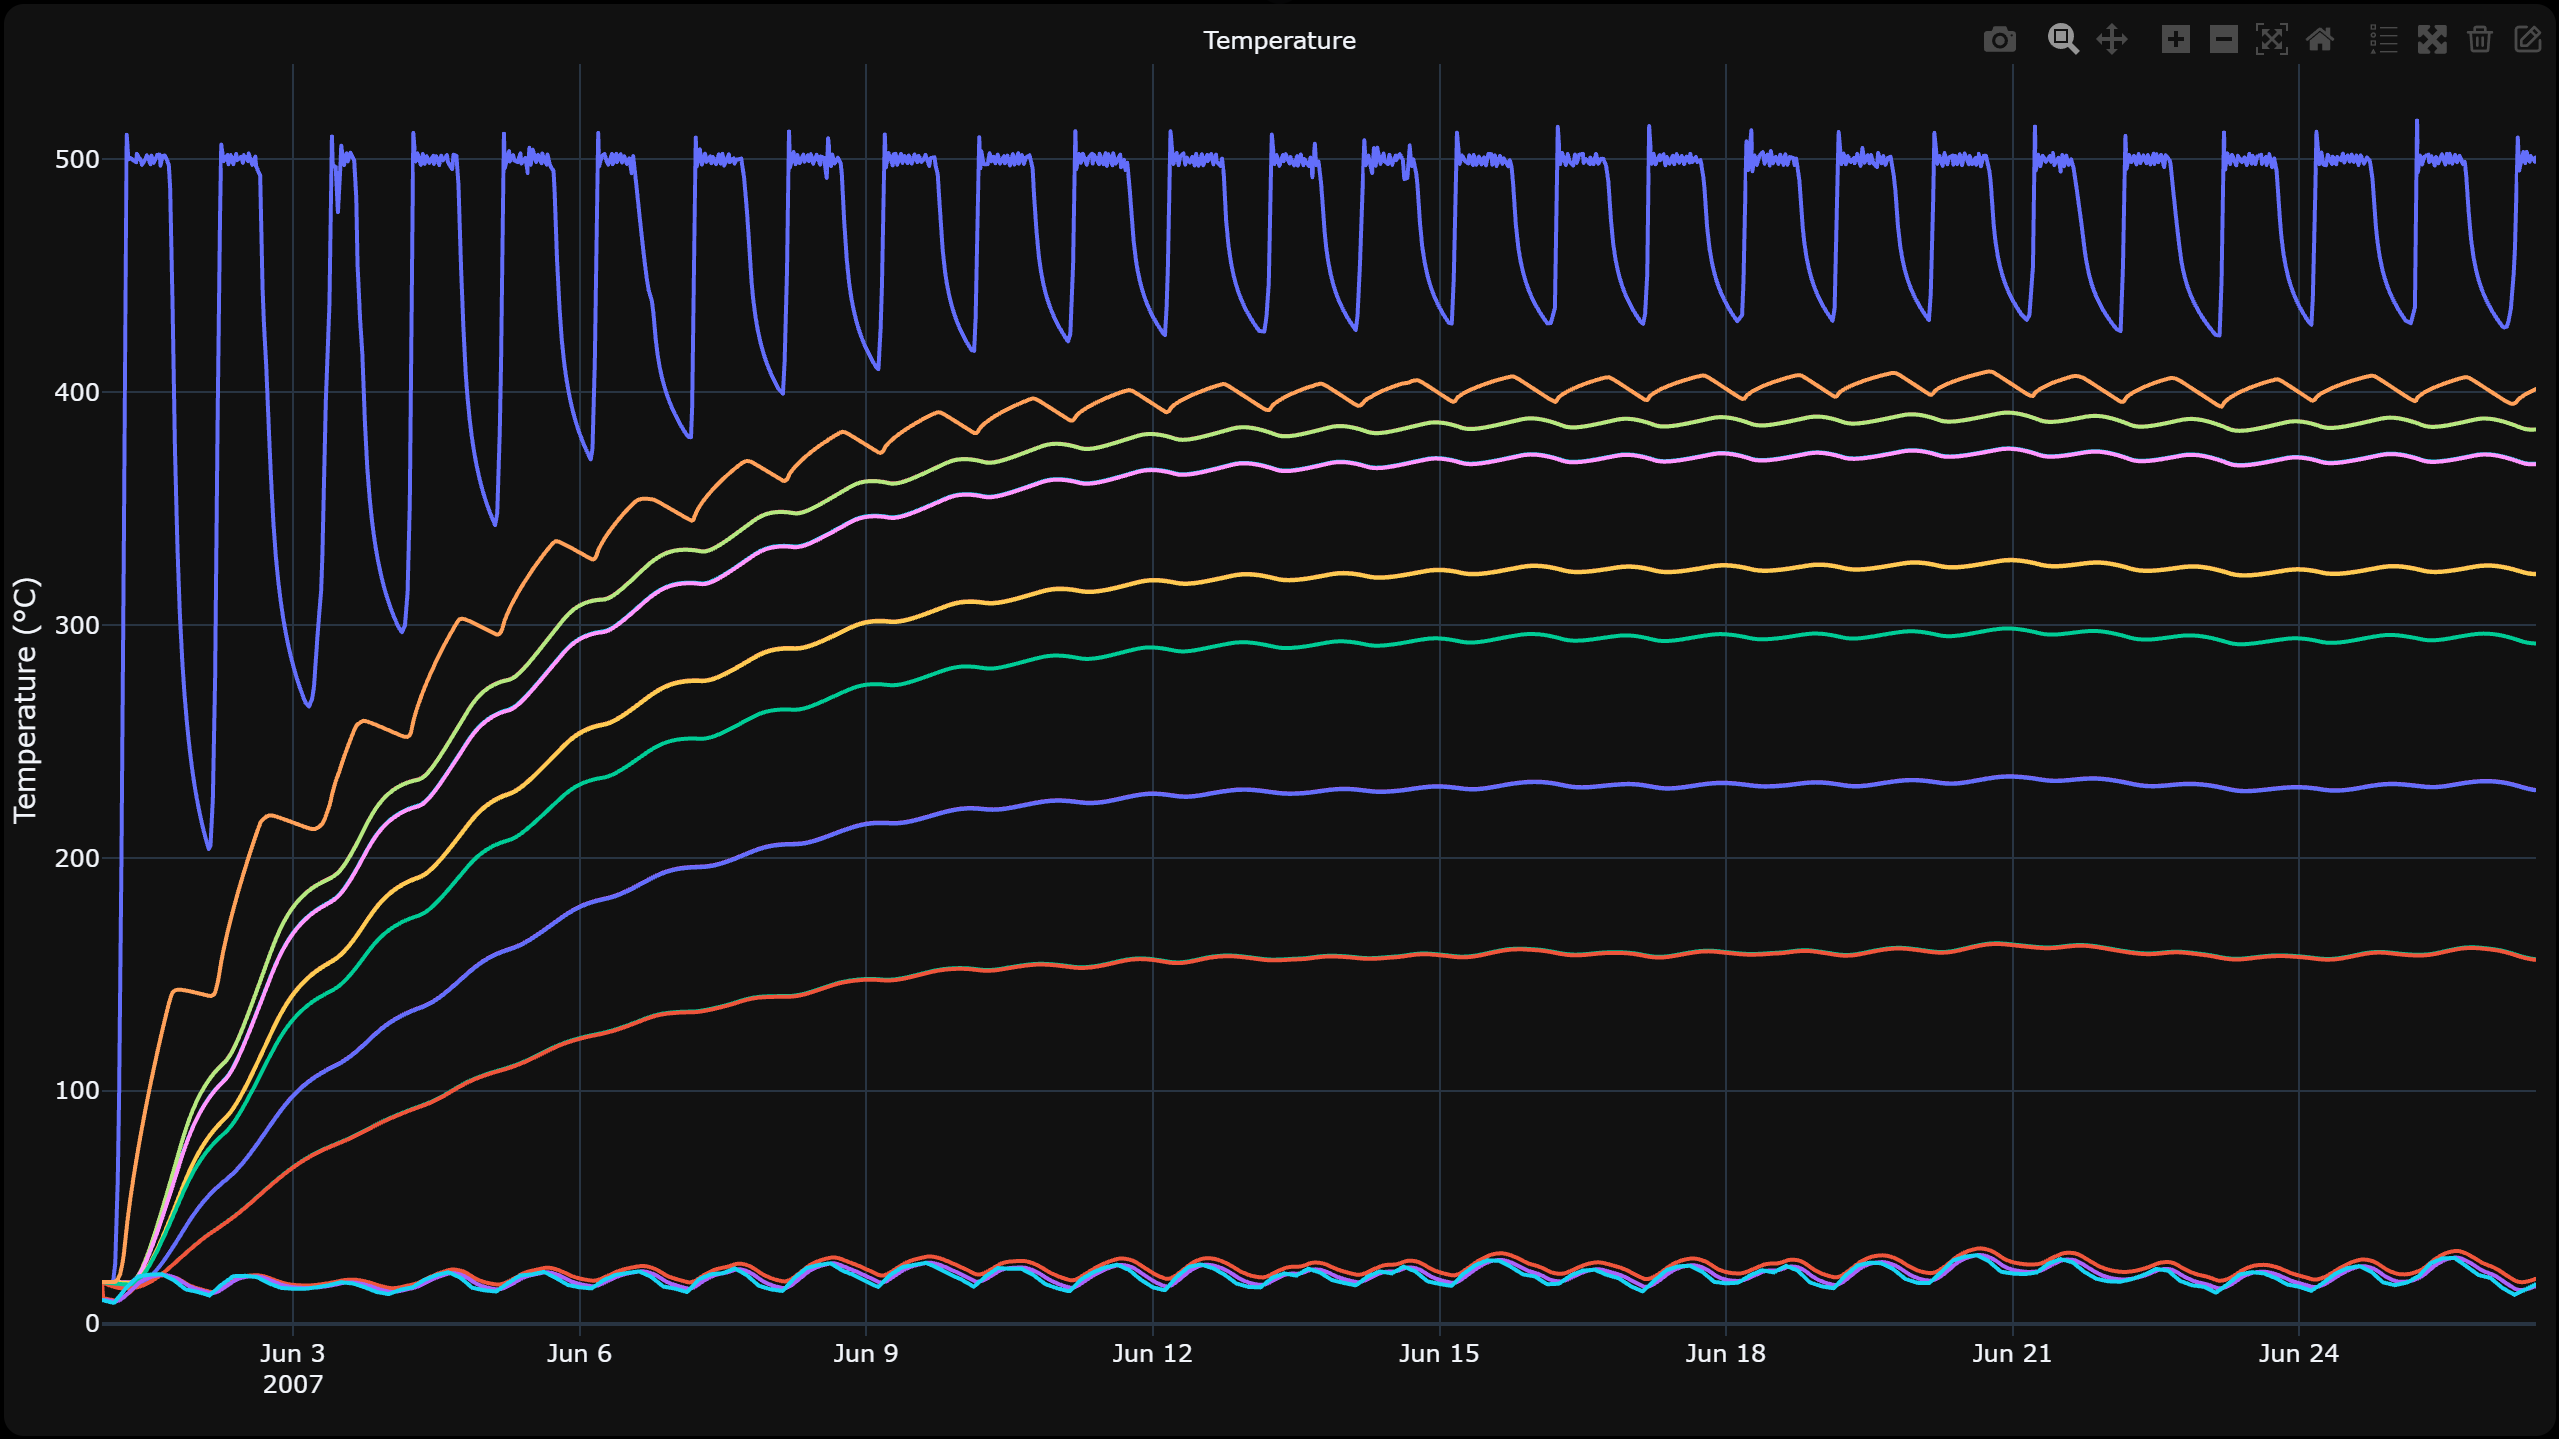
\includegraphics[width=0.98\linewidth]{example_5_result_images/size1-4cartridges.png}
  \caption{Malý akumulátor \(1 \times 1\,\mathrm{m}\) se čtyřmi patronami:
           rychlý ohřev topidel a postupné nabíjení teplotních sond uvnitř
           akumulátoru.}
  \label{fig:c3-size1-4}
\end{figure}

Porovnání akumulátoru o průměru a výšce přibližně \(3 \times 3\,\mathrm{m}\)
ukazuje vliv počtu topných patron. Při čtyřech patronách se lokální teplota
topidel často blíží limitu, zatímco zbytek akumulátoru se ohřívá pomalu.
Po zvýšení počtu patron na deset se stejný vstupní výkon rozloží do většího
objemu: teplotní špičky jsou nižší a nabíjení je rovnoměrnější. Tato dvojice
obrázků dobře ukazuje, proč nestačí navrhovat jen celkovou kapacitu zásobníku;
důležité je i prostorové rozložení zdrojů tepla.

\begin{figure}[H]
  \centering
  \begin{minipage}{0.49\linewidth}
    \centering
    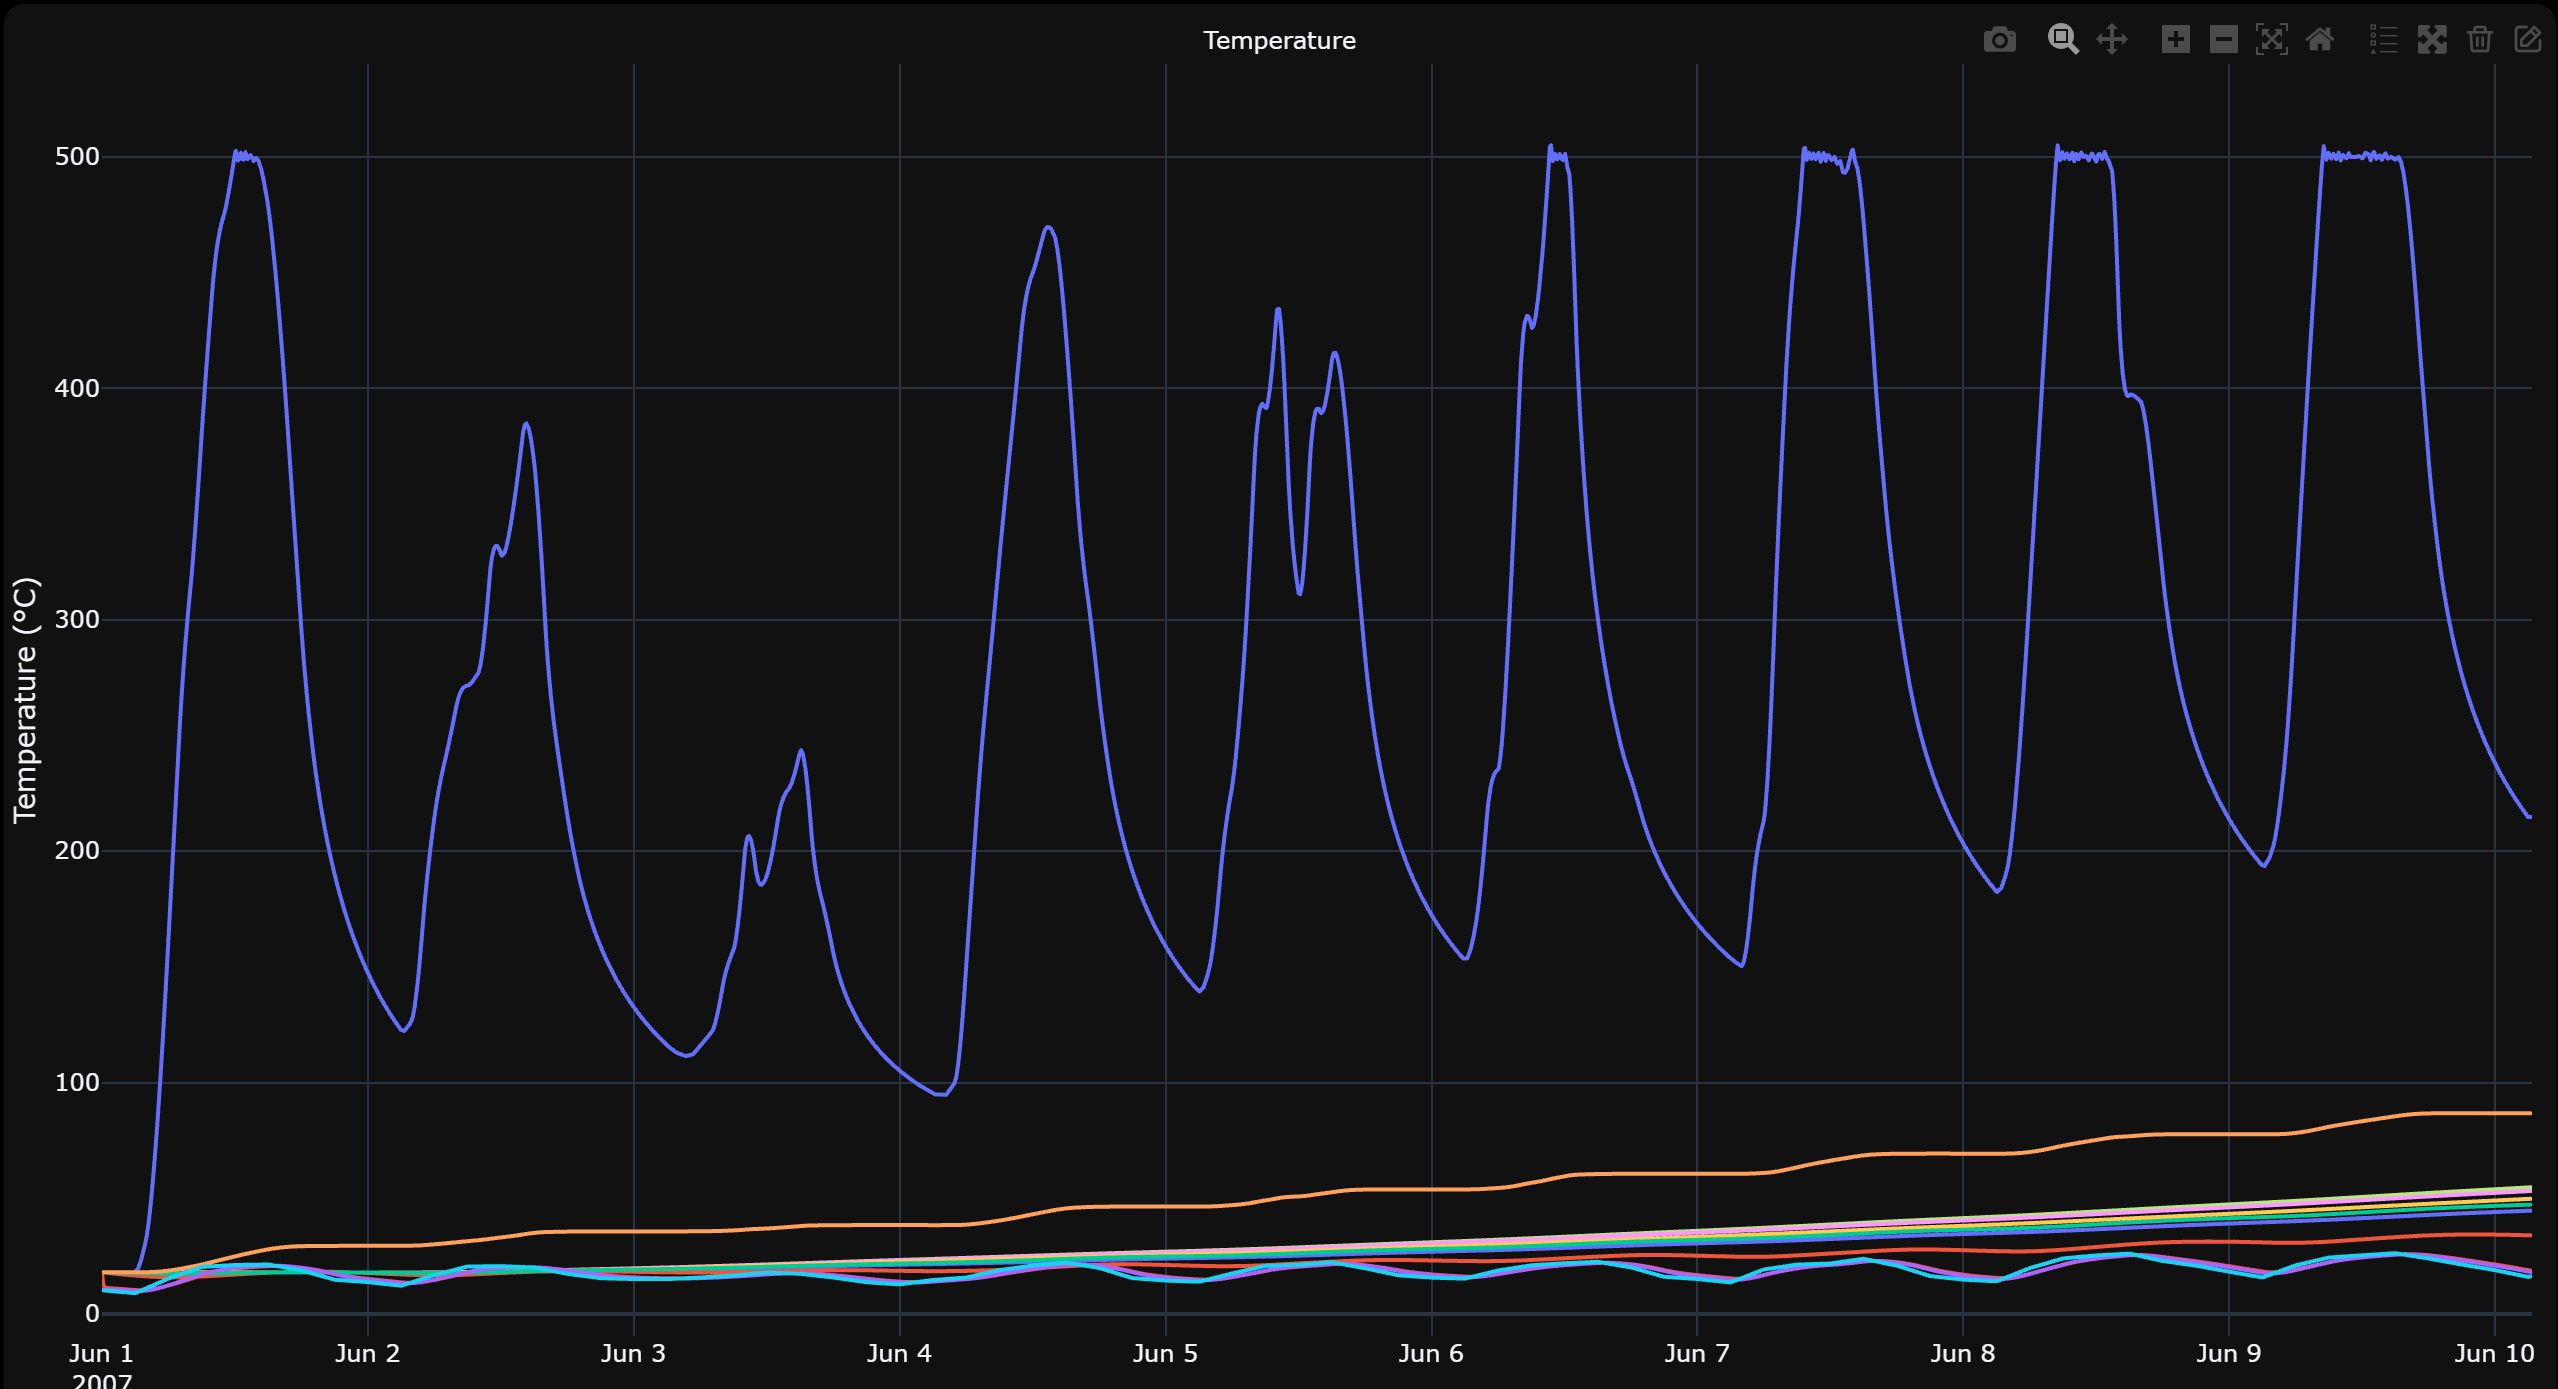
\includegraphics[width=\linewidth]{example_5_result_images/size3-4cartridges.png}
  \end{minipage}
  \hfill
  \begin{minipage}{0.49\linewidth}
    \centering
    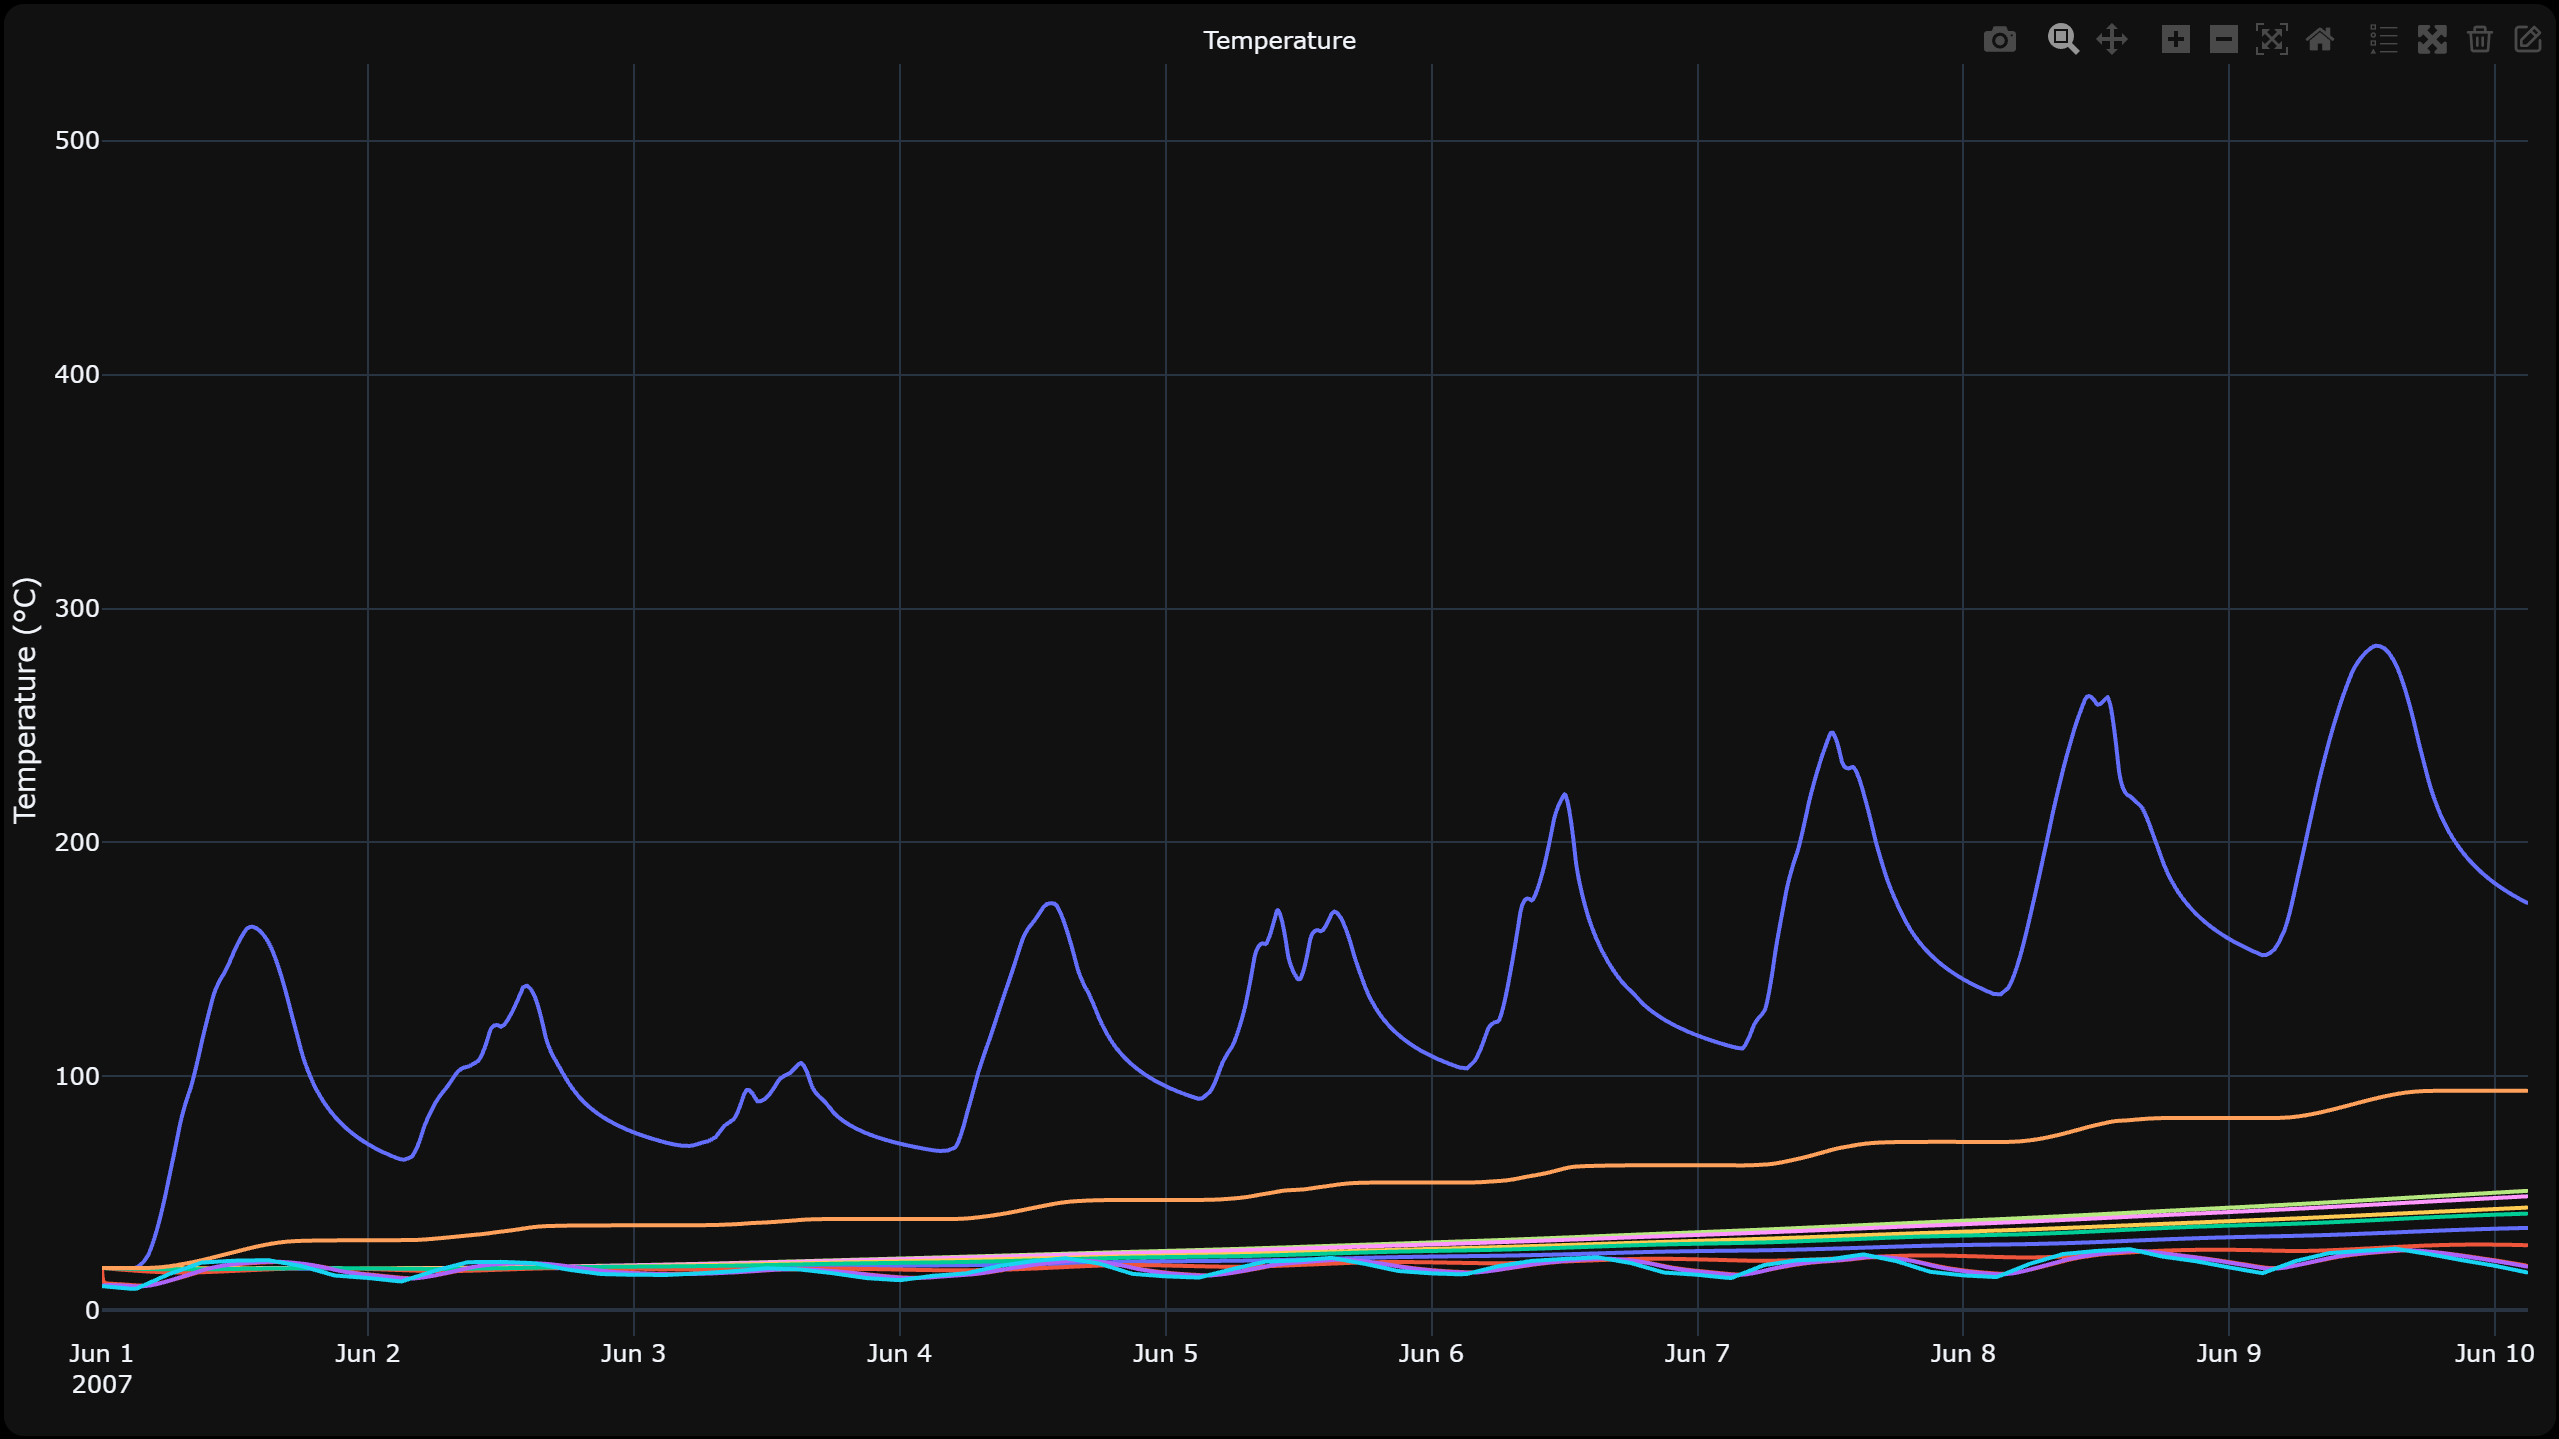
\includegraphics[width=\linewidth]{example_5_result_images/size3-10cartridges.png}
  \end{minipage}
  \caption{Akumulátor \(3 \times 3\,\mathrm{m}\): vlevo čtyři patrony
           s výraznými lokálními špičkami, vpravo deset patron s rovnoměrnějším
           rozložením výkonu.}
  \label{fig:c3-size3-comparison}
\end{figure}

Velký akumulátor o průměru a výšce přibližně \(5 \times 5\,\mathrm{m}\)
s deseti patronami se chová jinak: neukazuje jen krátkodobé denní cykly, ale
také sezónní nabíjení a vybíjení. V létě roste teplota větší části zásobníku,
v zimě se akumulátor postupně vybíjí do haly. Detail prvního měsíce lépe
ukazuje denní pulzy od FVE a pomalé zvyšování teploty hmoty akumulátoru.

\begin{figure}[H]
  \centering
  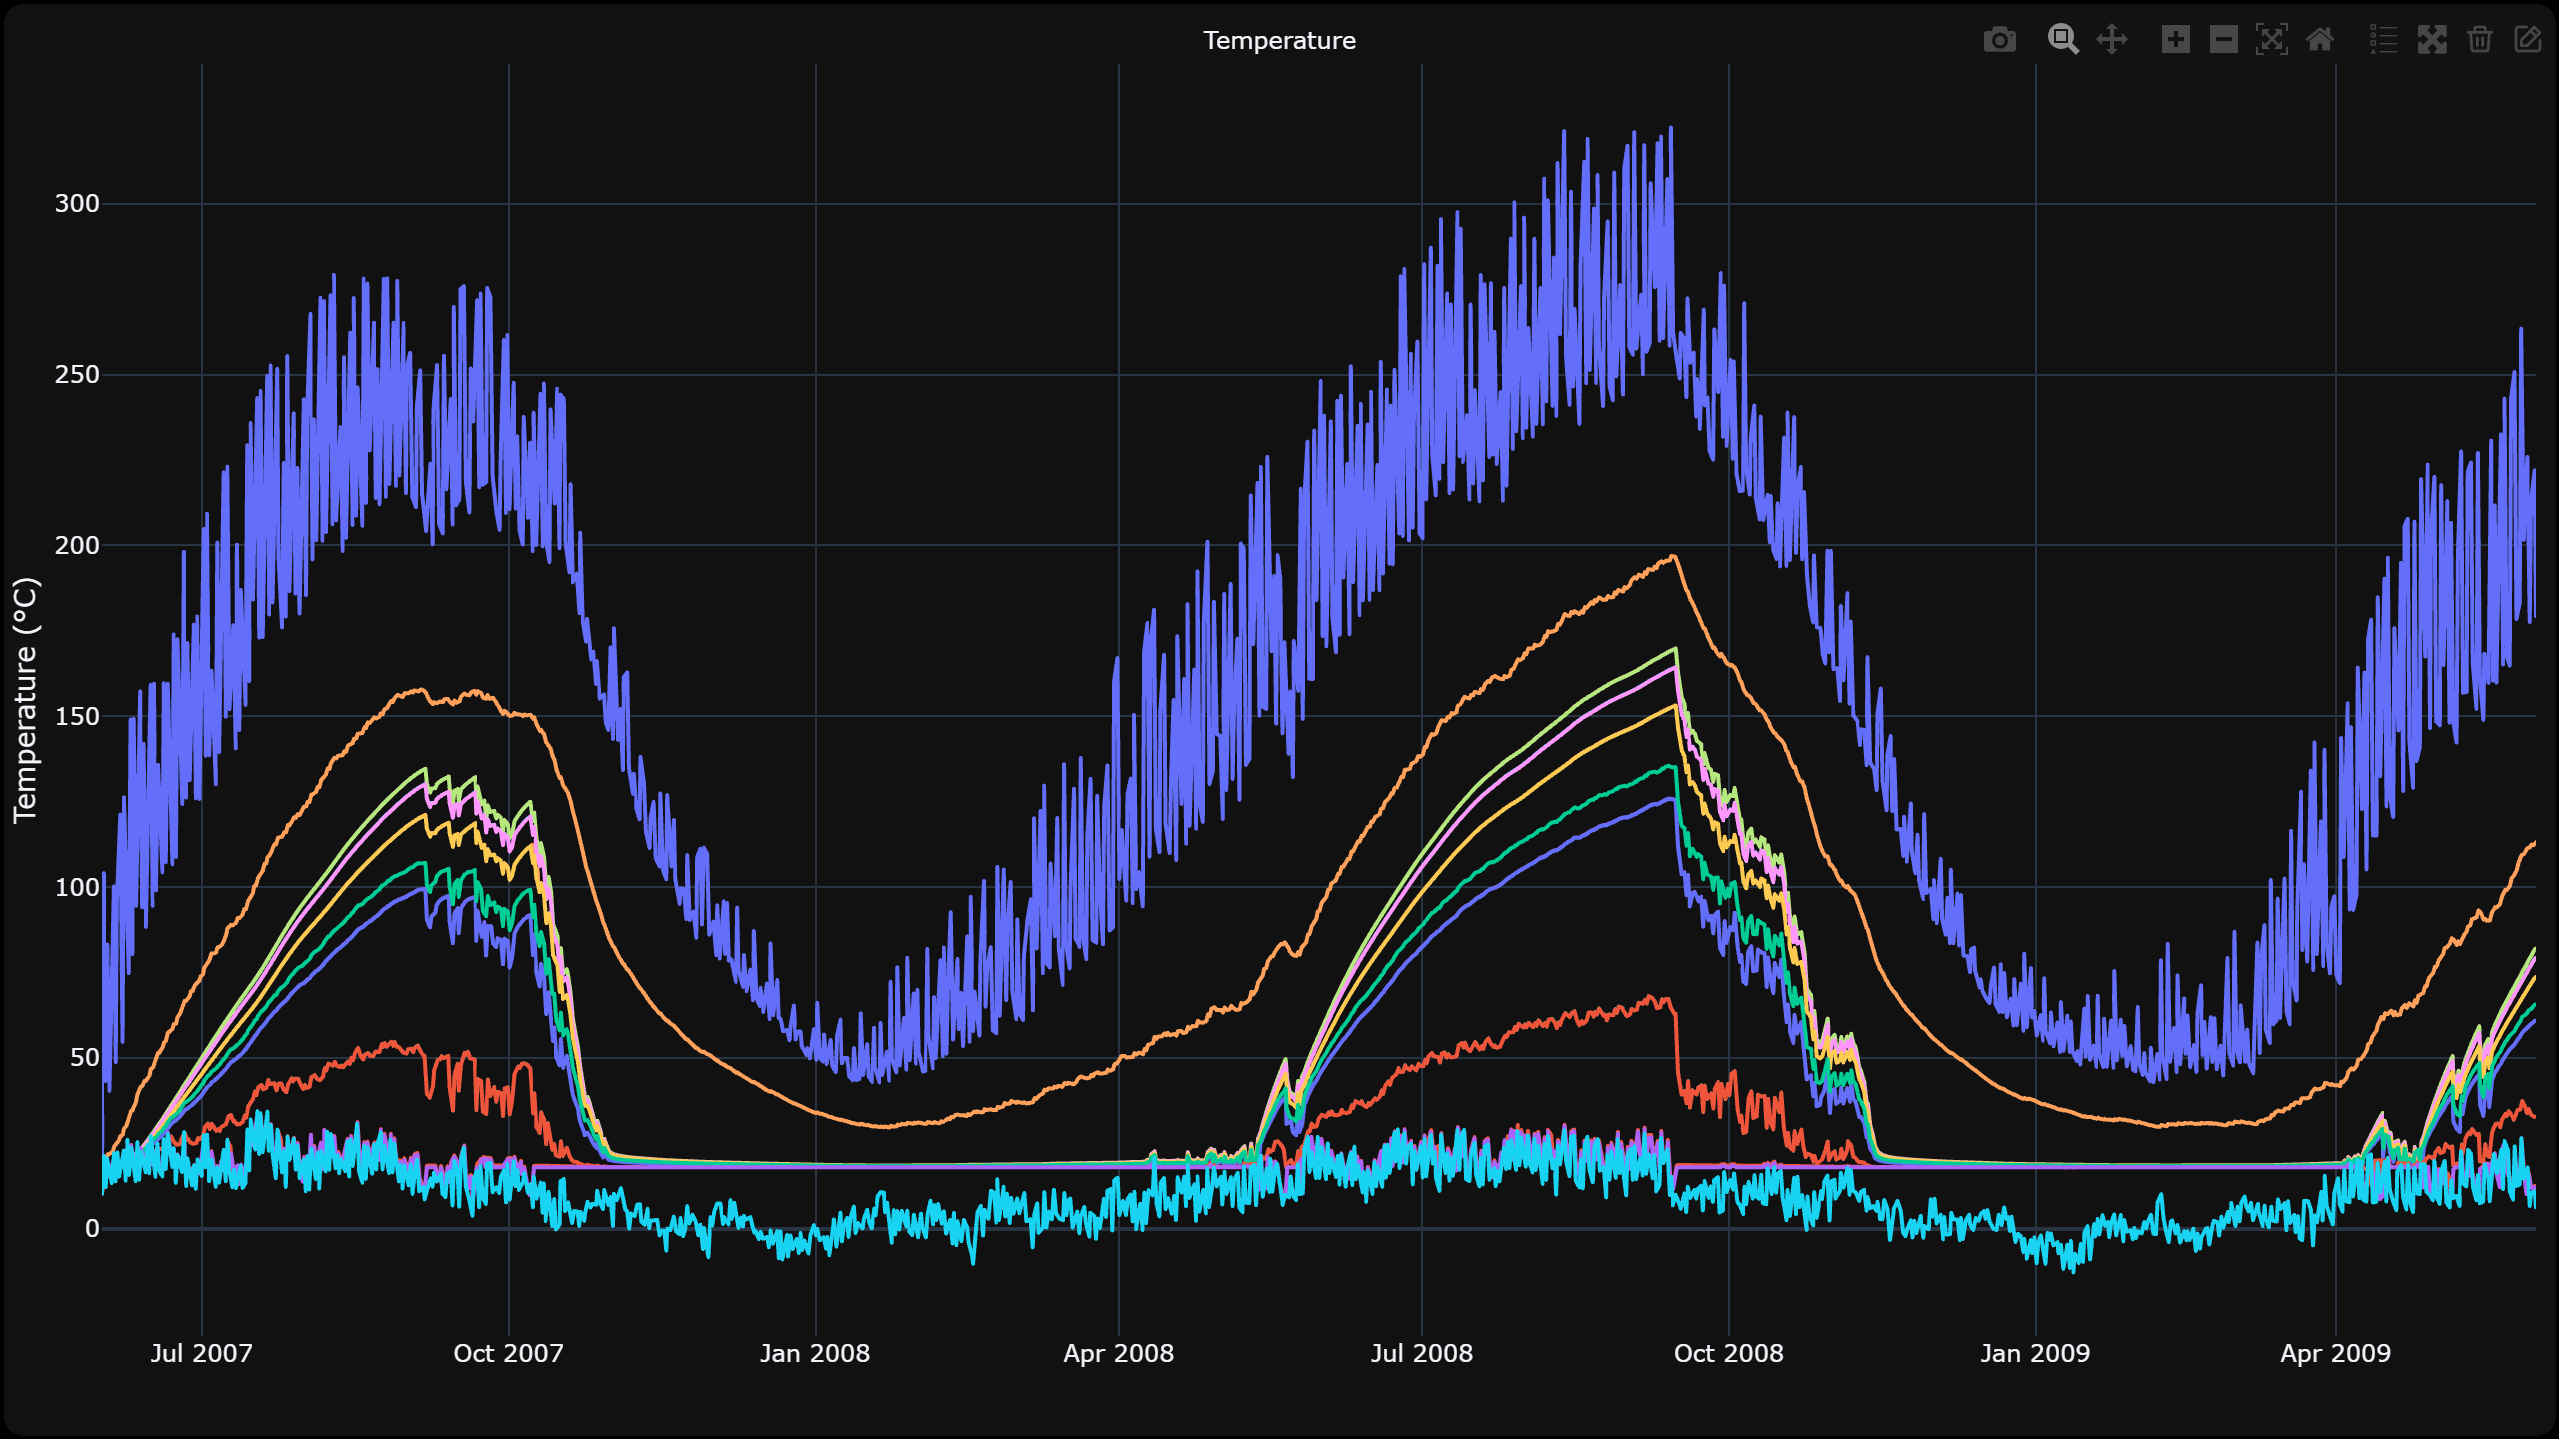
\includegraphics[width=0.98\linewidth]{example_5_result_images/size5-10cartridges.png}
  \caption{Velký akumulátor \(5 \times 5\,\mathrm{m}\) s deseti patronami:
           dvouletý průběh teplot ukazuje sezónní práci zásobníku.}
  \label{fig:c3-size5-10}
\end{figure}

\begin{figure}[H]
  \centering
  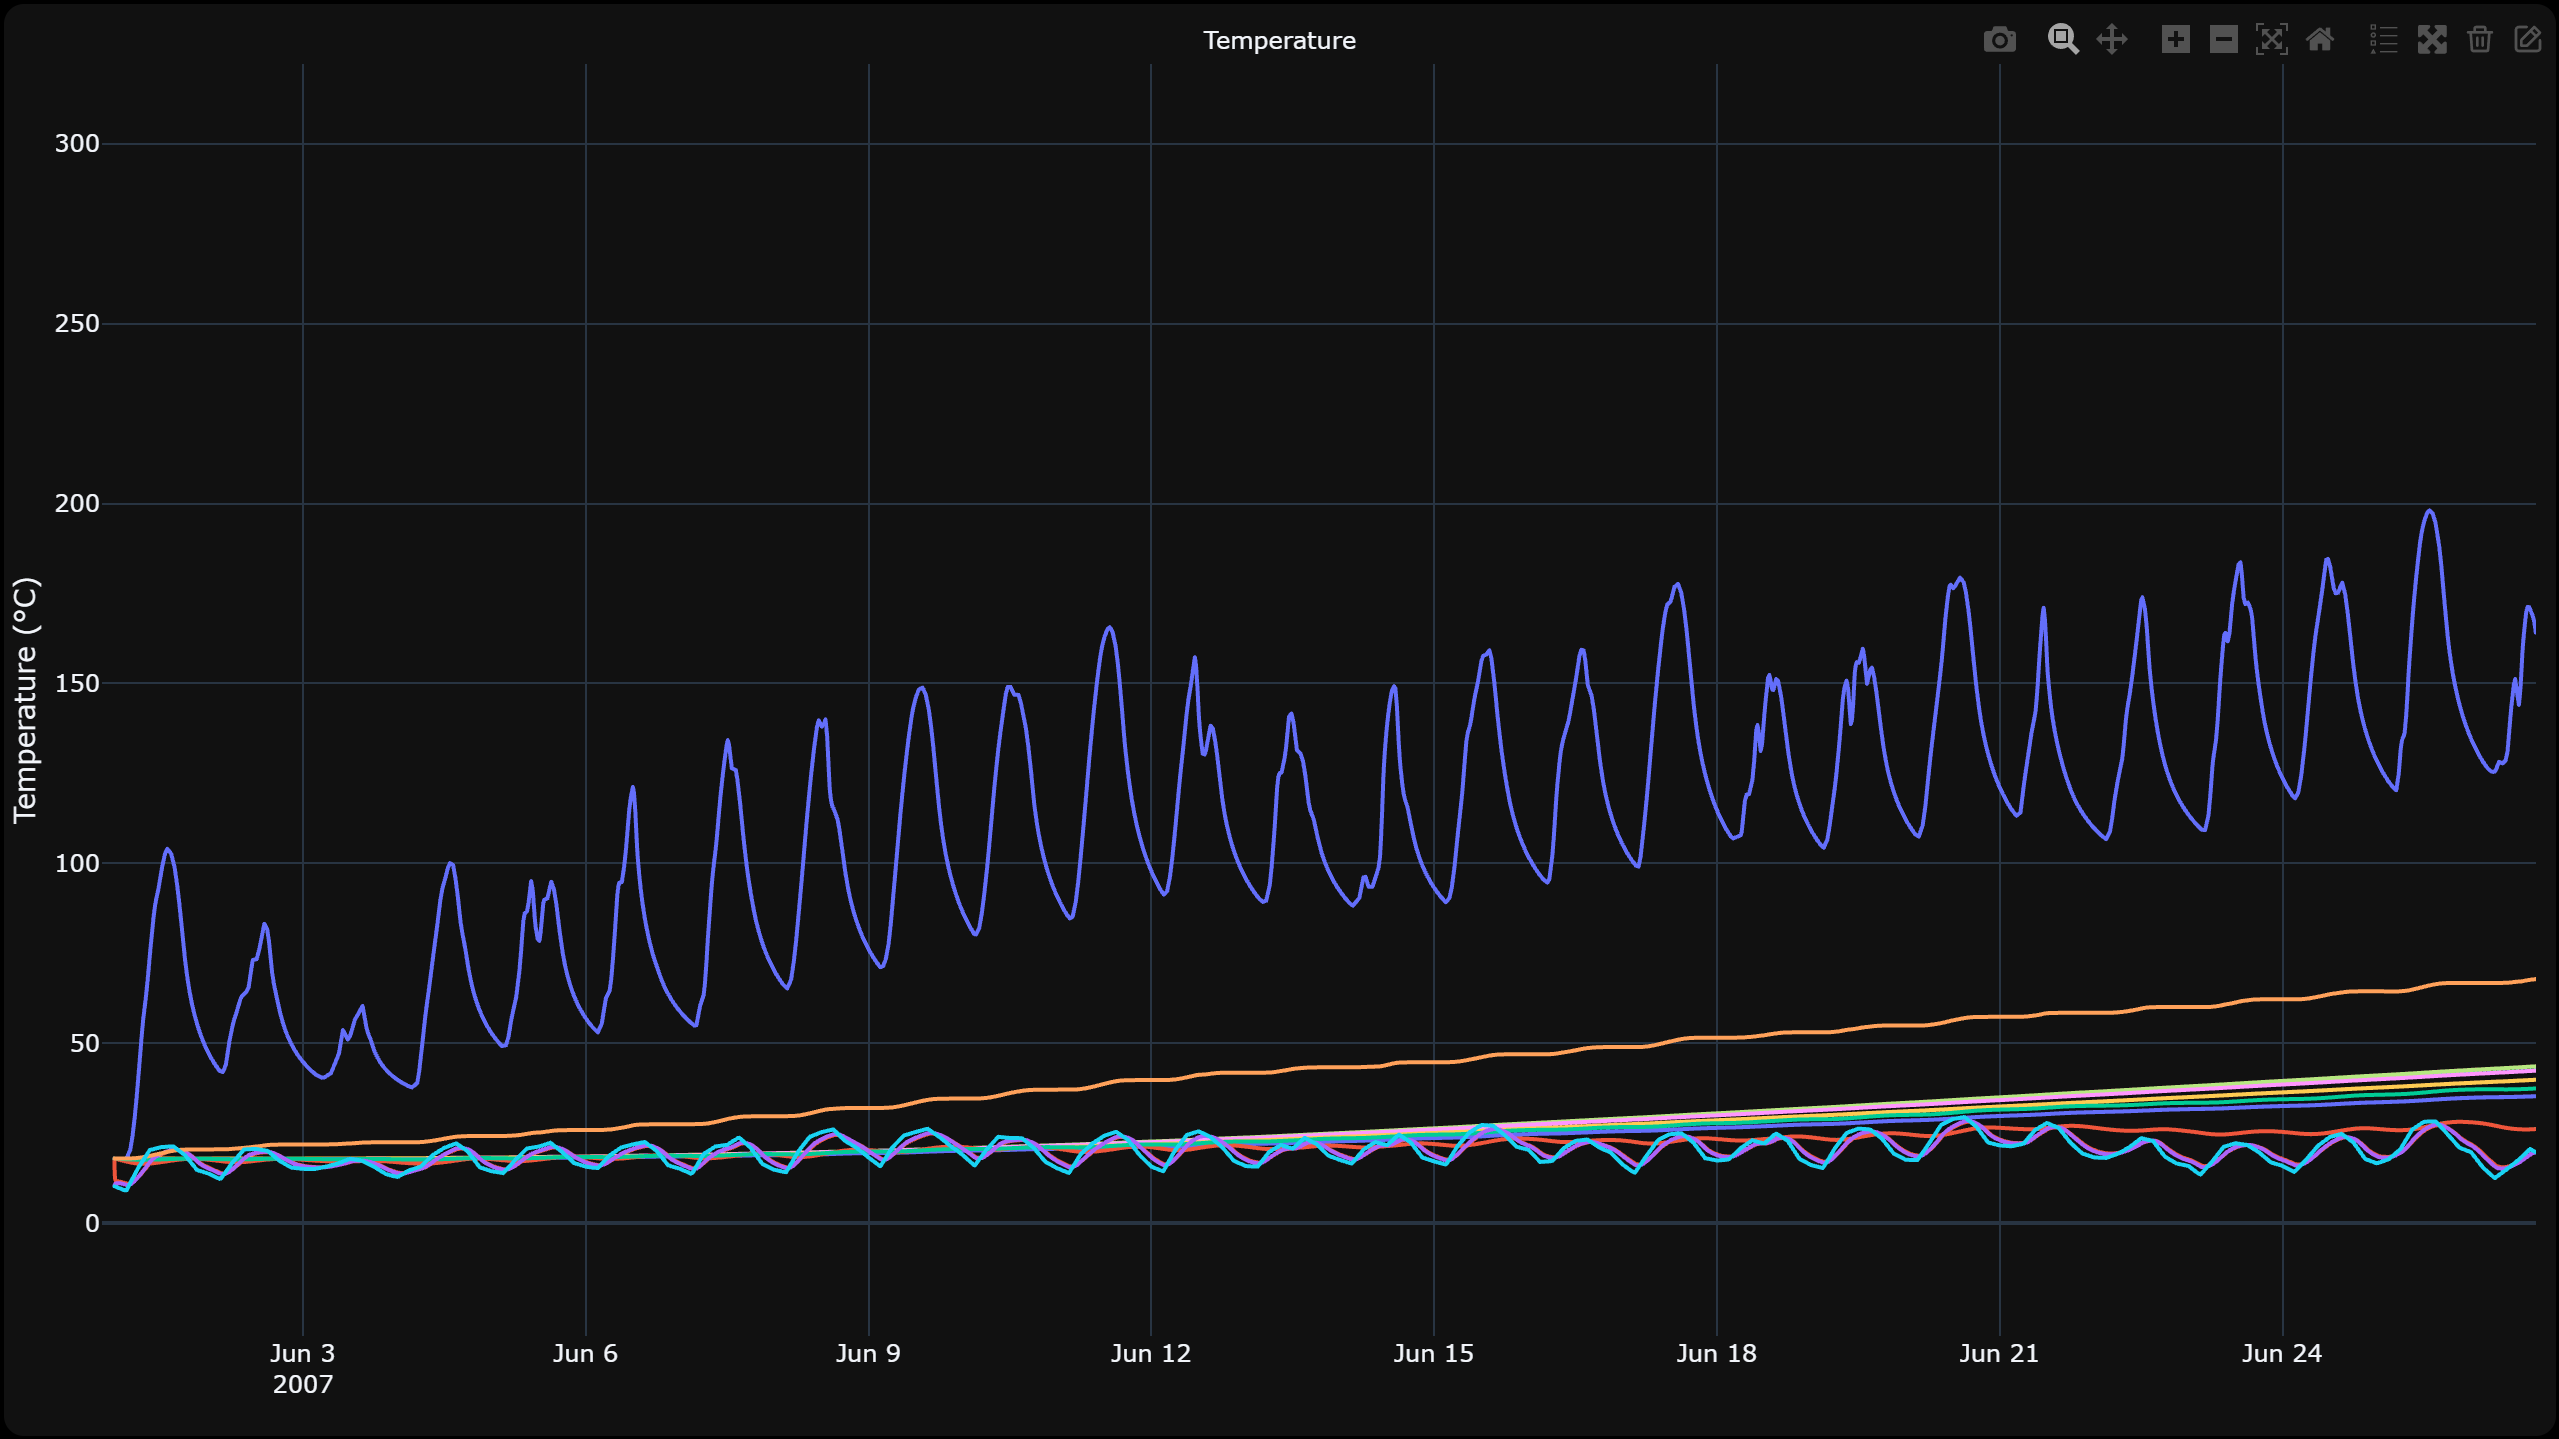
\includegraphics[width=0.98\linewidth]{example_5_result_images/size5-10cartridges-detail.png}
  \caption{Detail velkého akumulátoru \(5 \times 5\,\mathrm{m}\): denní teplotní
           pulzy od FVE a pomalé nabíjení objemu během prvních týdnů.}
  \label{fig:c3-size5-detail}
\end{figure}

\Needspace{9\baselineskip}%
\noindent\begin{minipage}{\linewidth}
\begin{noteblock}
\textbf{Reprodukce obrázků:} screenshoty odpovídají výsledkům z dashboardu
spuštěného nad projektem \texttt{Example\_05}. Jednotlivé konfigurace vznikají
ze slovníku \texttt{ParameterGrid} ve skriptu \path{examples/Example_05/run_example.py}
a ukládají se do PostgreSQL projektu. Dashboard spuštěný přes
\path{examples/Example_05/view_project.py} umožňuje vybrat úlohu v tabulce,
zobrazit časové řady sond a porovnávat varianty podle geometrických parametrů,
počtu patron, uložené energie, tepelných toků a účinností.
\end{noteblock}
\end{minipage}

\subsection*{Co všechno se příklady ověřuje}

Sada příkladů pokrývá hlavní funkcionality balíčku v rozsahu, který je
relevantní pro funkční testování:

\begin{longtable}{@{}L{6.0cm} L{9.0cm}@{}}
\toprule
\textbf{Funkcionalita} & \textbf{Pokryto v} \\
\midrule
\endhead
Procedurální 2D-axisymetrická geometrie (Gmsh)
  & Example\_01 \\
Import geometrie z CAD (\texttt{.step}) + extrakce osové symetrie
  & Example\_02, Example\_03, Example\_04 \\
Plně 3D periodická geometrie (válcová výseč)
  & Example\_05, Example\_06 \\
Term \texttt{UniformHeatSource} + \texttt{AmbientCooling}
  & Example\_01, Example\_02 \\
Nelineární zdroj závislý na teplotě (\(\sigma(T)\))
  & Example\_03 (\texttt{SerialWiresResistiveHeating}) \\
PID regulátor jako Term s implicitní iterací
  & Example\_04 (\texttt{PIDControlledHeatSource}) \\
Ko-simulace se zjednodušeným modelem budovy
  & Example\_05, Example\_06 (\texttt{HallC3}) \\
Stahování meteorologických dat (PVGIS / NSRDB)
  & Example\_05 \\
Parametrická studie (\texttt{ParameterGrid}, KDE řazení)
  & Example\_05 \\
PostgreSQL fronta úloh + MPI workery
  & Example\_05 \\
Webový dashboard s autentizací a RBAC
  & Example\_05 (\texttt{view\_project.py}) \\
Checkpointy a obnova běhu (\texttt{adios4dolfinx})
  & Example\_05, Example\_06 \\
Adaptivní časový krok podle \(\max|\Delta T|\)
  & všechny příklady \\
Sondy do CSV i do databáze
  & Example\_01--04 (CSV), Example\_05 (DB i CSV) \\
\bottomrule
\end{longtable}

Každý příklad lze spustit samostatně a porovnat výstupní CSV
(\texttt{results/unsteady.csv}) s referenčními hodnotami. Regrese se typicky
projeví buď přímo ve fyzikálních sondách (změna zdroje, materiálu nebo okrajové
podmínky), v čítačích \texttt{NLS\_iter\_step} / \texttt{KSP\_iter\_step}
(změna chování řešiče), nebo v agregovaných veličinách \texttt{H\_storage}
a \texttt{Eff\_*} na úrovni celého systému.

% =============================================================================
\section{Časté problémy}\label{sec:faq}

\begin{longtable}{@{}L{5.5cm} L{9.5cm}@{}}
\toprule
\textbf{Projev} & \textbf{Kam se dívat} \\
\midrule
\endhead
SNES / KSP nedoběhne
  & Zmenšete \texttt{dt\_max}, zpřísněte \texttt{dt\_ctrl\_interval}
    a zkontrolujte \texttt{T0} / \texttt{T\_guess}, okrajové podmínky
    i materiály. \\
Worker hlásí prázdnou frontu
  & Zkontrolujte \texttt{-{}-project}, dostupnost databáze a stav úloh
    (\texttt{COMPLETED}, \texttt{RUNNING} apod.). \\
Duplicitně odmítnutá úloha
  & Úloha má stejnou \texttt{SIGNATURE}. Změňte parametry \emph{nebo} zdrojový
    kód tak, aby kombinace dala jiný hash. \\
PVGIS selže
  & Častou příčinou je firewall, timeout nebo špatné souřadnice. Zvyšte
    \texttt{timeout} ve \texttt{fetch\_hourly}; cache lze smazat ručně. \\
Nedostatek místa
  & Zkontrolujte \texttt{checkpoint\_dir}, binární sondy v databázi
    a \texttt{local\_temp\_dir} na výpočetních uzlech. \\
Chyba konfigurace (\texttt{merge\_configs} selhává)
  & Spusťte z adresáře, kde leží správný \texttt{config.yaml}. Nepřidávejte
    klíče mimo \texttt{base\_config.yaml}. \\
Po obnově z checkpointu chybí XDMF časy
  & Pokud při původním běhu \emph{nebyl} XDMF zapnutý, snapshot v checkpointu
    neexistuje a soubor se otevře v režimu \texttt{"w"}. \\
ParaView ukazuje jen mesh, žádné \(T\)
  & Otevřete \texttt{.xdmf}, ne \texttt{.h5}. Případně byl proces ukončen před
    prvním XDMF zápisem (čas \texttt{dt\_xdmf} ještě nenastal). \\
\bottomrule
\end{longtable}

\bigskip
\noindent
\emph{Tento dokument popisuje stav repozitáře v době psaní. Pokud by se návod
a zdrojový kód rozcházely, přednost má \textbf{zdrojový kód}.}

\end{document}
